%% Lecture 7 lecture notes: COMS E6998-019, Designing Production Agentic Systems.
%% Written by slides/tools/notes-doc.py from the speaker notes of lecture7.pptx (slides/slides.primer.json and
%% slides/slides.part2.json); edit the speaker notes in slides/content-primer.py or slides/content-part2.py and run the
%% script again. Build: make (tectonic).

\documentclass[10pt]{extarticle}
\usepackage[margin=2cm]{geometry}
\usepackage[T1]{fontenc}
\usepackage{lmodern,microtype,etoolbox,ragged2e,parskip}
\usepackage{graphicx,caption,booktabs,amsmath,amssymb}
\usepackage[most]{tcolorbox}
\usepackage[colorlinks,linkcolor=violet,citecolor=violet,urlcolor=violet]{hyperref}
\usepackage[noabbrev,nameinlink,capitalise]{cleveref}
\usepackage{tabularx,array,enumitem}
\usepackage[section]{placeins}   % floats never cross into the next section
\makeatletter\g@addto@macro{\UrlBreaks}{\do\-}\makeatother
\captionsetup{font=footnotesize}
\graphicspath{{../slides/figures/}}
\renewcommand\tabularxcolumn[1]{>{\RaggedRight\arraybackslash}p{#1}}
\newcolumntype{L}[1]{>{\RaggedRight\arraybackslash}p{#1}}
\setlength{\tabcolsep}{3pt}
\setlist{nosep, leftmargin=*}
\setlength{\emergencystretch}{3em}
\setlist[enumerate]{label=\arabic*.}
\newcommand{\bi}{\begin{itemize}}
\newcommand{\ei}{\end{itemize}}
\newcommand{\be}{\begin{enumerate}}
\newcommand{\ee}{\end{enumerate}}
\definecolor{deckRose}{HTML}{C73561}
%% the closing box of a slide, in the deck's magenta tint
\newtcolorbox{takeaway}{enhanced, colback=deckRose!8, colframe=deckRose, boxrule=0.5pt, arc=2pt, left=6pt, right=6pt,
  top=3pt, bottom=3pt, fontupper=\bfseries\color{deckRose}, before skip=6pt, after skip=10pt}

\title{Designing Production Agentic Systems\\Lecture 7: OpenShell architecture, and context and compaction}
\author{Rahul Krishna\\Columbia University, COMS E6998-019, Fall 2026}
\date{Draft of November 6, 2026, from the speaker notes of the lecture of November 6, 2026}
\begin{document}
\maketitle
\begin{abstract}
These notes collect the speaker notes of Lecture 7, one part for each half of the lecture: OpenShell architecture, then Context and compaction. Each part opens with the note of its route slide.
\end{abstract}
\tableofcontents

\part{OpenShell architecture}
Introduce the OpenShell refresher. Lecture 6 worked with OpenShell 0.1.4, and some students missed it. This part follows NVIDIA's architecture page for the current release, documentation version v0.1.7, in its five sections: what each piece does, the sandbox boundary, the path of a network request, how each runtime builds the boundary, and how the components authenticate. The slides condense the page's text and reveal its four figures one part per click. The notes keep the page's own wording. Source: NVIDIA, OpenShell Developer Guide, ``Architecture'', documentation version v0.1.7, read on November 6, 2026 (\url{https://docs.nvidia.com/openshell/v0.1.7/about/architecture}).

\section{What each piece does}
\label{sec:row-p1-0}

We start with the two ways OpenShell governs an agent, then the pieces that do it and the job of each.

\subsection{OpenShell enforces and verifies policy}
\label{sec:it-os-1-1}

\bi
\item \textbf{Kernel-level enforcement:} kernel controls confine each agent's files and system calls, and every connection passes a policy check.
\item \textbf{Verified policy changes:} formal verification flags risky new access that a change would grant, and that change waits for human review.
\ei

The page opens with the two ways OpenShell governs what agents can do. It instruments the kernel to enforce policy on every file access, system call and network connection at runtime, and it uses formal verification to check what a policy change would allow before it is applied.

Kernel-level enforcement: each agent runs in an isolated sandbox. Kernel controls confine which files it can access and which system calls it can make, and every network connection passes through a policy check before it leaves the sandbox. Agents never see real credentials. OpenShell adds them only to requests bound for approved endpoints.

Formally verified policy changes: before a policy change is approved, OpenShell uses formal verification to flag risky new access it would grant, such as reaching a new host with credentials or calling a new API method, so those changes wait for human review.

The figure is the policy lifecycle strip from the bottom of NVIDIA's system architecture figure. In the full figure, both dashed lines run up to the supervisor, so a copy of the supervisor's box sits above the strip here. The next slide shows the rest of the figure: the gateway, and the supervisor's duties.

The figure is NVIDIA's own, from the same page, under the Apache-2.0 license. Its text is unchanged, and the slide reveals it one part per click. Source: NVIDIA, OpenShell Developer Guide, ``Architecture'', documentation version v0.1.7, read on November 6, 2026 (\url{https://docs.nvidia.com/openshell/v0.1.7/about/architecture}).

\begin{figure}[htbp]
\centering
\includegraphics[width=\linewidth]{openshell/os-policy-lifecycle-4.png}
\caption{OpenShell enforces and verifies policy. The figure as it stands after the build's last click.}
\label{fig:os-policy-lifecycle-4}
\end{figure}

\paragraph{The figure, stage by stage.}
\be
\item The agent proposes a policy change ``via policy.local'', and the supervisor sends it on (``supervisor proposes'').
\item The gateway's policy prover checks the change and ``flags risky new access''.
\item A person approves it: ``manual by default'', or automatically when the prover finds no new risk.
\item The approved policy reloads into the supervisor, which ``retries'' (``approved policy reloaded'').
\ee

\begin{takeaway}OpenShell enforces policy while the agent runs and checks each policy change before it applies.\end{takeaway}

\subsection{The gateway manages every sandbox}
\label{sec:it-os-1-2}

The gateway is the control plane. It manages the lifecycle of sandboxes and provides connectivity and management of sandboxes to end users and operators. When a user creates a sandbox, its compute driver provisions a workload and a separate supervisor, establishes their protected channel, and builds the isolation boundary. The supervisor confirms that boundary before starting the agent, and then connects back to the gateway for policy, credentials, logs and interactive sessions.

This is NVIDIA's system architecture figure without its policy lifecycle strip, which the previous slide showed. The two dashed lines that join the supervisor to that strip are left out here.

The figure is NVIDIA's own, from the same page, under the Apache-2.0 license. Its text is unchanged, and the slide reveals it one part per click. Source: NVIDIA, OpenShell Developer Guide, ``Architecture'', documentation version v0.1.7, read on November 6, 2026 (\url{https://docs.nvidia.com/openshell/v0.1.7/about/architecture}).

\begin{figure}[htbp]
\centering
\includegraphics[width=\linewidth]{openshell/os-architecture-3.png}
\caption{The gateway manages every sandbox. The figure as it stands after the build's last click.}
\label{fig:os-architecture-3}
\end{figure}

\paragraph{The figure, stage by stage.}
\be
\item The control plane. The CLI, the SDK and the TUI reach the gateway over gRPC or HTTP. Inside the gateway sit the API server (``API, authentication, lifecycle, relays''), the policy prover, the durable state (``sandboxes, policies, providers, settings'') and the compute driver, which ``places and fences each sandbox''.
\item The data plane. The compute driver starts the runtime. The supervisor ``governs the agent'': policy evaluation, credential resolution, DNS and proxying, agent session multiplexing, and it maintains the gateway session. Beside it, the network-isolated sandbox (a container or a VM) holds the sandbox, the ``process owner and syscall boundary'', and the agent, the ``untrusted workload''.
\item The network. The mediated channel from the sandbox to the supervisor is the workload's only way out: the workload network rule says ``deny all egress, except to the supervisor'', and only the supervisor's ``policy-approved egress'' reaches external services and models.
\ee

\begin{takeaway}The gateway manages every sandbox, and the supervisor confirms its boundary before the agent starts.\end{takeaway}

\subsection{Each piece of OpenShell has its own job}
\label{sec:it-os-1-3}

\textbf{The supervisor row holds every policy decision.}

This is the page's table ``What Each Piece Does'', one row per click, in the page's order from the sandbox outward. The cells are shortened. The page's full entries follow.

Sandbox: lives inside the boundary with the agent. It owns the agent's processes, knows which program made each request, applies process controls, and forwards TCP and DNS traffic to the supervisor.

Outer network fence: denies all network egress from the workload except its protected connection to the supervisor. Each runtime builds this with its own native tools.

Supervisor: lives on the trusted side of the boundary. It checks requests against policy, supplies credentials, resolves DNS, opens approved connections, and keeps the link to the gateway alive. It works with every runtime through one isolation backend interface to confirm the boundary, start the agent, run commands, forward connections, and see network requests.

Policies: describe what the agent can touch: files, processes, network destinations, API calls, and where provider credentials can go.

Providers: connect a service name to a stored credential. The supervisor hands that credential out only where policy allows it.

Policy prover: runs in the gateway and uses formal verification to check agent-proposed network rules. It flags changes such as new credentialed reach, new HTTP methods, or access to cloud metadata endpoints, and any finding blocks auto-approval. It also ships as the standalone openshell-prover command for checking a policy against a boundary in CI.

Gateway: checks who the user is and remembers everything about the sandboxes. It delivers policy and settings, attaches providers, decides who can do what, and coordinates connections into sandboxes.

Compute runtime: creates the sandbox, starts the supervisor and the workload, sets up the private channel between them, and builds the network fence. It reports status back and cleans up when the sandbox goes away.

Source: NVIDIA, OpenShell Developer Guide, ``Architecture'', documentation version v0.1.7, read on November 6, 2026 (\url{https://docs.nvidia.com/openshell/v0.1.7/about/architecture}).

\begin{center}\footnotesize
\begin{tabularx}{\linewidth}{L{0.22\linewidth}X}
\toprule
\textbf{Piece} & \textbf{What it does} \\
\midrule
Sandbox & Owns the agent's processes and forwards TCP and DNS traffic to the supervisor. \\
Outer network fence & Denies all workload egress except the protected connection to the supervisor. \\
Supervisor & Checks requests against policy, supplies credentials and opens approved connections. \\
Policies & Describe what the agent can touch, from files to where credentials can go. \\
Providers & Connect a service name to a stored credential. \\
Policy prover & Uses formal verification to check agent-proposed network rules. \\
Gateway & Checks who each user is, keeps every sandbox's record and delivers policy. \\
Compute runtime & Creates the sandbox, starts the supervisor and the workload, and builds the fence. \\
\bottomrule
\end{tabularx}
\end{center}

\begin{takeaway}The gateway manages, the supervisor decides, and the sandbox reports from beside the agent.\end{takeaway}

\subsection*{Key points}
\bi
\item OpenShell enforces policy while the agent runs and checks each policy change before it applies.
\item The gateway manages every sandbox, and the supervisor confirms its boundary before the agent starts.
\item The gateway manages, the supervisor decides, and the sandbox reports from beside the agent.
\ei

\section{Inside the sandbox boundary}
\label{sec:row-p1-1}

Next, the boundary itself: which side decides, and what the side next to the agent provides.

\subsection{Only the supervisor makes policy decisions}
\label{sec:it-os-2-1}

\bi
\item \textbf{The sandbox} shares the boundary with the untrusted agent, so it reports what the agent tries to do.
\item \textbf{The supervisor} sits on the trusted side and makes every policy decision.
\item \textbf{In the Linux backend,} the workload runs as one non-root identity with no Linux capabilities, under Landlock and seccomp.
\ei

The supervisor and the sandbox sit on opposite sides of the boundary. The supervisor is trusted and makes the decisions. The sandbox shares the boundary with the untrusted agent, so it never makes policy decisions. It reports what the agent is trying to do and lets the supervisor decide.

The sandbox launches the agent as an owned child and provides exec, terminal streams, signals, process status and loopback forwarding. In the current Linux backend, the workload uses one non-root identity and no Linux capabilities. Landlock limits filesystem access, and seccomp user notification stages network operations. The sandbox identifies the calling executable from trusted process observations.

The figure is NVIDIA's own, from the same page, under the Apache-2.0 license. Its text is unchanged, and the slide reveals it one part per click. Source: NVIDIA, OpenShell Developer Guide, ``Architecture'', documentation version v0.1.7, read on November 6, 2026 (\url{https://docs.nvidia.com/openshell/v0.1.7/about/architecture}).

\begin{figure}[htbp]
\centering
\includegraphics[width=\linewidth]{openshell/os-enforcement-4.png}
\caption{Only the supervisor makes policy decisions. The figure as it stands after the build's last click.}
\label{fig:os-enforcement-4}
\end{figure}

\paragraph{The figure, stage by stage.}
\be
\item The sandbox side. The agent, a process, sends a TCP or DNS request to the OpenShell Sandbox (arrow 1), which owns the process and identifies the program. All other egress from the container or VM is denied.
\item The request crosses the Sandbox Protocol, the ``only allowed egress'', over a Unix socket, TCP or vsock (arrow 2), to the supervisor's isolation backend, which verifies the boundary and ``receives request with trusted process identity''.
\item Policy enforcement ``checks destination, binary, L7 rules, and credentials'' (arrow 3), and an approved connection reaches the upstream service (arrow 4).
\item policy.local carries proposed policy changes from the sandbox to the supervisor, and approved ones reload, asynchronously.
\ee

\begin{takeaway}Policy decisions stay on the trusted side of the boundary, out of the agent's reach.\end{takeaway}

\subsection{One authenticated link carries all streams}
\label{sec:it-os-2-2}

\bi
\item \textbf{The Sandbox Protocol} is one mutually authenticated HTTP/2 connection.
\item \textbf{Each TCP connection} gets its own stream with its own backpressure.
\ei

The supervisor and the sandbox talk over the OpenShell Sandbox Protocol: one mutually authenticated HTTP/2 connection that carries many independent streams. The compute driver picks the transport: a Unix socket for Docker and Podman, TCP for Kubernetes, or vsock for MicroVM. Authentication and protocol behavior are the same on all of them. The supervisor presents a sandbox-specific credential, which the section on authentication describes.

Each TCP connection gets its own stream with its own backpressure, so a slow download can't block DNS, exec, or process control.

The figure is NVIDIA's own, from the same page, under the Apache-2.0 license. Its text is unchanged, and the slide reveals it one part per click. Source: NVIDIA, OpenShell Developer Guide, ``Architecture'', documentation version v0.1.7, read on November 6, 2026 (\url{https://docs.nvidia.com/openshell/v0.1.7/about/architecture}).

\begin{figure}[htbp]
\centering
\includegraphics[width=\linewidth]{openshell/os-protocol-3.png}
\caption{One authenticated link carries all streams. The figure as it stands after the build's last click.}
\label{fig:os-protocol-3}
\end{figure}

\paragraph{The figure, stage by stage.}
\be
\item The two ends. The trusted supervisor does policy evaluation, credential injection, DNS resolution and upstream connections, and holds the gateway session. The network-isolated sandbox owns the agent process, identifies each program, intercepts TCP and DNS, and freezes the agent on disconnect.
\item One mutually authenticated HTTP/2 connection joins them. Its control stream carries ``attach, confirm, start, exec, signals, health''. The transport is a Unix socket for Docker and Podman, TCP for Kubernetes, or vsock for MicroVM, and authentication and protocol behavior stay the same.
\item DNS gets its own stream (``query and mediated response''), and so does each TCP connection (``destination, program identity, bytes''), each with ``independent connection and backpressure''.
\ee

\begin{takeaway}A slow download on one stream can't block DNS, exec or process control on the others.\end{takeaway}

\subsection{What the sandbox guarantees the supervisor}
\label{sec:it-os-2-3}

\textbf{Each row pairs what the sandbox does with what the supervisor gets.}

This is the page's table of guarantees, one row per click. The program identity row reads ``The real program behind each request, not a path the agent claims'' on the page. The slide says it without the contrast.

Together these mean the agent can't run before its controls are confirmed, signals and exec reach only this sandbox's processes, and the agent can't get around TCP or DNS mediation.

Source: NVIDIA, OpenShell Developer Guide, ``Architecture'', documentation version v0.1.7, read on November 6, 2026 (\url{https://docs.nvidia.com/openshell/v0.1.7/about/architecture}).

\begin{center}\footnotesize
\begin{tabularx}{\linewidth}{L{0.22\linewidth}XX}
\toprule
\textbf{Guarantee} & \textbf{How the sandbox provides it} & \textbf{What the supervisor gets} \\
\midrule
Process ownership & Runs the agent as an owned child and keeps its process and terminal state. & Handles to wait on, attach to, signal, exec in, and stop the agent. \\
Program identity & Identifies the calling program from trusted /proc data. & The real program behind each request, whatever path the agent claims. \\
Network mediation & Intercepts TCP opens and DNS queries with seccomp and hands them over. & Requests that wait for a policy decision before going anywhere. \\
Fail closed & Holds launch until the supervisor confirms, and freezes the agent if the connection drops. & A short window to reconnect, or a stopped workload. \\
\bottomrule
\end{tabularx}
\end{center}

\begin{takeaway}The agent can't run before its controls are confirmed or get around TCP and DNS mediation.\end{takeaway}

\subsection*{Key points}
\bi
\item Policy decisions stay on the trusted side of the boundary, out of the agent's reach.
\item A slow download on one stream can't block DNS, exec or process control on the others.
\item The agent can't run before its controls are confirmed or get around TCP and DNS mediation.
\ei

\section{How a network request travels}
\label{sec:row-p1-2}

Now one request, from the agent's connect call to the upstream service.

\subsection{Every request leaves through the supervisor}
\label{sec:it-os-3-1}

\bi
\item \textbf{1.} The agent opens a TCP connection or makes a DNS lookup.
\item \textbf{2.} The sandbox identifies the calling program.
\item \textbf{3.} The request travels over the Sandbox Protocol to the supervisor.
\item \textbf{4.} The supervisor checks it against policy and adds allowed credentials.
\item \textbf{5.} If allowed, the supervisor opens the real connection and relays traffic.
\ei

These are the page's five steps of a network request, one per click.

The mediated channel to the supervisor is the workload's only allowed egress path. The outer fence denies everything else, so the agent can't reach a service, the gateway, DNS, or another private address directly.

The figure is NVIDIA's own, from the same page, under the Apache-2.0 license. Its text is unchanged, and the slide reveals it one part per click. Source: NVIDIA, OpenShell Developer Guide, ``Architecture'', documentation version v0.1.7, read on November 6, 2026 (\url{https://docs.nvidia.com/openshell/v0.1.7/about/architecture}).

The figure is \cref{fig:os-enforcement-4} of \cref{sec:it-os-2-1}.

\paragraph{The figure, stage by stage.}
\be
\item The enforcement figure of the section ``Inside the sandbox boundary'', complete. Its arrows follow the request: arrow 1 is steps 1 and 2 (the agent's request, and the sandbox identifying the program), arrow 2 is step 3 (the Sandbox Protocol), arrow 3 is step 4 (policy enforcement adds credentials), and arrow 4 is step 5 (the real connection to the upstream service).
\ee

\begin{takeaway}The outer fence denies every other path, so the agent can't reach any address directly.\end{takeaway}

\subsection{The supervisor relays the agent's traces itself}
\label{sec:it-os-3-2}

\bi
\item \textbf{The trace relay:} when an operator enables it, the sandbox points the agent's OpenTelemetry SDK at the reserved address \texttt{192.0.0.8:4318}.
\item \textbf{The supervisor} answers those connections itself, tags each trace batch with the sandbox ID and forwards it to the operator's collector.
\item \textbf{The agent} never learns the collector's address and needs no egress rule to reach it.
\ei

When an operator enables the agent trace relay, the sandbox points the agent's OpenTelemetry SDK at the reserved address 192.0.0.8:4318. Connections to it take the same mediated channel, but the supervisor answers them itself instead of opening an upstream connection. It tags each trace batch with the sandbox ID and forwards it to the operator's collector. The agent never learns the collector's address and needs no egress rule to reach it.

Source: NVIDIA, OpenShell Developer Guide, ``Architecture'', documentation version v0.1.7, read on November 6, 2026 (\url{https://docs.nvidia.com/openshell/v0.1.7/about/architecture}).

\begin{takeaway}Traces travel the mediated channel and open no new path out of the sandbox.\end{takeaway}

\subsection*{Key points}
\bi
\item The outer fence denies every other path, so the agent can't reach any address directly.
\item Traces travel the mediated channel and open no new path out of the sandbox.
\ei

\section{How each runtime builds the boundary}
\label{sec:row-p1-3}

The boundary is the same contract on every runtime, built with different tools.

\subsection{Each runtime builds the boundary its own way}
\label{sec:it-os-4-1}

\textbf{Every runtime follows the same contract.}

Every runtime follows the same contract, but each one uses the tools it already has to place the supervisor, connect it to the sandbox, and fence off the network. The table is the page's, one row per click.

The runtime's job is to build the boundary and prove it's in place. It never decides whether a request is allowed. That decision always belongs to the shared supervisor and policy engine, which is why the same policy behaves the same way everywhere. Runtimes can differ in how they report readiness and which features they support. Each one advertises its capabilities so the gateway knows what it can do.

The page ends with existing infrastructure. OpenShell plugs into the tools a team already uses, including container runtimes, schedulers, secret stores, identity providers, image pipelines, storage and device plugins. The gateway and the supervisor define how OpenShell behaves. Drivers translate that behavior into whatever the platform understands and report back what happened, which keeps platform-specific details out of the core control plane and the policy model.

Source: NVIDIA, OpenShell Developer Guide, ``Architecture'', documentation version v0.1.7, read on November 6, 2026 (\url{https://docs.nvidia.com/openshell/v0.1.7/about/architecture}).

\begin{center}\footnotesize
\begin{tabularx}{\linewidth}{L{0.22\linewidth}XXX}
\toprule
\textbf{Runtime} & \textbf{Where the supervisor runs} & \textbf{How it talks to the sandbox} & \textbf{How direct egress is blocked} \\
\midrule
Docker & Its own container & Authenticated Unix socket on a driver-owned volume & Workload container has networking turned off \\
Podman & Its own container & Authenticated Unix socket on a driver-owned volume & Workload container has networking turned off \\
Kubernetes & Its own pod & Private service with mutual TLS & NetworkPolicy allows only the supervisor service \\
VM & A process on the host & Authenticated vsock & Guest has no network device \\
\bottomrule
\end{tabularx}
\end{center}

\begin{takeaway}The runtime builds and proves the boundary, and the shared supervisor decides every request.\end{takeaway}

\subsection*{Key points}
\bi
\item The runtime builds and proves the boundary, and the shared supervisor decides every request.
\ei

\section{How components authenticate}
\label{sec:row-p1-4}

Last, the credentials that tie a sandbox together, and what the agent can see of them.

\subsection{The gateway signs every credential}
\label{sec:it-os-5-1}

\bi
\item \textbf{The gateway} is the only component that signs credentials, and every credential names exactly one sandbox.
\item \textbf{The first credential} comes from the compute driver, in files only the supervisor can read, or on Kubernetes as the pod's ServiceAccount token.
\ei

Three connections tie a sandbox together. The gateway is the only component that signs credentials, and every credential names exactly one sandbox.

The supervisor needs a starting credential to prove which sandbox it belongs to, and how it gets one depends on the runtime. With Docker, Podman and MicroVM, the driver hands the supervisor its initial tokens directly, in files only the supervisor can read. On Kubernetes, the supervisor presents its pod's ServiceAccount token, and the gateway asks the Kubernetes driver to verify the token and confirm that the pod belongs to the expected sandbox before it issues any JWTs. Either way, the gateway checks the claim against its own record of the sandbox before returning credentials.

The figure is NVIDIA's own, from the same page, under the Apache-2.0 license. Its text is unchanged, and the slide reveals it one part per click. Source: NVIDIA, OpenShell Developer Guide, ``Architecture'', documentation version v0.1.7, read on November 6, 2026 (\url{https://docs.nvidia.com/openshell/v0.1.7/about/architecture}).

\begin{figure}[htbp]
\centering
\includegraphics[width=\linewidth]{openshell/os-authentication-4.png}
\caption{The gateway signs every credential. The figure as it stands after the build's last click.}
\label{fig:os-authentication-4}
\end{figure}

\paragraph{The figure, stage by stage.}
\be
\item The parties. The gateway's API server ``signs every JWT'' and ``checks the sandbox record''. Its compute driver ``delivers or verifies the bootstrap credential''. The supervisor ``holds tokens in memory''. The sandbox ``verifies, never signs'', and the agent ``sees no credentials''.
\item 1, bootstrap: the compute driver gives the supervisor its starting credential.
\item 2 and 3: the supervisor authenticates to the API server, which issues the JWT pair, a gateway JWT for the gateway and a sandbox JWT for the sandbox.
\item 4: the supervisor presents the sandbox JWT to the sandbox over mutual TLS. The line under the figure: every JWT names one sandbox and one run of it, and restarting a sandbox issues new tokens and TLS certificates.
\ee

\begin{takeaway}A credential works for exactly one sandbox, and only the gateway can sign one.\end{takeaway}

\subsection{Each connection has its own protection}
\label{sec:it-os-5-2}

\textbf{The agent never connects to the supervisor itself.}

This is the page's table of connections, one row per click. In the last row the page says the sandbox relays the agent's traffic over the connection above, the supervisor-to-sandbox channel.

The supervisor verifies the gateway's TLS certificate with its CA. User client certificates and private keys stay outside both the supervisor and the workload, and the gateway JWT authenticates supervisor RPCs.

Source: NVIDIA, OpenShell Developer Guide, ``Architecture'', documentation version v0.1.7, read on November 6, 2026 (\url{https://docs.nvidia.com/openshell/v0.1.7/about/architecture}).

\begin{center}\footnotesize
\begin{tabularx}{\linewidth}{L{0.22\linewidth}XX}
\toprule
\textbf{Connection} & \textbf{Who connects} & \textbf{How it's protected} \\
\midrule
Supervisor to gateway & The supervisor dials out to the gateway. & A gateway JWT, over TLS when the gateway has TLS enabled. \\
Supervisor to sandbox & The supervisor dials into the workload over the driver's private channel. & Mutual TLS, plus a sandbox JWT. \\
Agent to supervisor & The agent never connects directly. The sandbox relays its traffic. & Covered by the supervisor-to-sandbox channel. \\
\bottomrule
\end{tabularx}
\end{center}

\begin{takeaway}The sandbox relays the agent's traffic over the supervisor's authenticated channel.\end{takeaway}

\subsection{Each token is bound to one sandbox run}
\label{sec:it-os-5-3}

\bi
\item \textbf{The gateway JWT} goes with every supervisor call to the gateway and allows only the calls a supervisor needs.
\item \textbf{The sandbox JWT} goes with every supervisor call to the sandbox, which holds only the gateway's public key, so it can verify the token and never create one.
\item \textbf{A restart} starts a new generation with fresh tokens and TLS certificates, and the old ones stop working.
\item \textbf{Renewal} happens in memory and only while the sandbox exists, so deleting a sandbox cuts off its supervisor.
\ei

The gateway issues a pair of JWTs for each run of a sandbox. The gateway JWT is sent with every supervisor call to the gateway. It allows only the calls a supervisor needs, such as fetching policy, pushing logs and relaying sessions. It is not a user credential and can't manage other sandboxes. The sandbox JWT is sent with every supervisor call to the sandbox. The sandbox holds only the gateway's public key, so it can verify the token but can never create one.

Each token works only on its own connection. Both are bound to one sandbox and one run of that sandbox, called a generation. Restarting a sandbox starts a new generation with fresh tokens and fresh TLS certificates, and the old ones stop working.

Renewing and revoking: the supervisor keeps its tokens in memory and renews both together before they expire. Renewal works only while the sandbox still exists, so deleting a sandbox cuts off its supervisor. Shared deployments, such as Kubernetes, should set gateway\_jwt.ttl\_secs so tokens expire. Local single-user gateways can leave it unset, which issues tokens that last for the life of the sandbox run.

Source: NVIDIA, OpenShell Developer Guide, ``Architecture'', documentation version v0.1.7, read on November 6, 2026 (\url{https://docs.nvidia.com/openshell/v0.1.7/about/architecture}).

\begin{takeaway}A token is bound to one connection, one sandbox and one generation.\end{takeaway}

\subsection{The sandbox holds nothing worth stealing}
\label{sec:it-os-5-4}

\bi
\item \textbf{No secrets:} the sandbox holds no gateway signing key, no gateway JWT and no provider credentials.
\item \textbf{No impersonation:} the sandbox can verify that it talks to the right supervisor and can't pose as one.
\item \textbf{A disconnect} freezes the agent, and only the same supervisor process can reconnect and resume it.
\ei

The agent shares its side of the boundary with the sandbox, so the sandbox holds nothing worth stealing: no gateway signing key, no gateway JWT, and no provider credentials. It can verify that it's talking to the right supervisor, but it can't impersonate one.

If the supervisor disconnects, the sandbox freezes the agent. Only the same supervisor process can reconnect and resume it. A new supervisor can't take over a running sandbox, even with valid credentials.

Source: NVIDIA, OpenShell Developer Guide, ``Architecture'', documentation version v0.1.7, read on November 6, 2026 (\url{https://docs.nvidia.com/openshell/v0.1.7/about/architecture}).

\begin{takeaway}A new supervisor can't take over a running sandbox, even with valid credentials.\end{takeaway}

\subsection*{Key points}
\bi
\item A credential works for exactly one sandbox, and only the gateway can sign one.
\item The sandbox relays the agent's traffic over the supervisor's authenticated channel.
\item A token is bound to one connection, one sandbox and one generation.
\item A new supervisor can't take over a running sandbox, even with valid credentials.
\ei


\part{Context and compaction}
Part II follows one question: what information must survive so that the agent can take its next useful step? Its first slide introduces the running example, the course's teaching case, in which an agent runs a vending-machine business and pays on Day 1 for 10 units of SKU-A due on Day 4, and most of its figures follow that run. We first define what the context of one model call must do, map the research on long context and look at one experiment on how models use long inputs. We then survey the strategies that manage context, the formats of three real harnesses and the tools LangGraph supplies, measure how long agents' tasks have grown, follow the long run, design a compaction policy for it, and evaluate the policy.

\section{What context must do, and the evidence}
\label{sec:row-0}

We meet the running example, define the input to one model call, what it must do and what it costs, map the research on long context, and look at one experiment on how models use long inputs.

\subsection{Part II follows one agent's vending business}
\label{sec:it-5-0}

\bi
\item \textbf{The business:} an agent orders stock for a vending machine and sets prices.
\item \textbf{The order:} on Day 1 it pays for 10 units of SKU-A, due on Day 4.
\item \textbf{The history:} each day adds tool results and log lines until the window is full.
\item \textbf{The question:} on Day 4, the next call must still see the order paid on Day 1.
\ei

This is the running example of Part II. Its records, its days and its question repeat in most of the figures that follow, up to the dropped order of the long-horizon section and the evaluation. The task comes from Vending-Bench (Axel Backlund and Lukas Petersson, Andon Labs, arXiv:2502.15840, 2025, a preprint), which the long-horizon section presents: an agent runs a vending-machine business over simulated days. It checks inventory, orders stock, sets prices and pays a daily fee, and an order arrives some days after the agent places it.

The records are the course's. A SKU, short for stock-keeping unit, is the code a retailer gives one product, so SKU-A is one product in the machine. The inventory-ledger holds the agent's orders and payments, and the ops-log holds what happened at the machine each day. On Day 1 the agent pays 30.00 for 10 units of SKU-A, due on Day 4. On Days 2 and 3 the shelf stays empty and nothing sells.

Every day adds tool calls, tool results and log lines to the history, and the model sees the history only through its window. In the teaching case the window is full by Day 3, so the harness must compact or select before Day 4. On Day 4 the agent decides whether to order SKU-A again. The only record that says more SKU-A is on the way is the Day 1 ledger line, so a context without it leads the agent to order again and pay twice. Part II asks what each call must see so that the run keeps commitments like this one, and how to compact the history without losing them.

The whole run, its records, the price, the days and the window meter are the course's illustrative teaching case, and the meter counts no tokens. Vending-Bench supplies the task and its daily fee, and the course supplies the ledger and log lines that the later figures quote.

\begin{figure}[htbp]
\centering
\includegraphics[width=\linewidth]{context/vending-run-4.png}
\caption{Part II follows one agent's vending business. The figure as it stands after the build's last click.}
\label{fig:vending-run-4}
\end{figure}

\paragraph{The figure, stage by stage.}
\be
\item The business: the agent's tool calls reach the vending machine and its suppliers, and it ``checks inventory, orders stock, sets prices, pays a daily fee''. The three dashed bands wait for Day 1, Days 2 and 3, and Day 4, and the grey note marks the run as the course's teaching case.
\item Day 1: the agent orders and pays, and the inventory-ledger records ``Day 1: ordered 10 SKU-A'' and ``paid 30.00, due Day 4''. The navy caption says what the code means: ``SKU-A: a stock-keeping unit, the code of one product''.
\item Days 2 and 3: the ops-log records ``Day 2: shelf empty, no sales'' and ``Day 3: shelf empty, no sales'', and the meter shows the history of Days 1, 2 and 3 filling the window: ``the history fills the window''.
\item Day 4: ``the next call must answer 'is more SKU-A already on the way?'''. The Day 1 ledger line turns navy, because ``the answer is the Day 1 ledger line, so the call must still see it''.
\ee

\begin{takeaway}Part II asks what each call must see so that the run keeps its commitments.\end{takeaway}

\subsection{Context supplies each call within a budget}
\label{sec:it-5-1}

\bi
\item \textbf{Input:} instructions, history and selected records enter one model call.
\item \textbf{Objective:} the next decision needs correct facts, intact meaning and a route to the source.
\item \textbf{Cost:} each call fits a window, and every call sends its context again.
\ei

The records in the figure are those of the running example on the previous slide.

Every call to the model receives one input, its context: the instructions and tool definitions, the history of messages and tool results, and any source material the harness selects. Every other record stays outside the call. The next decision needs correct facts, their meaning intact, and a route back to the source. Each call fits a window, and the run pays for the context again on every call, so the budget belongs to the run as well as to the call. Repeated history, summaries and retrievals all add tokens, time and charges across the run.

Prithvi Rajasekaran, Ethan Dixon, Carly Ryan and Jeremy Hadfield, of Anthropic's Applied AI team, describe context engineering as the selection of the tokens that go into inference (Effective context engineering for AI agents, Anthropic, September 29, 2025). That article is engineering guidance. Pan et al., LLMLingua-2 (Findings of ACL 2024, section 3.1), discusses token reduction, information content and faithfulness. Source access as a design objective is the course's addition.

Token counts alone do not set the charges: vendors can price cached input and other operations differently, so we define a course budget before we compare alternatives. The evaluation section returns to these objectives, and the long-horizon section uses the difference between a call's capacity and the run's cost.

The records, the 128k window, the 80k input and the five calls in the figure are illustrative. The ledger and log lines are the course's teaching case in the Vending-Bench task, and the figure draws tokens only, so the time and the charges rest on what we say.

\begin{figure}[htbp]
\centering
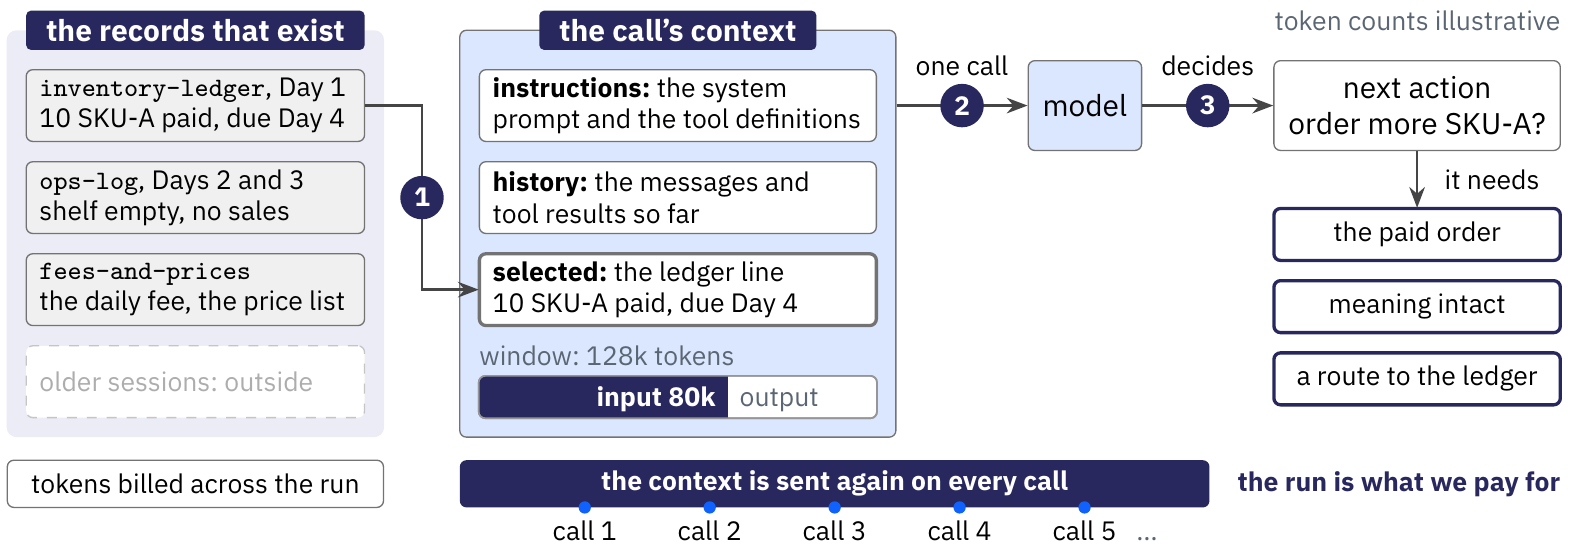
\includegraphics[width=\linewidth]{context/one-call-3.png}
\caption{Context supplies each call within a budget. The figure as it stands after the build's last click.}
\label{fig:one-call-3}
\end{figure}

\paragraph{The figure, stage by stage.}
\be
\item The call's context: arrow 1 selects the ledger line ``10 SKU-A paid, due Day 4'' from ``the records that exist'' and sets it beside the instructions and the history. The window meter shows ``input 80k'' of ``window: 128k tokens'', and the rest of the window is left for the ``output''.
\item The model: arrow 2, ``one call'', sends the context to the model, and arrow 3 shows what it ``decides'', the ``next action'', ``order more SKU-A?''. Under ``it needs'' stand the three things that decision requires from the context: ``the paid order'', ``meaning intact'' and ``a route to the ledger''.
\item The run meter: ``the context is sent again on every call'', from ``call 1'' to ``call 5'' and on, so the ``tokens billed across the run'' add up call after call. The verdict reads ``the run is what we pay for''.
\ee

\begin{takeaway}Context management fits what the next decision needs into the run's budget.\end{takeaway}

\subsection{Long-context research, from models to agents}
\label{sec:it-6-0}

\bi
\item \textbf{Models:} attention, positions and caches make windows longer and cheaper.
\item \textbf{Evaluations:} a model can use less of its window than its makers claim.
\item \textbf{Harnesses:} each call receives a context chosen for its decision.
\item \textbf{Agents:} long runs can produce more history than a window holds.
\ei

The budget of the previous slide has two answers in the research: make the window longer and cheaper, or choose what goes into it. The map places the work Part II builds on. Each lane collects the work that answers one question, and each runs left to right by first public release, the arXiv identifier or the date a test or post appeared. A work keeps the year it first appeared, so Lost in the Middle, which TACL published in 2024, sits at 2023. The reading list at the end of Part II gives every work with its venue and full reference.

The models lane asks how a model can attend to more tokens at lower cost. Transformer-XL (Dai et al., ACL 2019) carries hidden states across segments. Rotary position embedding (Su et al., arXiv 2021, Neurocomputing 2024) is the position scheme of most open models, and YaRN (Peng et al., ICLR 2024) stretches it to longer windows. FlashAttention (Dao et al., NeurIPS 2022) computes exact attention with memory linear in the input length. H2O (Zhang et al., NeurIPS 2023) and StreamingLLM (Xiao et al., ICLR 2024) evict entries from the key-value (KV) cache, the keys and values the model keeps for earlier tokens so that each new token need not recompute them, and the Gemini 1.5 report (Gemini Team, 2024) describes windows of a million tokens and more.

The evaluations lane asks how much of the window a model can use. Passkey retrieval (Mohtashami and Jaggi, NeurIPS 2023) and Needle In A Haystack (Kamradt, 2023, a test on GitHub) hide one fact in filler text. Lost in the Middle, the next slide, moves the evidence. RULER (Hsieh et al., COLM 2024) makes the tasks harder and finds that all but one of the 17 models it tested fall below a fixed score before their claimed length. Its two slides are backups at the end of Part II. HELMET (Yen et al., ICLR 2025) finds that needle scores predict application results poorly, and NoLiMa (Modarressi et al., ICML 2025) removes the literal overlap between the question and the needle, and scores fall.

The harnesses lane asks what each call should receive. RAG (Lewis et al., NeurIPS 2020) retrieves passages for each input. LLMLingua (Jiang et al., EMNLP 2023) and LLMLingua-2 (Pan et al., Findings of ACL 2024) keep the informative tokens. MemGPT (Packer et al., preprint, 2023) pages memory in and out of the window. SWE-agent (Yang et al., NeurIPS 2024) collapses old observations, The Complexity Trap (Lindenbauer et al., NeurIPS 2025 workshop) finds that such masking matches LLM summarization at lower cost, and ACON (Kang et al., ICML 2026) learns guidelines for compressing agent histories.

The agents lane asks what happens as runs grow long. SWE-bench (Jimenez et al., ICLR 2024) poses real GitHub issues in codebases far larger than a window. It is the standard testbed for coding agents, and two works of the harnesses lane, SWE-agent and The Complexity Trap, measure on it. A Vending-Bench run (Backlund and Petersson, preprint, 2025) lasts up to 2,000 messages and more than 20M tokens across its calls, while each call sees the last 30,000 tokens of its history. METR (Kwa et al., NeurIPS 2025) finds that the length of the tasks a model completes half the time, timed by human experts, has doubled about every seven months since 2019, and the long-horizon section draws its chart.

Part II takes the model as given and works in the harnesses lane, with evidence from the evaluations and agents lanes.

Every name on the map is a real work, placed at the year of its first public release, and nothing on it is illustrative. The lanes are the course's grouping: a work sits in the lane of the question it answers. SWE-agent chooses what each call receives, so it is a harness. SWE-bench, the coding agents' testbed, and Vending-Bench sit with the agents, and the evaluations lane holds the tests of one long input. The map shows 23 of the 59 works on the reading list and implies no ranking of influence.

\begin{figure}[htbp]
\centering
\includegraphics[width=\linewidth]{context/literature-map-5.png}
\caption{Long-context research, from models to agents The figure as it stands after the build's last click.}
\label{fig:literature-map-5}
\end{figure}

\paragraph{The figure, stage by stage.}
\be
\item Models, the first lane, in solid navy: Transformer-XL in 2019 carried state across segments, RoPE in 2021 set the position encoding that YaRN stretched in 2023, FlashAttention in 2022 made attention cheaper, H2O and StreamingLLM evict cached entries, and Gemini 1.5 reached a million tokens in 2024. The other three lane names wait in grey.
\item Evaluations: passkey retrieval and Needle In A Haystack hide one fact in filler text, Lost in the Middle moves the evidence, RULER makes the tasks harder, HELMET tests application tasks, and NoLiMa removes the literal overlap between the question and the needle. The window a maker claims and the length a model can use come apart. The models lane settles to lilac.
\item Harnesses: RAG retrieves, LLMLingua and LLMLingua-2 extract, MemGPT pages memory, SWE-agent masks old observations, and the Complexity Trap and ACON measure and learn compression for agents. Each chooses what a call receives. The evaluations lane settles.
\item Agents: SWE-bench sets real GitHub issues in codebases far larger than a window, the testbed of the harness studies. A Vending-Bench run lasts up to 2,000 messages and more than 20M tokens across its calls, while each call sees the last 30,000 tokens of its history. METR's time horizon, the length of task, timed by human experts, that a model completes half the time, has doubled about every seven months. The harnesses lane settles.
\item The four works in navy each have a slide of their own in Part II: Lost in the Middle next, LLMLingua-2 in the strategies segment, and METR's time horizons and Vending-Bench in the long-horizon segment. The rest of the agents lane settles. Part II works in the harnesses lane, with evidence from the evaluations and agents lanes.
\ee

\begin{takeaway}Longer windows still leave each call's context to the harness.\end{takeaway}

\subsection{Evidence position changes accuracy}
\label{sec:it-6-1}

\bi
\item \textbf{Lost in the Middle} (Liu et al., 2024) moves the answer among 20 documents.
\item \textbf{The reported pattern:} accuracy is often highest with the answer first or last, and lowest in the middle.
\item \textbf{The scope:} the models and tasks tested. A present system needs its own test.
\ei

Nelson F. Liu, Kevin Lin, John Hewitt, Ashwin Paranjape, Michele Bevilacqua, Fabio Petroni and Percy Liang, Lost in the Middle: How Language Models Use Long Contexts, Transactions of the Association for Computational Linguistics 12, 157--173, 2024 (doi:10.1162/tacl\_a\_00638). This is one of the sources Part II studies in depth, and the navy work in the evaluations lane of the map on the slide \hyperref[sec:it-6-0]{``Long-context research, from models to agents''}. RULER, its companion, is a backup at the end of Part II. SWE-bench met the same effect on real software tasks: models resolved fewer issues as the retrieved context grew, and its authors cite this paper for it (Jimenez et al., ICLR 2024, section 5).

The study varies the position of the relevant information in multi-document question answering and in key-value retrieval. Performance is often strongest when the relevant information sits near the start or the end of the input, and weaker when it sits in the middle. The finding concerns the models, prompts and tasks the study evaluated, so we do not carry its numbers to current models. A present system needs its own measurement. The open-domain question-answering case study also separates retriever recall from reader accuracy: added retrieved material need not give proportional gains in the answers.

The figure draws the shape of the finding and no values. Its question about Day 4 is the course's example, and its 20 documents are one of the paper's multi-document settings, which also ran 10 and 30 documents with questions from NaturalQuestions-Open. The key-value retrieval task is not drawn. Both ends carry the label ``accuracy high'', which does not mean that they score the same. The result holds for the models and prompts the paper tested in 2023, and no number carries over to current models.

\begin{figure}[htbp]
\centering
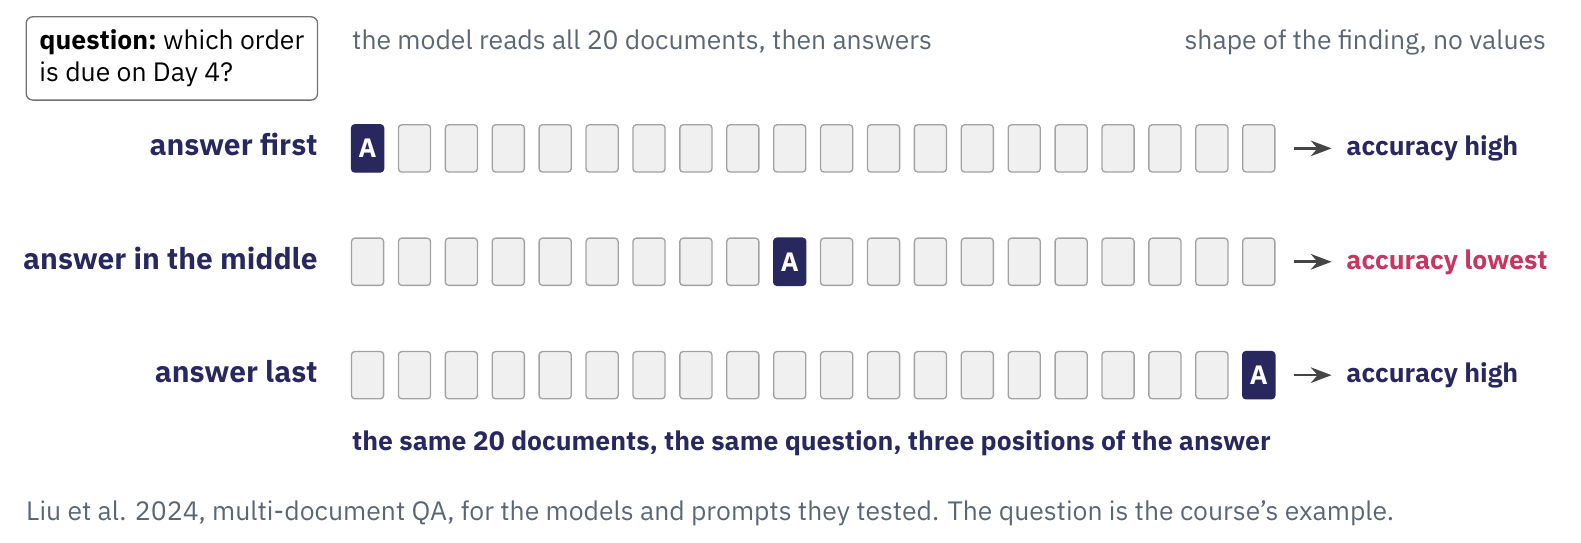
\includegraphics[width=\linewidth]{context/evidence-position-3.png}
\caption{Evidence position changes accuracy. The figure as it stands after the build's last click.}
\label{fig:evidence-position-3}
\end{figure}

\paragraph{The figure, stage by stage.}
\be
\item Answer first: the document marked A holds the answer to 'which order is due on Day 4?' and comes first of the 20. The model reads all 20 documents, then answers, and Liu et al. report accuracy high at this position.
\item Answer in the middle: the same answer document moves to position 10 of the 20. The magenta verdict, accuracy lowest, marks the position where the models and prompts Liu et al. tested answer least accurately.
\item Answer last: the answer document moves to position 20, and the verdict reads accuracy high again. The caption names what stays fixed: the same 20 documents, the same question, three positions of the answer.
\ee

\begin{takeaway}Where evidence sits in the input is a variable each system must test.\end{takeaway}

\subsection*{Key points}
\bi
\item Part II asks what each call must see so that the run keeps its commitments.
\item Context management fits what the next decision needs into the run's budget.
\item Longer windows still leave each call's context to the harness.
\item Where evidence sits in the input is a variable each system must test.
\ei

\section{Strategies and harness formats}
\label{sec:row-1}

The experiment shows that a model can use a long input unevenly, so we turn to the harnesses lane of the map, how a harness chooses what each call receives: the ways to manage context, one measured method of extraction, the abstractive rewriting that harnesses use, the methods learned for agents since 2025, the compaction strategies one by one, the formats of Pi, Claude Code and Codex, and the tools LangGraph supplies.

\subsection{Context: retain, retrieve, extract, rewrite}
\label{sec:it-7-1}

\bi
\item \textbf{Retain} keeps selected original messages or results.
\item \textbf{Retrieve} fetches material by query or reference when needed.
\item \textbf{Extract} keeps only the informative tokens of what stays.
\item \textbf{Rewrite} replaces a span with a generated summary.
\ei

These four ways are the course's organizing scheme for Part II. Retain keeps original messages or results as they were written. Retrieve fetches material by query or by reference when it is needed. Extract keeps only the informative tokens of what stays. Rewrite replaces a span with a generated summary. Retrieval draws on a large literature, such as retrieval-augmented generation (Lewis et al., Retrieval-Augmented Generation for Knowledge-Intensive NLP Tasks, NeurIPS 2020), which stays supporting reading. The four ways also sort the harnesses lane of the map: RAG retrieves, LLMLingua and LLMLingua-2 extract, MemGPT retrieves and rewrites, SWE-agent retains its latest observations whole, and ACON rewrites. The next slides open extraction and rewriting, then compare the compaction strategies one by one.

The ledger line and its four forms are illustrative. The extract row drops only the colon and the two commas, shown in grey, a small instance of the keep-or-drop choice that LLMLingua-2's classifier makes for every word. The rewrite row says the same facts in fewer, new words. The four-way split is the course's scheme, attributed to no paper.

\begin{figure}[htbp]
\centering
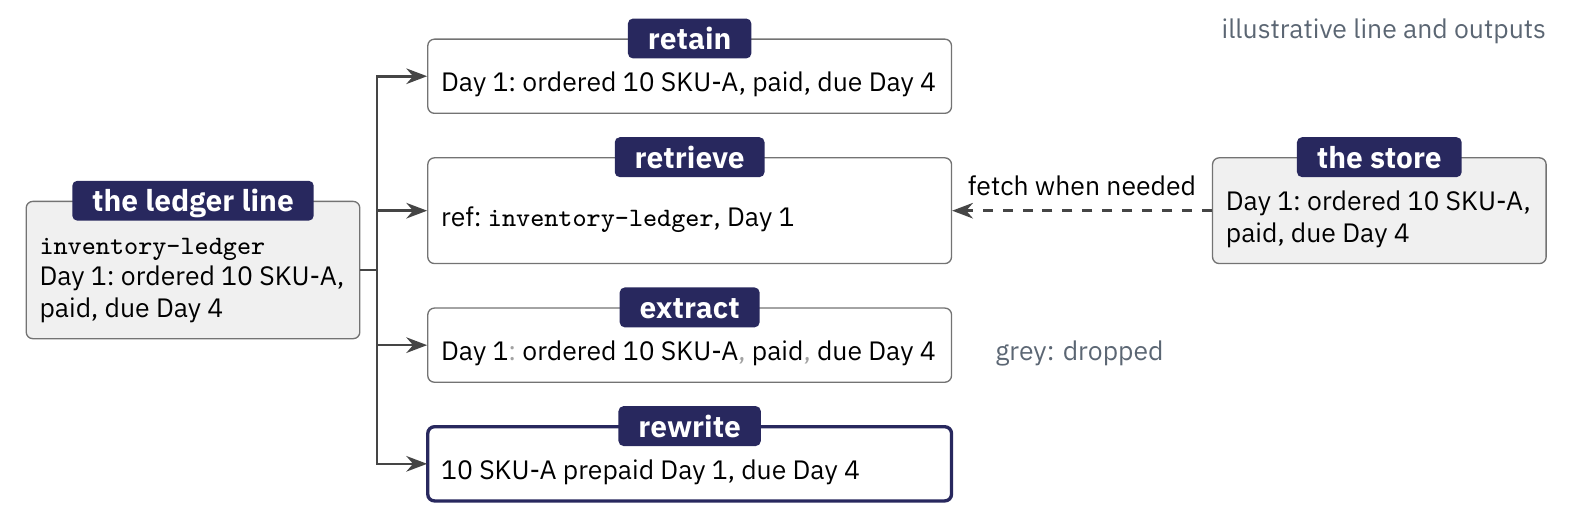
\includegraphics[width=\linewidth]{context/four-ways-4.png}
\caption{Context: retain, retrieve, extract, rewrite The figure as it stands after the build's last click.}
\label{fig:four-ways-4}
\end{figure}

\paragraph{The figure, stage by stage.}
\be
\item Retain: the later call receives the ledger line from inventory-ledger word for word, Day 1: ordered 10 SKU-A, paid, due Day 4. The order, the payment and the due date all reach the call.
\item Retrieve: the context carries only the reference ref: inventory-ledger, Day 1, and the line itself stays in the store. The dashed arrow, fetch when needed, brings the line back when a later call asks for it.
\item Extract: the row keeps every word of the ledger line in its order. The colon and the two commas are dropped, and the key grey: dropped marks them.
\item Rewrite: the new sentence 10 SKU-A prepaid Day 1, due Day 4 keeps every fact in fewer words, so its box is shorter than the line's. The word prepaid never appears in the ledger line, which shows that the sentence is generated.
\ee

\begin{takeaway}A context policy determines what to keep, fetch, shorten or rewrite.\end{takeaway}

\subsection{Extractive compression selects tokens}
\label{sec:it-7-2}

\bi
\item \textbf{LLMLingua-2} (Pan et al., 2024) trains a classifier to keep or drop each token.
\item \textbf{The method:} trained on GPT-4's compressions, it reads both sides of a token.
\item \textbf{The evaluation:} task scores, compression and latency on several datasets.
\ei

Zhuoshi Pan et al., LLMLingua-2: Data Distillation for Efficient and Faithful Task-Agnostic Prompt Compression, Findings of ACL 2024, 963--981 (doi:10.18653/v1/2024.findings-acl.57). This is the navy work of the map's harnesses lane, the mechanism Part II studies in depth. Its origin is LLMLingua (Jiang et al., LLMLingua: Compressing Prompts for Accelerated Inference of Large Language Models, EMNLP 2023), and LongLLMLingua (Jiang et al., LongLLMLingua: Accelerating and Enhancing LLMs in Long Context Scenarios via Prompt Compression, ACL 2024) is its long-context extension.

LLMLingua-2 trains a token classifier on an extractive compression dataset distilled from GPT-4. GPT-4 compresses MeetingBank transcripts, in chunks of at most 512 tokens, by deleting words, and an alignment algorithm turns each compression into a keep or drop label for every original word (section 3.2). The classifier uses the context on both sides of each token to decide whether to keep it. The evaluations compare compression with task scores and latency on MeetingBank and on out-of-domain datasets. The reported gains apply to those test conditions, so we promise no fixed compression ratio or speed-up.

The limit, which the slide \hyperref[sec:it-7-4b]{``Extractive selection keeps key tokens.''} shows, is that deleting tokens can lose the meaning the task needs, so we test every use on the task. Inside agents the loss is measured: the slide \hyperref[sec:it-7-3b]{``Agents now learn what their context keeps.''} follows the work since 2025 that compacts an agent's history instead of its words.

The line ``ordered 10 SKU-A, paid, due Day 4 unless cancelled'' extends the deck's running ledger line for this slide, and its keep and drop labels are the course's example. LLMLingua-2's classifier did not produce them. The paper distills its training data from GPT-4.

\begin{figure}[htbp]
\centering
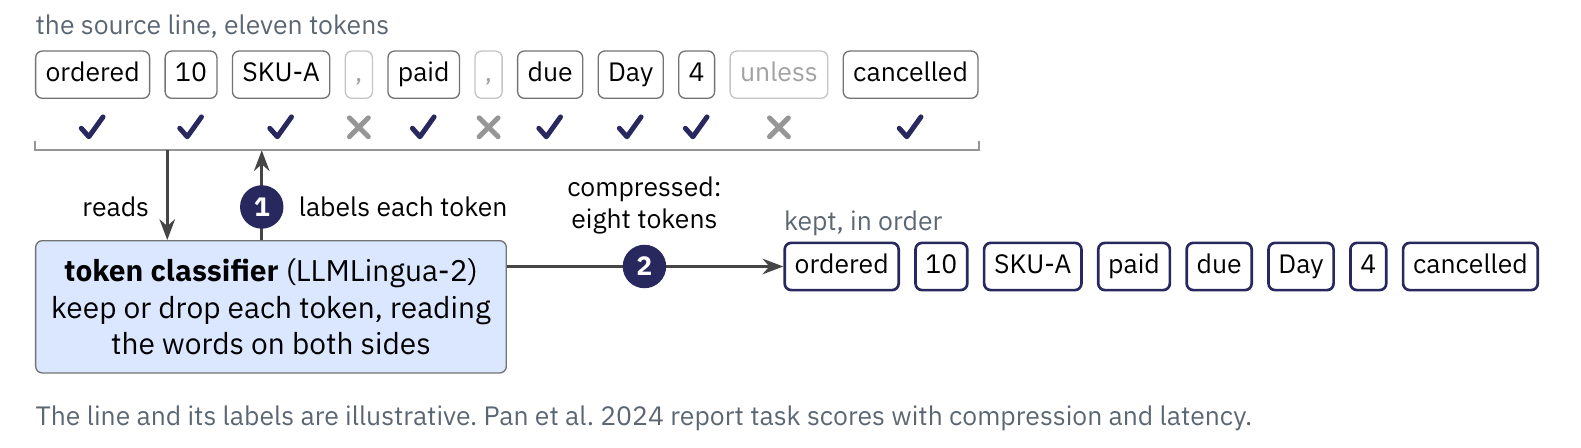
\includegraphics[width=\linewidth]{context/extractive-3.png}
\caption{Extractive compression selects tokens. The figure as it stands after the build's last click.}
\label{fig:extractive-3}
\end{figure}

\paragraph{The figure, stage by stage.}
\be
\item The source line, eleven tokens: ordered, 10, SKU-A, a comma, paid, a comma, due, Day, 4, unless and cancelled. As written, the order stands unless someone cancels it, and the dashed box marks where the token classifier will stand.
\item The token classifier (LLMLingua-2) reads the line, and arrow 1, 'labels each token', marks every token keep or drop, reading the words on both sides. Eight tokens get a navy tick, and the two commas and unless get a grey cross.
\item Arrow 2, 'compressed: eight tokens', leads to the row 'kept, in order': ordered, 10, SKU-A, paid, due, Day, 4 and cancelled. The two commas and unless fade in the source line because the next call never receives them.
\ee

\begin{takeaway}A compressed input is judged by the task it must support.\end{takeaway}

\subsection{Abstractive compaction rewrites history}
\label{sec:it-7-3}

\bi
\item \textbf{Input:} selected conversation history or observations.
\item \textbf{Transformation:} a model summarizes what the next step needs.
\item \textbf{Replacement:} later calls carry the summary plus retained material.
\item \textbf{Risk:} omissions and unsupported claims change what the next call believes.
\ei

Abstractive compaction takes selected history or observations, has a model write a shorter summary of the information the next step needs, and assembles later requests from that summary plus any material kept on purpose. An omission or an unsupported statement in the summary changes what the next call believes.

The article of Anthropic's Applied AI team (Effective context engineering for AI agents, September 29, 2025) describes compaction as a summary that replaces the history in a fresh context. Its compaction section warns that overly aggressive compaction can lose context whose importance appears only later, and it recommends tuning the summary prompt on complex agent traces. This is engineering guidance rather than a controlled comparison. The course groups the methods as retain, retrieve, extract and rewrite, and the long-horizon example uses abstractive compaction.

The five messages stand for a longer history, and the token counts are illustrative. The next request's three parts (the system prompt, the summary, the recent messages) follow Pi's documented rebuild. No stage shows an unsupported statement, and the faithfulness check of the evaluation section returns to that half of the risk.

\begin{figure}[htbp]
\centering
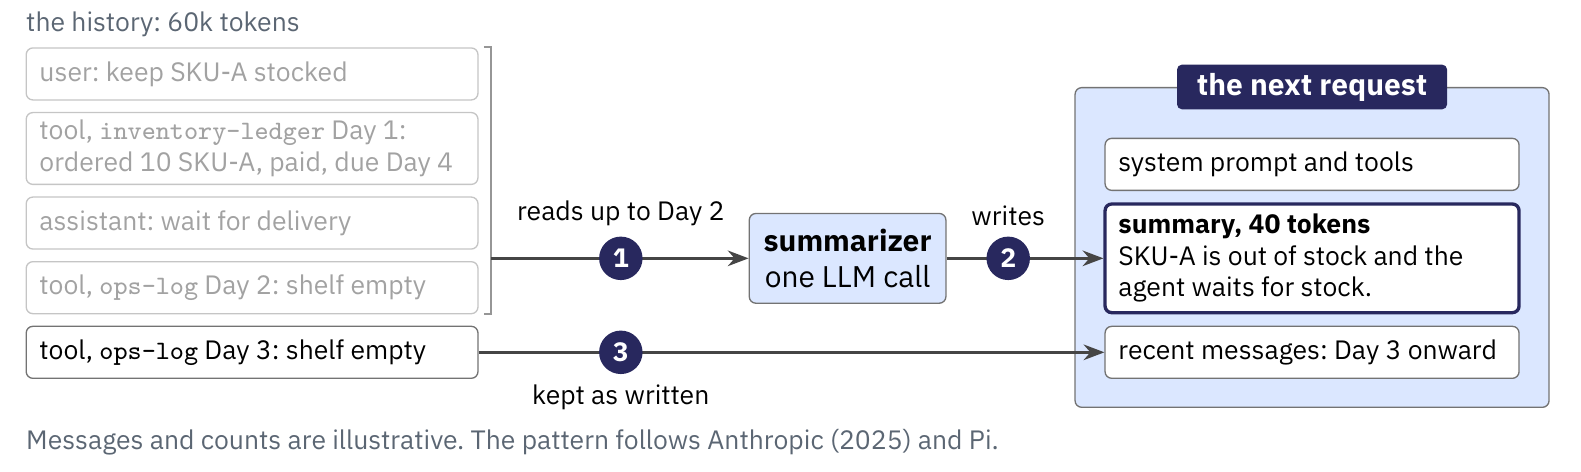
\includegraphics[width=\linewidth]{context/abstractive-3.png}
\caption{Abstractive compaction rewrites history. The figure as it stands after the build's last click.}
\label{fig:abstractive-3}
\end{figure}

\paragraph{The figure, stage by stage.}
\be
\item The history: 60k tokens in five messages, from 'user: keep SKU-A stocked' and 'tool, inventory-ledger Day 1: ordered 10 SKU-A, paid, due Day 4' to the two ops-log lines 'shelf empty' on Days 2 and 3. The dashed box marks where the summarizer will stand.
\item The summarizer, one LLM call, reads up to Day 2 and writes 'summary, 40 tokens: SKU-A is out of stock and the agent waits for stock.' The four messages it read fade because the next call will not receive them, and the Day 3 log stays dark.
\item The next request holds 'system prompt and tools', the summary and 'recent messages: Day 3 onward'. Arrow 3 carries the Day 3 log into it, kept as written.
\ee

\begin{takeaway}A generated summary becomes another representation that needs checking.\end{takeaway}

\subsection{Agents now learn what their context keeps}
\label{sec:it-7-3b}

\bi
\item \textbf{Token pruning:} deleting words inside an agent's messages cost 17 points.
\item \textbf{Masking:} a rule replaces old tool observations with placeholders.
\item \textbf{Learned guidelines:} a compressor follows instructions refined on failed runs.
\item \textbf{Trained folding:} the agent learns by RL to fold each finished subtask.
\ei

LLMLingua-2 compresses one prompt for any task. Since 2025, compaction research has turned to agents, whose histories grow with every tool call, and it has moved the decision about what to drop from a fixed rule to a tuned compressor and then to the agent's own trained policy. Each row of the figure is one step, with a result that its paper compares against the same model with the full history.

Token pruning inside an agent: ACON (Minki Kang and colleagues, ACON: Optimizing Context Compression for Long-horizon LLM Agents, ICML 2026, arXiv:2510.00615) includes an LLMLingua baseline. On AppWorld with gpt-4.1, accuracy falls from 56.0\% with the full history to 39.3\%. SWE-Pruner (Wang and colleagues, a 2026 preprint) reports the same direction on 50 tasks of SWE-bench Verified: LLMLingua-2 takes success from 62\% to 54\%.

Masking: The Complexity Trap (Tobias Lindenbauer and colleagues, DL4C workshop at NeurIPS 2025, arXiv:2508.21433) replaces every tool observation older than the last ten turns with a placeholder and keeps all reasoning and actions. With Qwen3-Coder 480B in SWE-agent on SWE-bench Verified, masking solves 54.8\% of the tasks at \$0.61 each, an LLM summary 53.8\% at \$0.64, and the raw history 53.4\% at \$1.29. Observations make up about 84\% of a turn's tokens, which is why masking saves so much. It is the agent's version of keeping the recent turns, and LangGraph's ClearToolUsesEdit and Anthropic's context editing implement it.

Learned guidelines: ACON compresses the history, or one long observation, with an LLM that follows written guidelines. An optimizer LLM refines the guidelines from runs that succeed without compression and fail with it, and the compressor is then distilled into a small model. On AppWorld with gpt-4.1, accuracy is 56.5\% against 56.0\% without compression, while the peak context falls from 9.93K to 7.33K tokens. Across its benchmarks, peak tokens fall by 26 to 54\%.

Trained folding: Context-Folding (Weiwei Sun and colleagues, Scaling Long-Horizon Agent via Context Folding, ICML 2026, arXiv:2510.11967) trains the agent with reinforcement learning (FoldGRPO) to branch into a subtask and fold it into one summary when the subtask ends. Seed-OSS-36B with a 32K active context reaches 58.0\% on SWE-bench Verified and 62.0\% on BrowseComp-Plus, against 57.4\% and 54.0\% for an RL-trained ReAct agent with a 327K window. MEM1 (Zhou and colleagues, ICLR 2026) and AgentFold (Ye and colleagues, ICLR 2026) train similar policies.

The vendors have built the last step into their models and APIs. OpenAI describes GPT-5.1-Codex-Max (November 19, 2025) as natively trained to work across context windows through compaction, its Responses API compacts on request or on the server, and the Claude API has compacted on the server since February 5, 2026.

The six turns, the block widths and the turns each method changes are illustrative: the paper's masking keeps the last ten turns where the figure keeps two. Each row's numbers come from its own benchmark and models, as the note under the figure says, so they compare only within a row. ACON's LLMLingua baseline does not name its checkpoint.

\begin{figure}[htbp]
\centering
\includegraphics[width=\linewidth]{context/agent-compaction-5.png}
\caption{Agents now learn what their context keeps. The figure as it stands after the build's last click.}
\label{fig:agent-compaction-5}
\end{figure}

\paragraph{The figure, stage by stage.}
\be
\item The history: six turns of an agent, each a short action in blue and a wide tool observation in grey. Observations are about 84\% of a turn's tokens, the share The Complexity Trap measured in SWE-agent. The grey note says that each row's numbers come from its own benchmark.
\item Token pruning: words are deleted inside every message, as LLMLingua does. Inside an agent, ACON's LLMLingua baseline falls from 56.0\% with the full history to 39.3\% on AppWorld.
\item Masking: a rule replaces the old observations with short placeholders and keeps every action. On SWE-bench Verified, masking solves 54.8\%, 52\% cheaper than the raw history.
\item Learned guidelines: a compressor rewrites the old turns into one summary, following guidelines learned from failed runs. ACON keeps AppWorld at 56.5\% while the peak context falls 26\%.
\item Trained folding: the agent itself, trained by reinforcement learning, folds a finished subtask into one summary. Context-Folding reaches 58.0\% on SWE-bench Verified with 32K of context, against 57.4\% with 327K.
\ee

\begin{takeaway}Newer compaction is measured, and often trained, on the agent's own tasks.\end{takeaway}

\subsection{Recency keeps the last turns}
\label{sec:it-7-4a}

\bi
\item \textbf{How:} the harness keeps the most recent turns and drops older ones.
\item \textbf{Strength:} no extra call and no extra tokens.
\item \textbf{Failure:} an old but open commitment is dropped.
\ei

Recency keeps the most recent turns and drops the older ones, so it costs nothing beyond the drop. Its failure is an old commitment that is still open: the order paid on Day 1 leaves the context while its delivery is still due. Recency is the fallback when nothing else is in place, and Pi keeps the most recent messages beside its summary (the slide \hyperref[sec:it-7-5a]{``Pi compacts into a structured summary.''}).

Agent harnesses apply the same idea to tool results. SWE-agent (Yang et al., NeurIPS 2024) keeps the last five observations whole and collapses each older one to a single line. The Complexity Trap (Lindenbauer et al., NeurIPS 2025 workshop) compared the same masking, keeping the observations of the last ten turns, against LLM summarization on SWE-bench Verified: masking halved the cost of the unmanaged agent and matched the solve rate of summarization. Masking collapses old tool output and keeps every thought and action, so a commitment the agent wrote down stays in the context (SWE-agent keeps the agent's plan and actions, Yang et al., section 3). The figure's recency drops whole turns, actions included. A solve rate on SWE-bench Verified does not show whether an old open commitment survived.

The eight turns and the context of the last five are illustrative. Pi sizes its kept messages in tokens (keepRecentTokens, 20k tokens by default) where the figure counts turns, and ``the cheapest strategy'' is the course's comparison rather than a measurement.

\begin{figure}[htbp]
\centering
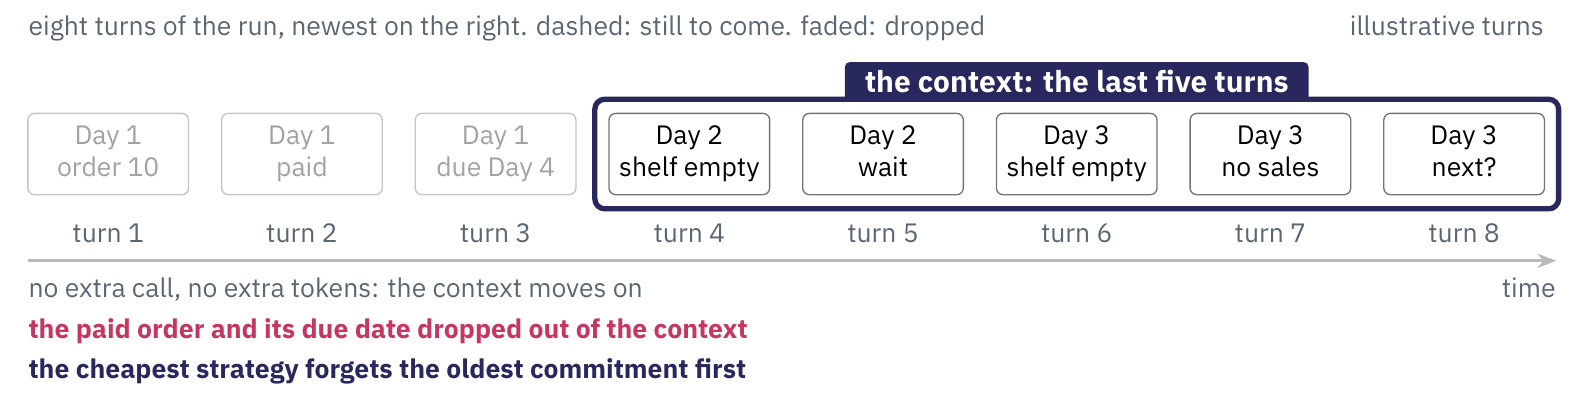
\includegraphics[width=\linewidth]{context/recency-3.png}
\caption{Recency keeps the last turns. The figure as it stands after the build's last click.}
\label{fig:recency-3}
\end{figure}

\paragraph{The figure, stage by stage.}
\be
\item The context: the last five turns holds turns 1 to 5, and turns 1 to 3 carry order 10, paid and due Day 4 from Day 1. The dashed turns 6 to 8 are still to come.
\item The context moves on to turns 3 to 7, and turns 1 and 2, order 10 and paid, fade as dropped. The note gives the cost: no extra call, no extra tokens: the context moves on.
\item The context moves again to turns 4 to 8, and turn 3, due Day 4, fades. The magenta line names the loss, the paid order and its due date dropped out of the context, and the navy line gives the verdict, the cheapest strategy forgets the oldest commitment first.
\ee

\begin{takeaway}Recency adds no cost, and an open commitment leaves with its old turns.\end{takeaway}

\subsection{Extractive selection keeps key tokens}
\label{sec:it-7-4b}

\bi
\item \textbf{How:} a classifier keeps the informative tokens and drops the rest.
\item \textbf{Strength:} cheap and model-agnostic.
\item \textbf{Failure:} one dropped word can flip the meaning.
\ei

Extractive selection keeps the informative tokens and drops the rest, so it is cheap and works with any downstream model. The kept tokens read as a terse excerpt of the source. One dropped word can flip the meaning, which is why the compressed input is tested on the task. LLMLingua-2 (the slide \hyperref[sec:it-7-2]{``Extractive compression selects tokens.''}) is the worked method.

The dropped ``unless'' is the course's example. The strength follows from the method: a small classifier runs once over the input, and any model can read the kept tokens.

\begin{figure}[htbp]
\centering
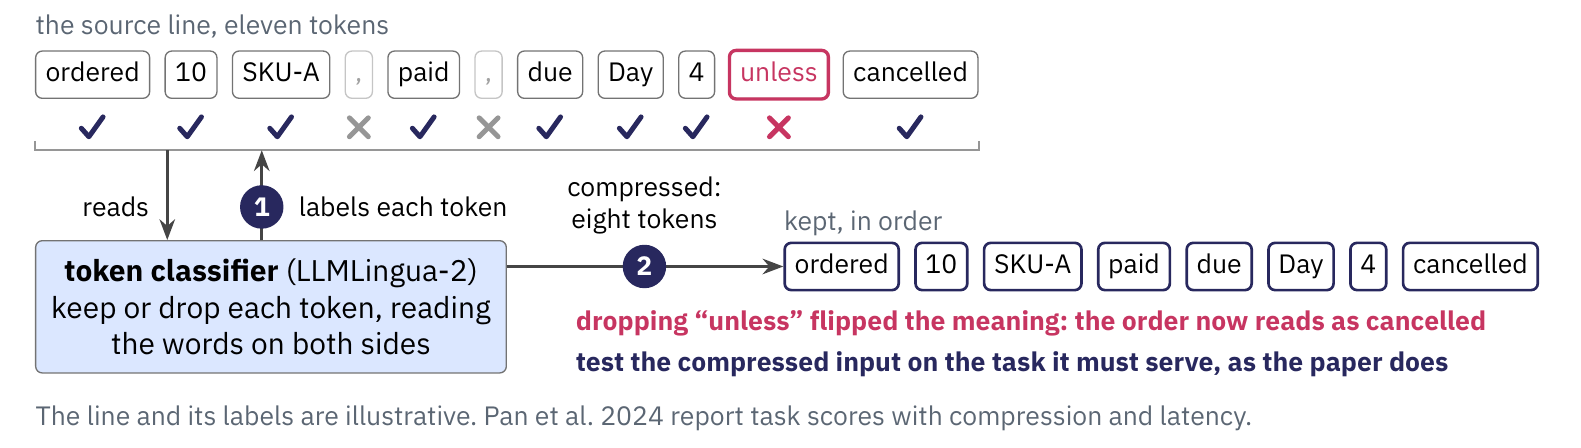
\includegraphics[width=\linewidth]{context/extractive-4.png}
\caption{Extractive selection keeps key tokens. The figure as it stands after the build's last click.}
\label{fig:extractive-4}
\end{figure}

\paragraph{The figure, stage by stage.}
\be
\item Arrow 2, 'compressed: eight tokens', leads to the row 'kept, in order': ordered, 10, SKU-A, paid, due, Day, 4 and cancelled. The two commas and unless fade in the source line because the next call never receives them.
\item The dropped word unless turns magenta, and so does its cross. The magenta line reads 'dropping ``unless'' flipped the meaning: the order now reads as cancelled', and the navy line names the check: 'test the compressed input on the task it must serve, as the paper does'.
\ee

\begin{takeaway}Extraction shortens the text and keeps the original words.\end{takeaway}

\subsection{Abstractive summary rewrites a span}
\label{sec:it-7-4c}

\bi
\item \textbf{How:} an LLM writes a shorter summary of a span of history.
\item \textbf{Strength:} it preserves meaning flexibly.
\item \textbf{Failure:} omission and unsupported claims.
\ei

An LLM writes a shorter summary of a span, which preserves the meaning flexibly. The summary can omit a fact or state one that the history does not support. This summary is the core of every harness format later in this section, and it becomes a new representation to verify.

The title rests on the Anthropic Applied AI team's Effective context engineering for AI agents (September 29, 2025, engineering guidance), whose compaction section describes summarizing a conversation near the window limit and starting a new context with the summary (the slide \hyperref[sec:it-7-3]{``Abstractive compaction rewrites history.''}). Pi summarizes its older messages with an LLM, and the next request in the figure follows its documented rebuild (the slide \hyperref[sec:it-7-5a]{``Pi compacts into a structured summary.''}).

MemGPT (Packer et al., preprint, 2023) keeps a recursive summary of the messages it evicts from the window. Repeated rewriting carries its own risk: Agentic Context Engineering (Zhang et al., ICLR 2026) describes context collapse, in which iterative rewriting erodes details over time.

The omitted order is the course's example, and the summary's wording is illustrative.

\begin{figure}[htbp]
\centering
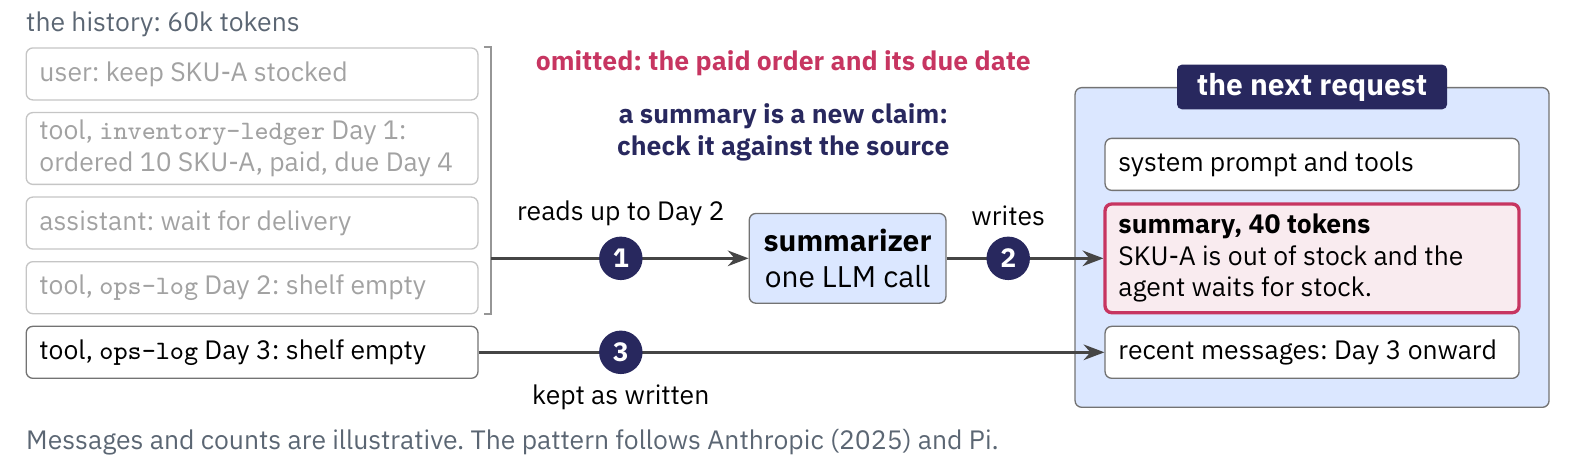
\includegraphics[width=\linewidth]{context/abstractive-4.png}
\caption{Abstractive summary rewrites a span. The figure as it stands after the build's last click.}
\label{fig:abstractive-4}
\end{figure}

\paragraph{The figure, stage by stage.}
\be
\item The next request holds 'system prompt and tools', the summary and 'recent messages: Day 3 onward'. Arrow 3 carries the Day 3 log into it, kept as written.
\item The summary turns magenta, and the magenta line names what it lost: 'omitted: the paid order and its due date'. The navy line names the check: 'a summary is a new claim: check it against the source'.
\ee

\begin{takeaway}A summary restates meaning in new words and needs checking.\end{takeaway}

\subsection{Structured notes hold a running state}
\label{sec:it-7-4d}

\bi
\item \textbf{How:} each step updates a card of goals, open items and decisions.
\item \textbf{Strength:} commitments survive by design.
\item \textbf{Failure:} a fact the schema has no field for is lost.
\ei

Structured notes keep a schema of goals, open items and decisions that each step updates, so a commitment written into the card survives by design. The schema must anticipate what matters: a fact with no field, such as the supplier's warning, has no place to go. Pi uses fixed summary sections and file lists as structured notes (the slide \hyperref[sec:it-7-5a]{``Pi compacts into a structured summary.''}), and Codex can also keep structured memory across sessions when its memories feature is on (the slide ``Codex's local path writes a handoff summary.'').

The card's fields and entries are illustrative. Pi refreshes its fixed sections at each compaction, so a card written at every step is the strategy's idealized form. The failure, a fact with no field, is the course's reasoning, and no source measures how often it happens.

\begin{figure}[htbp]
\centering
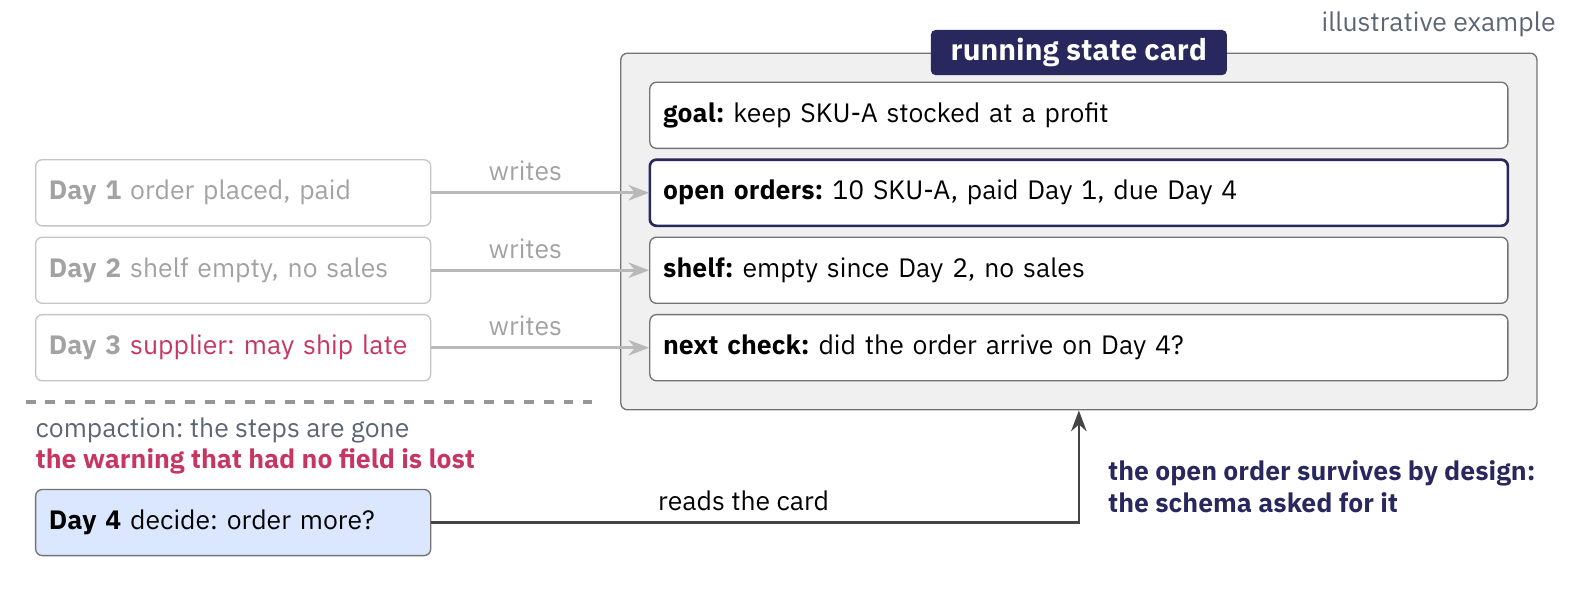
\includegraphics[width=\linewidth]{context/structured-notes-3.png}
\caption{Structured notes hold a running state. The figure as it stands after the build's last click.}
\label{fig:structured-notes-3}
\end{figure}

\paragraph{The figure, stage by stage.}
\be
\item The running state card holds four fields: 'goal: keep SKU-A stocked at a profit', 'open orders: 10 SKU-A, paid Day 1, due Day 4', and two ghosts, 'shelf: none yet' and 'next check: none yet'. The step 'Day 1 order placed, paid' writes the open order into its field.
\item Days 2 and 3 fill the two ghosts: 'Day 2 shelf empty, no sales' writes 'shelf: empty since Day 2, no sales', and 'Day 3 supplier: may ship late' writes 'next check: did the order arrive on Day 4?'. The card has no field for the supplier's warning itself, and the open-orders line stays as Day 1 wrote it.
\item Compaction arrives as a grey dashed rule, 'compaction: the steps are gone', and 'Day 4 decide: order more?' 'reads the card'. In magenta, 'the warning that had no field is lost'. The open-orders field takes a navy outline, and the navy line under the card, where Day 4's arrow enters it, reads 'the open order survives by design: the schema asked for it'.
\ee

\begin{takeaway}A running state card carries commitments across every compaction.\end{takeaway}

\subsection{Sub-agent delegation isolates a context}
\label{sec:it-7-4e}

\bi
\item \textbf{How:} a sub-agent runs a subtask in its own context and returns one result.
\item \textbf{Strength:} the main context stays small.
\item \textbf{Failure:} the result can omit a fact the main agent needs.
\ei

Delegation runs a subtask in its own context and returns one result, so the main context grows by the result alone. The result is lossy: it can omit a fact the main agent needs, such as the supplier's warning, while the sub-agent's reads stay in its own context. Claude Code uses subagents this way (the slide \hyperref[sec:it-7-5b]{``Claude Code summarizes and re-reads files.''}), and the main agent sees the result rather than the subtask's reads.

The token counts and sizes are illustrative, and the short result is a simplification. Claude Code's documentation says that subagents keep large reads outside the main context, and QwenGyre (Wang et al., preprint, 2026, on the slide \hyperref[sec:it-7-5]{``Real harnesses compact, delegate and retry.''}) describes sub-agents with separate contexts. Neither gives sizes or a loss rate, so the loss is a design risk.

\begin{figure}[htbp]
\centering
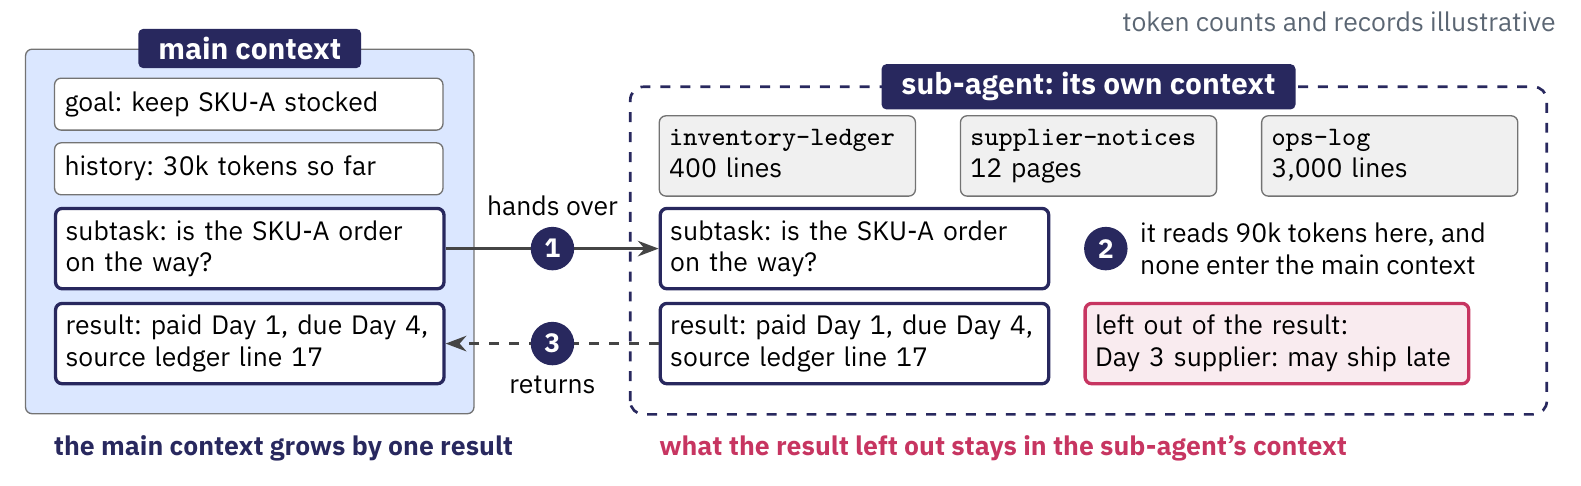
\includegraphics[width=\linewidth]{context/delegation-3.png}
\caption{Sub-agent delegation isolates a context. The figure as it stands after the build's last click.}
\label{fig:delegation-3}
\end{figure}

\paragraph{The figure, stage by stage.}
\be
\item The main context holds 'goal: keep SKU-A stocked', 'history: 30k tokens so far' and the subtask 'is the SKU-A order on the way?'. Event 1 'hands over' the subtask to a sub-agent that works in its own context, and two ghosts marked 'result' show where the answer will go.
\item Three records arrive in the sub-agent's context: inventory-ledger (400 lines), supplier-notices (12 pages) and ops-log (3,000 lines), about 8k, 7k and 75k tokens. Event 2 says 'it reads 90k tokens here, and none enter the main context'.
\item Event 3 'returns' one result, 'result: paid Day 1, due Day 4, source ledger line 17', so 'the main context grows by one result'. The magenta chip 'left out of the result: Day 3 supplier: may ship late' shows that 'what the result left out stays in the sub-agent's context'.
\ee

\begin{takeaway}Delegation moves a subtask's reads out of the main context.\end{takeaway}

\subsection{Retrieval keeps records outside the context}
\label{sec:it-7-4f}

\bi
\item \textbf{How:} records stay in a store outside the context, behind a reference.
\item \textbf{Strength:} it scales past any window.
\item \textbf{Failure:} a query miss or a stale reference.
\ei

Retrieval keeps records in a store outside the context and fetches them by reference when they are needed, so it scales past any window. It fails when a query misses or when a reference has gone stale. Claude Code's re-read of recently touched files after compaction is a bounded form (the slide \hyperref[sec:it-7-5b]{``Claude Code summarizes and re-reads files.''}), and retrieval-augmented generation is the general case. Xu et al. (Retrieval meets Long Context Large Language Models, ICLR 2024) compare the map's two answers directly, a longer window against retrieval: a model with a 4K window and retrieval matched one fine-tuned to a 16K window, and retrieval still helped models with 32K windows.

The store, its line numbers, the cleanup and the counts are illustrative, and the stale reference is a constructed case. The query miss is not drawn. Retrieval scales past any window because the store sits outside it.

\begin{figure}[htbp]
\centering
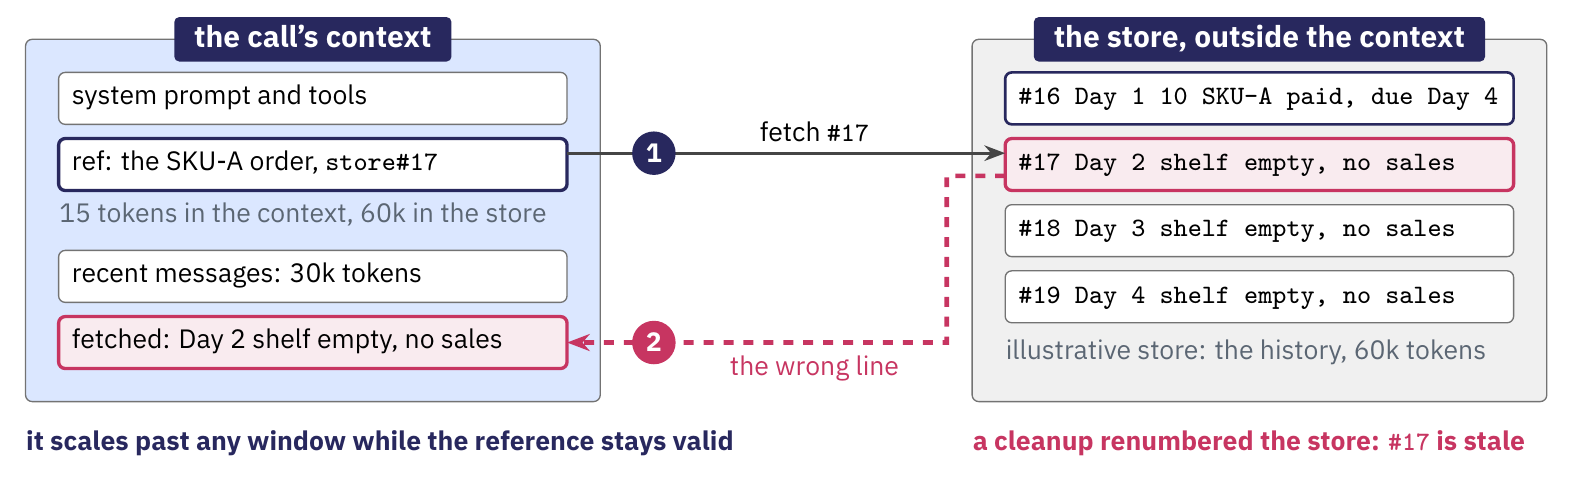
\includegraphics[width=\linewidth]{context/retrieval-3.png}
\caption{Retrieval keeps records outside the context. The figure as it stands after the build's last click.}
\label{fig:retrieval-3}
\end{figure}

\paragraph{The figure, stage by stage.}
\be
\item The call's context keeps a reference where the line would be, ref: the SKU-A order, store\#17, at 15 tokens in the context, 60k in the store. The store, outside the context, holds the history with the paid order at \#17, and the ghost marks where the fetched line will go.
\item Fetch \#17 reaches row \#17, and the line comes back word for word as fetched: Day 1 10 SKU-A paid, due Day 4. The paid order enters the context when the decision needs it.
\item A cleanup renumbered the store: \#17 is stale, so the same fetch returns the wrong line, Day 2 shelf empty, no sales, while the paid order sits at \#16. The navy line states the condition: it scales past any window while the reference stays valid.
\ee

\begin{takeaway}Retrieval trades in-context text for a fetch when it is needed.\end{takeaway}

\subsection{Compaction strategies compared}
\label{sec:it-7-4g}

\textbf{This table recaps the strategies of the previous slides.}

This table recaps the six strategy slides, one row per click. Each strategy buys room by giving up a different kind of recall: recency the oldest commitment, extraction the words it drops, a summary what it omits, structured notes what the schema has no field for, delegation what the result leaves out, and retrieval what a query misses.

The strategies use the four ways of the slide \hyperref[sec:it-7-1]{``Context: retain, retrieve, extract, rewrite''}. Recency retains the newest turns as written, extractive selection extracts, an abstractive summary rewrites, and structured notes rewrite the run's state into fields. Retrieval on demand is the retrieve way, and delegation moves a subtask's reads into a context of its own.

KV-cache eviction works at a different layer, the models lane of the map. StreamingLLM (Xiao et al., Efficient Streaming Language Models with Attention Sinks, ICLR 2024) and H2O (Zhang et al., H2O: Heavy-Hitter Oracle for Efficient Generative Inference of Large Language Models, NeurIPS 2023) reduce the cached activations inside the model, and the strategies in this table change the input text.

\begin{center}\footnotesize
\begin{tabularx}{\linewidth}{L{0.22\linewidth}XXX}
\toprule
\textbf{Strategy} & \textbf{How it works} & \textbf{Strength} & \textbf{Main failure} \\
\midrule
Recency or truncation & Keep the last turns, drop older ones & No extra compute & Drops an old but open commitment \\
Extractive selection & Keep the informative tokens (LLMLingua-2) & Cheap, model-agnostic & Lexical choice can shed meaning \\
Abstractive summary & Rewrite a span into a shorter account & Preserves meaning flexibly & Omission and unsupported claims \\
Structured notes & Keep a running state of goals and open items & Commitments persist by design & The schema must anticipate needs \\
Sub-agent delegation & Run a subtask in an isolated context & Keeps the main context small & The result can omit a needed fact \\
Retrieve on demand & Store records outside, fetch by reference & Scales past any window & A query miss or a stale reference \\
\bottomrule
\end{tabularx}
\end{center}

\begin{takeaway}Each strategy buys room by giving up a different kind of recall.\end{takeaway}

\subsection{Real harnesses compact, delegate and retry}
\label{sec:it-7-5}

\bi
\item \textbf{Compaction:} a full window becomes a summary, and the run continues from it.
\item \textbf{Delegation:} a sub-agent works in its own context and returns one result.
\item \textbf{Retries:} a failed path runs again, so one task becomes a graph of paths.
\item \textbf{The scale:} hours, hundreds of interactions, nearly 1M tokens (a 2026 preprint).
\ei

Wang et al., QwenGyre: An Elastic Reinforcement Learning Framework for Training xLong-Horizon Agents, arXiv:2609.33848, version 2, October 20, 2026 (version 1, September 27), Alibaba, a preprint. Its contribution is reinforcement-learning training infrastructure, and we cite its account of real harnesses. When the window fills, the harness compacts the saturated history into a summary branch that replaces the history before it, and the run continues from the summary. Sub-agents hold separate contexts and return their result to the main agent. A failed branch is retried, so one task becomes a graph of context paths.

Continuously, because the harness compacts again each time a window fills. In layers, because sub-agents compact too: in the paper's traced run, the main agent and a sub-agent each compact their own context (appendix C.2).

The scale is the paper's xLong profile: a single run can span hours, hundreds of model--environment interactions and nearly 1M input and output tokens across its model calls. That count repeats the context of every request, so it can exceed the context limit of a single request (section 2.1). The profile describes the xLong executions the paper focuses on (section 2.1). Of its three workloads, NL2RepoBench, DeepSWE and TerminalBench, the paper calls NL2RepoBench the xLong setting, and all three ran through Claude Code 2.1.220 (section 6.1). Later systems may differ. The report is very recent and has almost no citations yet.

The eleven steps and their wiring are illustrative: the compaction after step 5, the sub-agent that leaves step 8 and returns one result to step 9, and the failed path at step 10 with its retry into step 11. The paper supplies the three mechanisms, compacted saturated histories, sub-agents with isolated contexts and retried failed paths, and the scale of its own runs.

\begin{figure}[htbp]
\centering
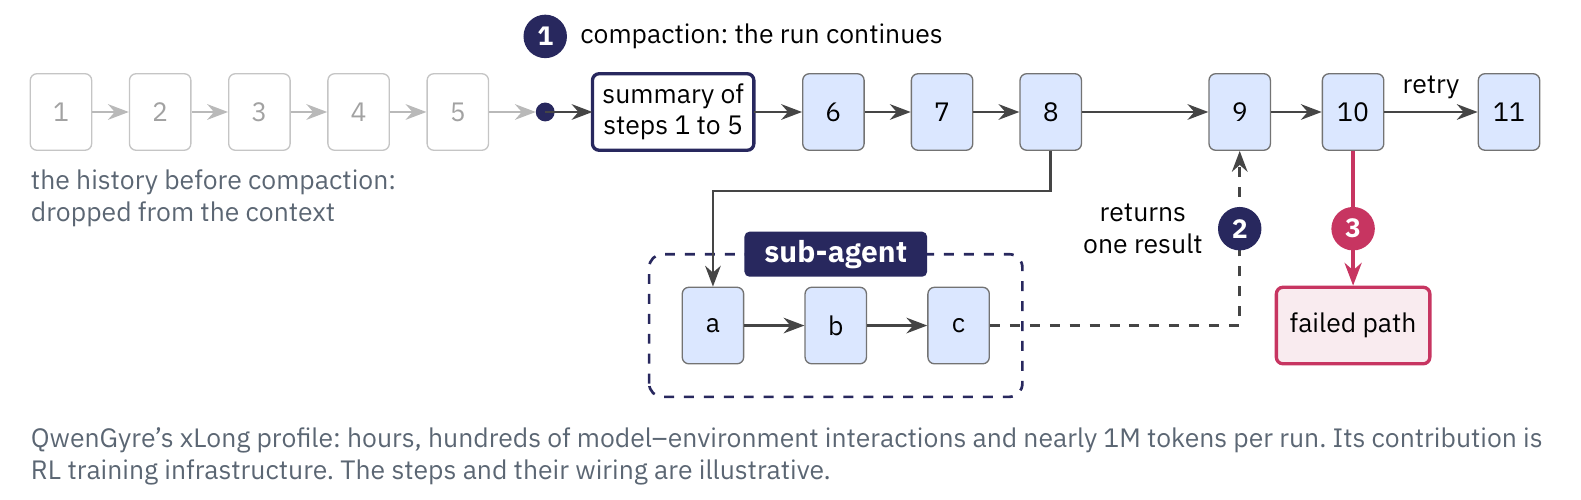
\includegraphics[width=\linewidth]{context/harness-branches-3.png}
\caption{Real harnesses compact, delegate and retry. The figure as it stands after the build's last click.}
\label{fig:harness-branches-3}
\end{figure}

\paragraph{The figure, stage by stage.}
\be
\item Compaction: after step 5 the harness writes the summary of steps 1 to 5, and the run continues from it through step 11. Steps 1 to 5 are the history before compaction, dropped from the context, so no later step sees them.
\item Sub-agent: step 8 hands a subtask to a sub-agent, which runs steps a, b and c in its own context. The sub-agent returns one result to step 9, so the main run never holds steps a, b and c.
\item Failed path: step 10 starts a path that fails, and the harness retries, so the arrow from step 10 to step 11 is the retry. The run is now a graph of context paths, and the note gives QwenGyre's xLong profile: hours, hundreds of model--environment interactions and nearly 1M tokens per run.
\ee

\begin{takeaway}At extreme-long horizons, compaction runs continuously and in layers.\end{takeaway}

\subsection{Pi compacts into a structured summary}
\label{sec:it-7-5a}

\bi
\item \textbf{Summary:} an LLM rewrites the older messages into one summary.
\item \textbf{Recency:} the most recent messages stay, about 20k tokens.
\item \textbf{Structured notes:} fixed sections, from Goal to Critical Context, and file lists.
\ei

Pi 1.2.0's docs/compaction.md describes its compaction. Automatic compaction starts when the tokens in context exceed the context window minus a reserve, 16384 tokens by default, and the user can also enter /compact. Pi keeps the most recent messages, about 20k estimated tokens (keepRecentTokens, a target rather than a cap), summarizes the older ones with an LLM, and rebuilds the context from the system prompt, the summary and the kept messages. The summary has fixed sections: Goal, Constraints \& Preferences, Progress (done, in progress, blocked), Key Decisions, Next Steps and Critical Context. Cumulative lists of the files read and modified follow, and a later compaction includes the previous summary. When the cut falls inside one prompt's span of messages, Pi also summarizes the start of that span under its own headings (Original Request, Progress So Far, Context Needed to Continue) and appends it as a Turn Context section. With earlier messages to summarize as well, that takes a second call.

Pi combines three strategies of the earlier slides: an abstractive summary, recency, and structured notes in its sections and file lists. The defaults are current values that can change.

Pi's documentation describes behaviour and measures nothing.

\begin{figure}[htbp]
\centering
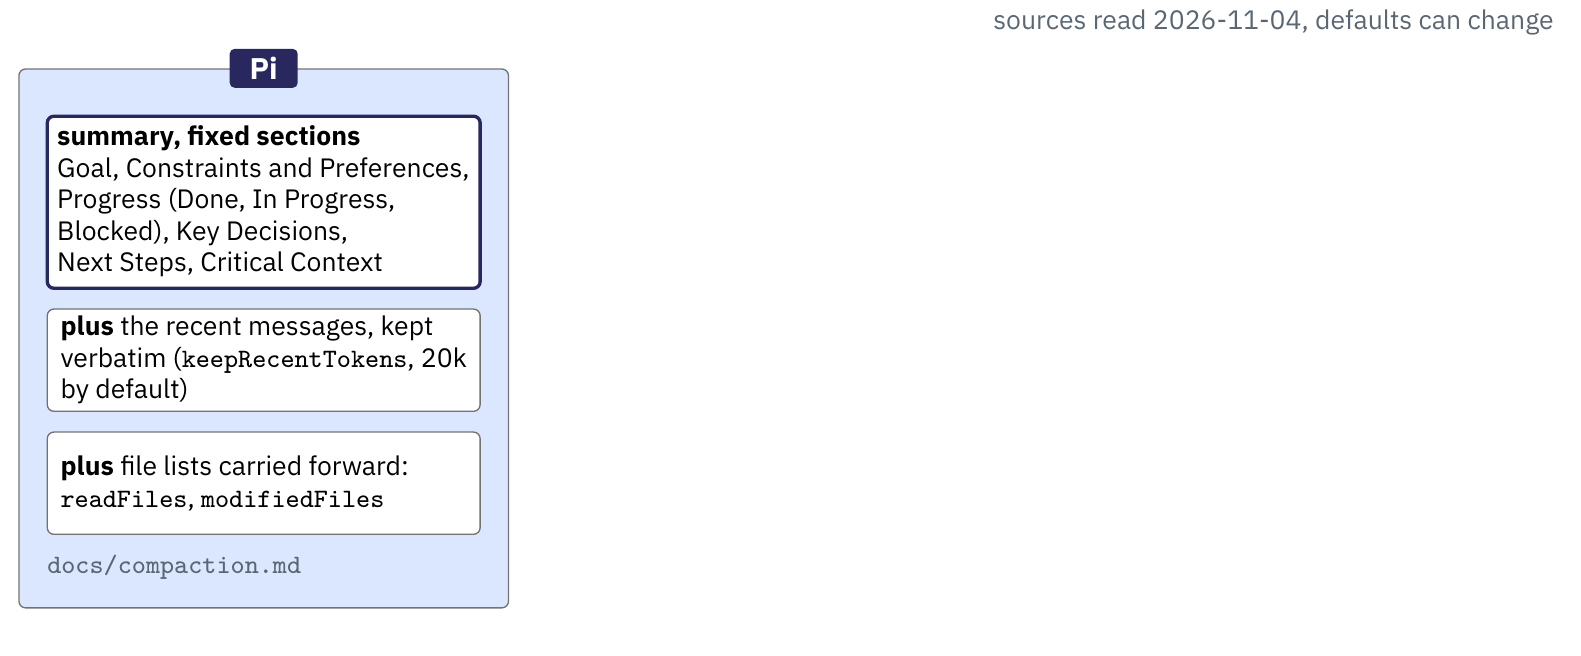
\includegraphics[width=\linewidth]{context/harness-formats-1.png}
\caption{Pi compacts into a structured summary. The figure as it stands after the build's last click.}
\label{fig:harness-formats-1}
\end{figure}

\paragraph{The figure, stage by stage.}
\be
\item The Pi column comes first: a 'summary, fixed sections', from 'Goal' to 'Critical Context', replaces the older messages. Pi also keeps 'the recent messages, kept verbatim (keepRecentTokens, 20k by default)', and its 'file lists carried forward: readFiles, modifiedFiles'.
\ee

\begin{takeaway}Pi pairs a summary with the most recent messages and structured notes.\end{takeaway}

\subsection{Claude Code summarizes and re-reads files}
\label{sec:it-7-5b}

\bi
\item \textbf{Summary:} the conversation becomes a structured summary.
\item \textbf{Retrieval:} it re-reads up to five recently touched files.
\item \textbf{Delegation:} its subagents keep large reads in separate contexts.
\ei

Claude Code's documentation describes its compaction (Explore the context window, \url{https://code.claude.com/docs/en/context-window}, and How Claude Code works, \url{https://code.claude.com/docs/en/how-claude-code-works}, read November 4, 2026). Automatic compaction runs as the window fills, and the user can also enter /compact with a focus. Claude Code replaces the conversation with a structured summary, then reads up to five recently touched files again. A file over 5000 tokens returns as a path reference. SessionStart hooks with the compact source add their output again, the text of skills returns within a limit for each skill, and subagents keep large reads in separate contexts.

Claude Code combines an abstractive summary with retrieval of recent files and with delegation. The thresholds are current values that can change.

Claude Code also compacts at the threshold that /autocompact sets. Its documentation describes behaviour and measures nothing.

\begin{figure}[htbp]
\centering
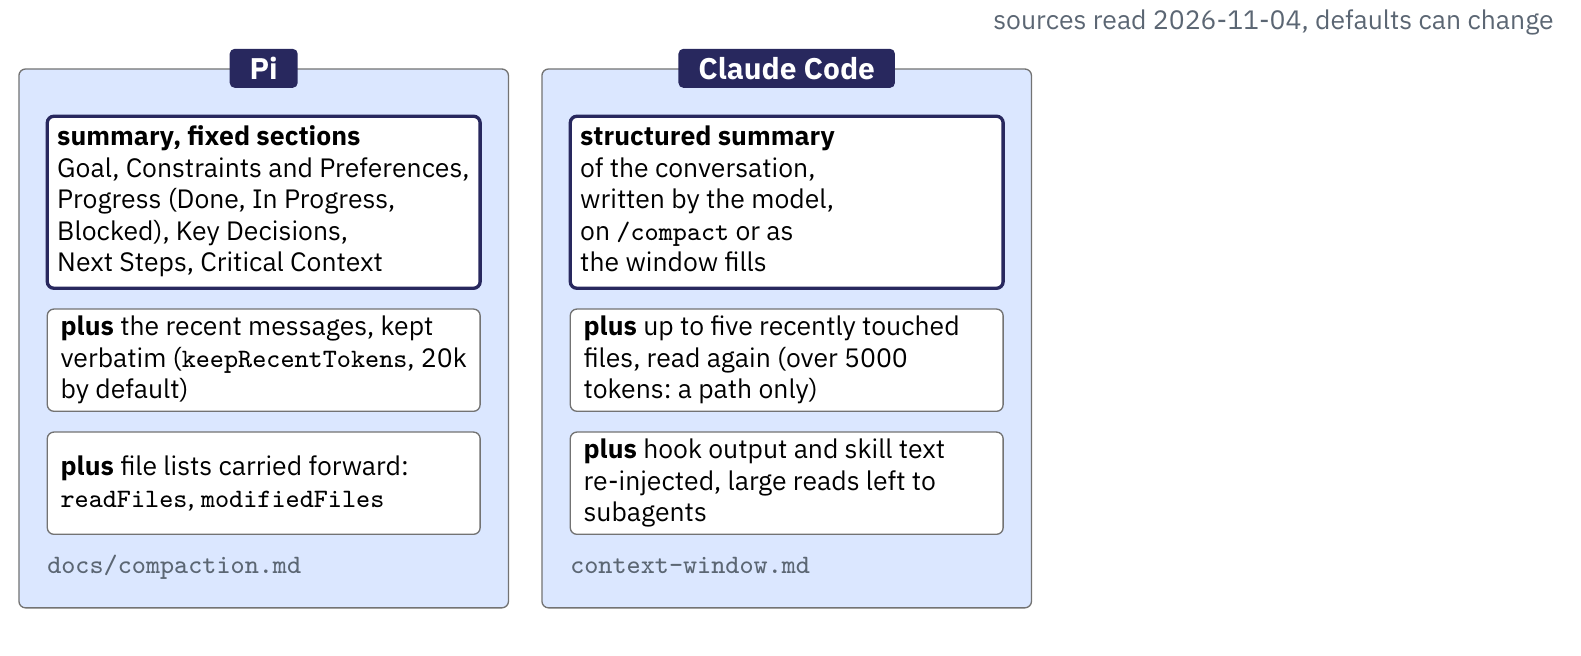
\includegraphics[width=\linewidth]{context/harness-formats-2.png}
\caption{Claude Code summarizes and re-reads files. The figure as it stands after the build's last click.}
\label{fig:harness-formats-2}
\end{figure}

\paragraph{The figure, stage by stage.}
\be
\item The Pi column comes first: a 'summary, fixed sections', from 'Goal' to 'Critical Context', replaces the older messages. Pi also keeps 'the recent messages, kept verbatim (keepRecentTokens, 20k by default)', and its 'file lists carried forward: readFiles, modifiedFiles'.
\item The Claude Code column adds a 'structured summary' of the conversation, 'written by the model, on /compact or as the window fills'. Under it Claude Code reads 'up to five recently touched files' again (a file 'over 5000 tokens' comes back as 'a path only') and re-injects 'hook output and skill text', while 'large reads' are 'left to subagents'.
\ee

\begin{takeaway}Claude Code pairs a summary with a recent-file re-read.\end{takeaway}

\subsection{Codex's local path writes a handoff summary}
\label{sec:it-7-5c}

\bi
\item \textbf{Summary:} a context-checkpoint handoff summary for the next model.
\item \textbf{Retain:} it keeps the user's latest messages beside the summary.
\item \textbf{Structured notes:} an opt-in memories pipeline across sessions.
\ei

The compaction prompt is in the openai/codex repository at commit de6e72a, read November 4, 2026 (codex-rs/prompts/templates/compact/prompt.md and summary\_prefix.md). It calls the step context checkpoint compaction and asks for a handoff summary for another model that will resume the task: progress and key decisions, important context and user preferences, next steps, and critical data or references. Codex rebuilds the history from that summary and the user's most recent messages, up to 20,000 tokens (core/src/compact.rs). It also tells the next model that it still has access to the state of the tools the previous model used, which persists outside the context.

This is the local path. With the default OpenAI provider, Codex uses the remote compaction of the Responses API instead (model-provider/src/capabilities.rs), and the repository shows the summary format only for the local path, which other providers use. Codex compacts automatically when token use reaches its auto-compact limit (model\_auto\_compact\_token\_limit, or the model's default), and the user can also enter /compact. It keeps resume metadata for its sessions, and a memories pipeline, off by default, extracts structured memory across sessions when it is enabled.

Codex combines an abstractive summary with retained user messages and, when enabled, structured notes across sessions.

The memories pipeline runs beside compaction rather than inside it. The repository describes behaviour and measures nothing.

\begin{figure}[htbp]
\centering
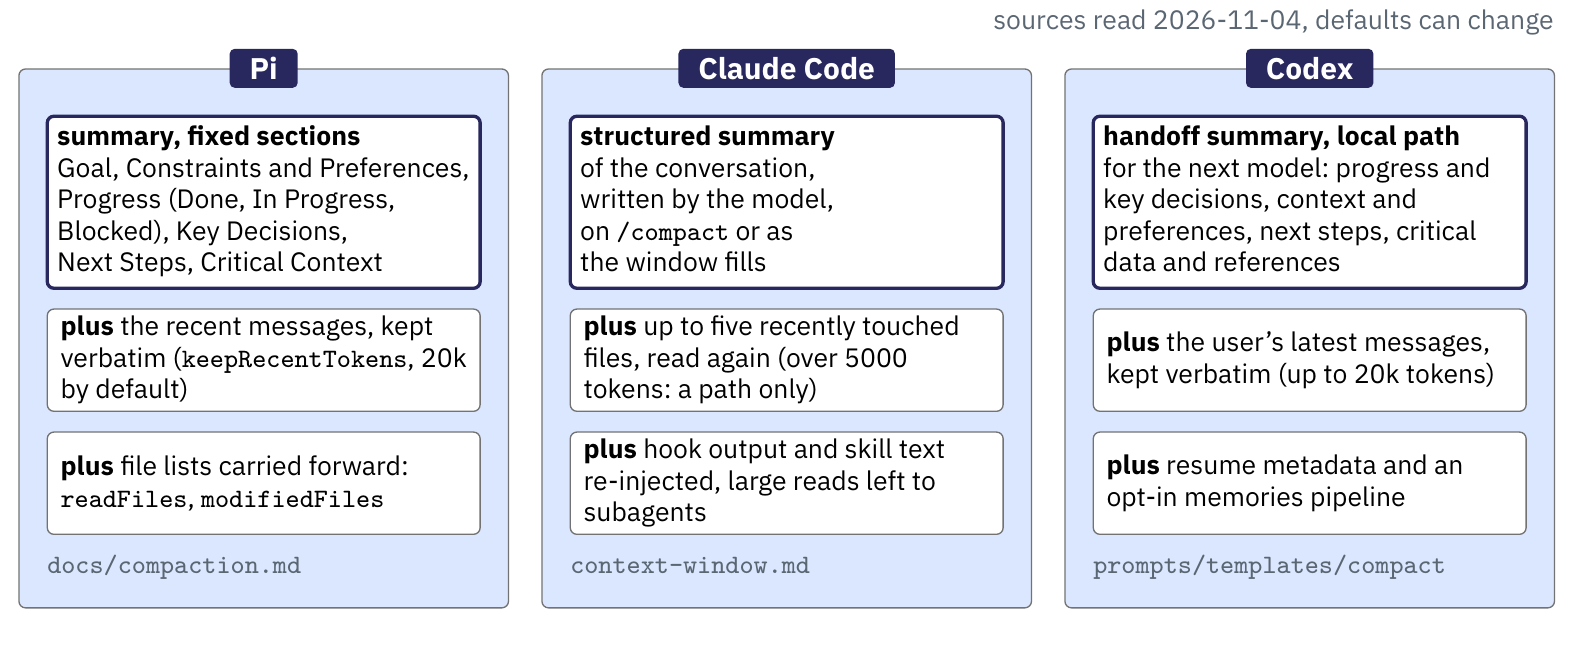
\includegraphics[width=\linewidth]{context/harness-formats-3.png}
\caption{Codex's local path writes a handoff summary. The figure as it stands after the build's last click.}
\label{fig:harness-formats-3}
\end{figure}

\paragraph{The figure, stage by stage.}
\be
\item The Claude Code column adds a 'structured summary' of the conversation, 'written by the model, on /compact or as the window fills'. Under it Claude Code reads 'up to five recently touched files' again (a file 'over 5000 tokens' comes back as 'a path only') and re-injects 'hook output and skill text', while 'large reads' are 'left to subagents'.
\item The Codex column adds a 'handoff summary, local path': when Codex compacts locally, the model writes a summary 'for the next model: progress and key decisions, context and preferences, next steps, critical data and references'. Beside the summary Codex keeps 'the user's latest messages, kept verbatim (up to 20k tokens)', and the third box adds 'resume metadata and an opt-in memories pipeline'.
\ee

\begin{takeaway}Codex pairs a handoff summary with the user's latest messages.\end{takeaway}

\subsection{The harness formats share an abstractive core}
\label{sec:it-7-5d}

The last stage frames the three summaries in navy. All three harnesses build compaction on an abstractive, structured summary, and each adds a second strategy of its own: Pi keeps the most recent messages, Claude Code re-reads recent files, and Codex keeps the user's latest messages. Codex's summary is that of its local path. With the default OpenAI provider, Codex compacts on the server, which returns an encrypted item whose format the repository does not show. The sources are those of the three previous slides.

\begin{figure}[htbp]
\centering
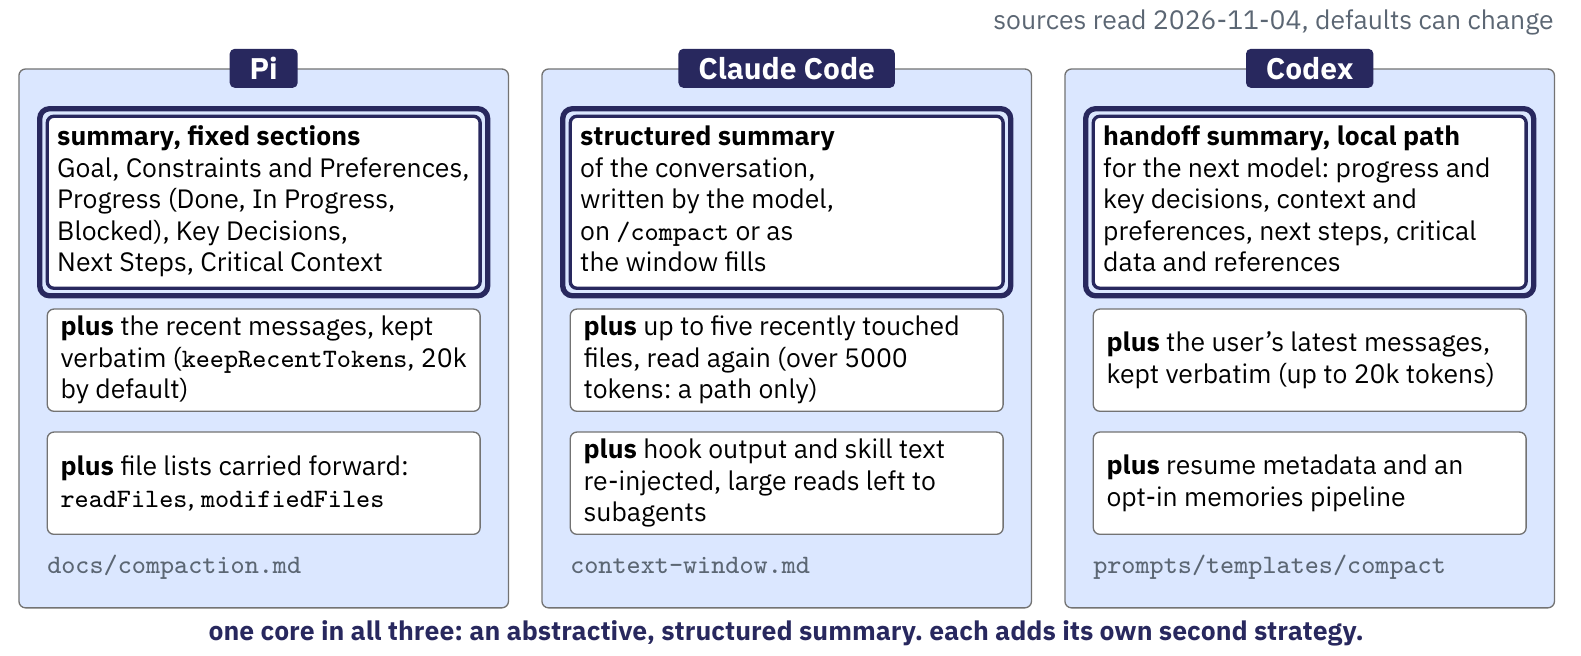
\includegraphics[width=\linewidth]{context/harness-formats-4.png}
\caption{The harness formats share an abstractive core. The figure as it stands after the build's last click.}
\label{fig:harness-formats-4}
\end{figure}

\paragraph{The figure, stage by stage.}
\be
\item The navy frames mark the core all three share, and the caption reads 'one core in all three: an abstractive, structured summary. each adds its own second strategy.' Pi keeps the recent messages, Claude Code reads recent files again, and Codex keeps the user's latest messages.
\ee

\begin{takeaway}Pi, Claude Code and Codex build compaction on an abstractive summary.\end{takeaway}

\subsection{Harness formats compared}
\label{sec:it-7-5e}

\textbf{This table groups the harnesses by the earlier strategies.}

This table recaps the three harness slides, one row per click, in the names of the strategy slides. Pi keeps the most recent messages, Claude Code re-reads recent files and delegates to subagents, and Codex keeps the user's latest messages. Codex's summary format belongs to its local path. With the default OpenAI provider, Codex compacts on the server. The sources are those of the three harness slides, collected in drafts/section-specs/part-02-harness-compaction.md of the lecture folder.

\begin{center}\footnotesize
\begin{tabularx}{\linewidth}{L{0.22\linewidth}XXX}
\toprule
\textbf{Harness} & \textbf{Core} & \textbf{Second strategy} & \textbf{Further strategies} \\
\midrule
Pi & Abstractive structured summary & Recency: recent messages & Structured notes: file lists \\
Claude Code & Abstractive structured summary & Retrieval: recent files & Delegation: subagents \\
Codex & Abstractive handoff summary (local path) & Retain: recent user messages & Structured notes: opt-in memories \\
\bottomrule
\end{tabularx}
\end{center}

\begin{takeaway}Each harness pairs an abstractive summary with other compaction strategies.\end{takeaway}

\subsection{LangGraph can compact one call or the thread}
\label{sec:it-7-6}

\bi
\item \textbf{One call:} \texttt{trim\_messages} or context editing shortens the model's input.
\item \textbf{The thread:} \texttt{SummarizationMiddleware} rewrites the old messages.
\item \textbf{A file:} Deep Agents moves a large tool result out and keeps a preview.
\ei

The coding harnesses compact in their own ways. LangGraph, the framework the course builds agents with, leaves the choice to the developer. It saves an agent's state per thread: the checkpointer writes a checkpoint after every step, so the thread is the agent's short-term memory, and a Store keeps long-term memory across threads. LangChain v1's create\_agent compiles to a LangGraph graph, and its middleware supplies the packaged strategies. We read langchain 1.4.9, langgraph 1.2.20 and deepagents 0.7.32, with their documentation, on November 5, 2026.

For each strategy we ask where its change lands. trim\_messages, from langchain-core, returns a shorter list for one call, and the thread keeps every message. ContextEditingMiddleware with ClearToolUsesEdit also changes one call: it replaces older tool results with ``[cleared]'' in what the model receives, and its source says that it mirrors Anthropic's context editing. SummarizationMiddleware changes the thread: before the model call it writes RemoveMessage(REMOVE\_ALL\_MESSAGES), a summary and the recent messages into the state, and it never separates a tool call from its result. The thread's earlier checkpoints still hold the old messages. Deep Agents, LangChain's agent harness built on LangGraph, moves a tool result of more than 20,000 tokens into a file under /large\_tool\_results/ and keeps a preview of its first and last lines, and its own summarizer keeps the cut history in a file. A developer can also write a @before\_model hook, which changes the thread, or a @wrap\_model\_call hook, which changes one call. The pre\_model\_hook of create\_react\_agent is deprecated.

These map onto the strategies of the earlier slides. Trimming keeps the most recent turns, clearing old tool results masks observations, the summary is abstractive, the file is retrieval by reference, and Deep Agents' subagents delegate.

The numbers in the figure come from a demonstration on the vending run, which the next slide quotes. Its 13 messages hold the Day 1 order in m04 and m05 and the Day 4 request in m13. trim\_messages with max\_tokens=300 returns m10 to m13, so that call never sees the order. SummarizationMiddleware removes m01 to m07, so only the summary carries the order. ClearToolUsesEdit replaces the order confirmation, m05, with ``[cleared]'', while the agent's own message m06 still states the order.

The vending history is scripted, and the message labels, the counts and the tokens come from the capture of the demonstration. The figure leaves out context editing, the Store and subagents, which the notes name. Where the documentation and the code disagree, the research note drafts/section-specs/part-02-langgraph-compaction.md records both.

\begin{figure}[htbp]
\centering
\includegraphics[width=\linewidth]{context/langgraph-compaction-4.png}
\caption{LangGraph can compact one call or the thread. The figure as it stands after the build's last click.}
\label{fig:langgraph-compaction-4}
\end{figure}

\paragraph{The figure, stage by stage.}
\be
\item The thread: LangGraph's checkpointer saves the vending run's thread vm-1, ``13 messages, about 730 tokens'', with ``a checkpoint after every step''. The Day 1 order is m04 and m05, and m13 is the Day 4 request. The grey note names the demonstration, demo.py, run with LangChain 1.4.9.
\item One call: ``trim\_messages: the model receives m10 to m13'', while ``the thread still holds all 13 messages'', so the Day 1 order is ``not in this call'' and comes back on the next one.
\item The thread: ``SummarizationMiddleware: a summary replaces m01 to m07'', and ``the model receives the summary and m08 to m13'', so for ``the Day 1 order'', ``the model sees it only in the summary''. The step-0 checkpoint still holds all 13 messages, which the next slide's capture shows. The one-call box settles to a grey outline.
\item A file: ``Deep Agents: a large tool result moves to a file'', and ``a preview stays, and read\_file reads the rest''. The Day 1 order is ``a short result, so it stays''.
\ee

\begin{takeaway}Each LangGraph compaction changes one call, the thread or a file.\end{takeaway}

\subsection{SummarizationMiddleware rewrites the thread}
\label{sec:it-7-7}

\bi
\item \textbf{The trigger:} past 600 tokens, a summary replaces all but six messages.
\item \textbf{The capture:} the thread loses m01 to m07, and the summary keeps the order.
\ei

The window quotes slides/demos/langgraph/demo.py, lines 161 to 171, and the output quotes four lines of its capture, demo.out.txt, of November 5, 2026, with Python 3.13.15, langchain 1.4.9, langgraph 1.2.20, langchain-core 1.7.6 and langgraph-checkpoint 4.3.1. Both models in the demonstration are fakes (GenericFakeChatModel), so the history, the summary and the agent's reply are scripted. The libraries count the tokens, decide when to summarize, choose the cut, rewrite the state and save the checkpoints.

create\_agent takes the middleware list, and SummarizationMiddleware runs as the node SummarizationMiddleware.before\_model before each model call. trigger=(``tokens'', 600) fires once the thread's messages reach 600 tokens, counted approximately, and keep=(``messages'', 6) keeps the six newest messages as written. A trigger can also count messages or a fraction of the model's input limit, and without one the middleware never runs. By default it keeps 20 messages. The checkpointer, InMemorySaver here, saves the thread at every step.

The capture shows the rewrite. At step 0 the thread holds 13 messages, about 730 tokens. The node writes RemoveMessage(id=''\_\_remove\_all\_\_''), a summary and m08 to m13, so at step 1 the model receives 7 messages. The removed messages, m01 to m07, include the Day 1 order (m04 and m05). The scripted summary keeps the order, its due date and its source: ``Order 17: 10 SKU-A, paid 30.00, due Day 4 (source: inventory-ledger, Day 1)''. A real summarizer writes its own words, and whether they keep the order is the question of the slide \hyperref[sec:it-9-3]{``Each summary leads to a different decision.''} The earlier checkpoints still hold all 13 messages, so the thread's history can recover them, but the agent no longer sees them.

The 600-token trigger suits a short demonstration. Real triggers sit near the model's window: Deep Agents, for example, summarizes at 85 percent of the model's input limit.

\paragraph{demo.py: summarize past 600 tokens, keep the six newest messages}
\begin{footnotesize}
\begin{verbatim}
agent = create_agent(
    model=agent_model,
    middleware=[
        SummarizationMiddleware(
            model=summarizer,          # writes the summary
            trigger=("tokens", 600),   # past 600 tokens in the thread
            keep=("messages", 6),      # the 6 newest stay as written
        ),
    ],
    checkpointer=InMemorySaver(),
)
\end{verbatim}
\end{footnotesize}

\paragraph{output: the checkpoints of thread vm-1, captured November 5, 2026}
\begin{footnotesize}
\begin{verbatim}
step 0  next: SummarizationMiddleware.before_model  13 messages, ~730 tokens
step 1  next: model                                  7 messages, ~502 tokens
the node wrote RemoveMessage(id='__remove_all__'), a summary, m08 to m13
removed from the thread: m01 to m07, the Day 1 order (m04, m05) among them
\end{verbatim}
\end{footnotesize}

\begin{takeaway}A summary that rewrites the thread must carry every open commitment.\end{takeaway}

\subsection*{Key points}
\bi
\item A context policy determines what to keep, fetch, shorten or rewrite.
\item A compressed input is judged by the task it must support.
\item A generated summary becomes another representation that needs checking.
\item Newer compaction is measured, and often trained, on the agent's own tasks.
\item Recency adds no cost, and an open commitment leaves with its old turns.
\item Extraction shortens the text and keeps the original words.
\item A summary restates meaning in new words and needs checking.
\item A running state card carries commitments across every compaction.
\item Delegation moves a subtask's reads out of the main context.
\item Retrieval trades in-context text for a fetch when it is needed.
\item Each strategy buys room by giving up a different kind of recall.
\item At extreme-long horizons, compaction runs continuously and in layers.
\item Pi pairs a summary with the most recent messages and structured notes.
\item Claude Code pairs a summary with a recent-file re-read.
\item Codex pairs a handoff summary with the user's latest messages.
\item Pi, Claude Code and Codex build compaction on an abstractive summary.
\item Each harness pairs an abstractive summary with other compaction strategies.
\item Each LangGraph compaction changes one call, the thread or a file.
\item A summary that rewrites the thread must carry every open commitment.
\ei

\section{What a long horizon demands}
\label{sec:row-2}

Each strategy buys room by giving up a different kind of recall, so the choice depends on what a long run must carry forward. This section takes up the agents lane of the map: METR's measure of how long the tasks agents complete have grown, the state a long run must carry, and Vending-Bench, the benchmark task behind the running example.

\subsection{Time horizons measure tasks in human time}
\label{sec:it-8-0a}

\bi
\item \textbf{The curve:} success falls as tasks take skilled people longer.
\item \textbf{The horizon:} the task length at 50\% success, 4 minutes for GPT-4.
\item \textbf{In 2025:} Claude 3.7 Sonnet reached a horizon of 1 hour.
\item \textbf{In 2026:} Claude Opus 4.6 reached 12 hours, near the suite's 16-hour limit.
\ei

Thomas Kwa, Ben West, Joel Becker and 22 colleagues at METR, Measuring AI Ability to Complete Long Tasks, arXiv:2503.14499, March 18, 2025, published at NeurIPS 2025 as Measuring AI Ability to Complete Long Software Tasks, with the blog post of March 19, 2025 (metr.org/blog/2025-03-19-measuring-ai-ability-to-complete-long-tasks). This is the navy work of the map's agents lane that opens the long-horizon section. It measures what agents can do in a unit people understand: the time a task takes a skilled person. Its 170 tasks run from software actions of a few seconds (SWAA, 66 tasks) through HCAST (97 tasks, from 1 minute to about 30 hours) to RE-Bench's research engineering tasks of 8 hours (7 tasks). Professionals with about five years of experience made more than 800 baseline attempts, 2,529 hours in all, and a task's time is the geometric mean of the successful attempts.

For each model, METR fits a logistic curve of success against the logarithm of a task's human time. The 50\% time horizon is where the curve crosses one half. The 80\% horizon is where it crosses 80 percent, and it is about five times shorter: in the paper, Claude 3.7 Sonnet's horizons were 59 minutes at 50\% and 15 minutes at 80\%. A horizon describes these tasks, mostly well-specified software tasks that a program can score, and says nothing about how long an agent runs.

The figure draws METR's current numbers, Time Horizon 1.1 of January 2026, with 228 tasks and the fit METR corrected on March 3, 2026, as served on November 5, 2026: GPT-4 at 4 minutes, Claude 3.7 Sonnet at 1 hour (60 minutes) and Claude Opus 4.6 at 12 hours (a 95\% interval of about 5 to 61 hours). Each curve is METR's two-parameter logistic, fixed by the model's published 50\% and 80\% horizons. METR writes that the suite ``can't reliably measure time horizons above 16 hours'' (Frontier Risk Report, May 19, 2026), because too few of its tasks are that long, and the grey band marks where the measure runs out.

Every curve is METR's fit on its Time Horizon 1.1 suite, drawn from the model's published 50\% and 80\% horizons, and nothing is illustrative. The three models are three of METR's frontier models, chosen two years apart. The grey band starts at the 16 hours METR names as the suite's limit.

\begin{figure}[htbp]
\centering
\includegraphics[width=\linewidth]{context/metr-curve-4.png}
\caption{Time horizons measure tasks in human time. The figure as it stands after the build's last click.}
\label{fig:metr-curve-4}
\end{figure}

\paragraph{The figure, stage by stage.}
\be
\item The curve: GPT-4's fitted success rate on METR's tasks against the time each task takes a skilled person, on a log scale from 1 second to 32 hours. Success is near 100\% on tasks of seconds and falls toward zero on tasks of hours.
\item The horizon: the dashed line at 50\%, and GPT-4's 50\% time horizon, ringed at 4 min, where its curve crosses one half. That crossing is the definition.
\item 2025: Claude 3.7 Sonnet's curve lies to the right, and it crosses 50\% at 1 h.
\item 2026: Claude Opus 4.6's curve crosses 50\% at 12 h. The grey band past 16 h marks where METR's suite has too few tasks to measure a horizon reliably, and the caption says so.
\ee

\begin{takeaway}A model's time horizon is the human time of the tasks it completes half the time.\end{takeaway}

\subsection{Time horizons grew from seconds to hours}
\label{sec:it-8-0b}

\bi
\item \textbf{The 2025 paper:} horizons doubled about every seven months to 2025.
\item \textbf{The frontier:} Opus 4.6 reached 12 hours, and Opus 5.5 has no METR horizon.
\item \textbf{Since 2023:} on METR's newer suite, the doubling time is about four months.
\item \textbf{The runs:} METR budgets millions of tokens a task and manages the context.
\ei

The blog post's graph is the paper's Figure 1: eleven frontier models from GPT-2 (2019) to Claude 3.7 Sonnet (February 2025), whose 50\% horizons rise from about 2 seconds to 59 minutes. A least-squares line through their logarithms doubles every 212 days, about seven months (95\% interval 171 to 249 days), with R² 0.98. The NeurIPS version adds o3 and reports 207 days. METR printed no table of that figure, so we recomputed it from METR's runs file at commit 2cd6540, which reproduces every horizon the paper prints.

METR has since moved to a larger suite, Time Horizon 1.1 (228 tasks, January 2026), and it stopped updating its dashboard on September 8, 2026. METR says the two suites are not directly comparable, so the figure draws the newer suite throughout, with GPT-2 to GPT-3.5 carried over from the old one as METR's own chart does. On the newer suite, the frontier models since 2023 double about every 129 days, about four months (95\% interval 104 to 158 days), the fit the figure draws. In 2026, Claude Opus 4.6 reached 12 hours (February), Gemini 3.1 Pro 6.4 hours and GPT-5.4 5.7 hours. Claude Mythos Preview (early) measured 17 hours, above the 16 hours the suite can measure, and GPT-5.6 Sol about 11 hours, which METR calls not a robust measurement. For Claude Opus 5.5, METR's report of September 22, 2026 gives no time horizon: it used five other tasks.

The link to context is the run. METR gives its agents budgets of millions of tokens per task: 2 million for its basic scaffold in 2025, 8 to 16 million for the scaffolds of the o-series models, and 16 to 64 million in 2026. Its scaffold ``manages the model's context by organizing its inputs and ensuring they do not exceed the model's maximum context window'' (METR's o3 report, 2025). A task of hours is a run of many calls whose history outgrows one window, the problem of the rest of this section.

Every point is a horizon METR published for a model it marks as the frontier when released, with METR's 95\% interval. The fit is ours, computed as METR describes, and it reproduces METR's 128.7 days. Models that were not the frontier when released, such as Claude Opus 4.1 and Gemini 3.1 Pro, are left out, and the notes give their horizons where they matter.

\begin{figure}[htbp]
\centering
\includegraphics[width=\linewidth]{context/metr-trend-5.png}
\caption{Time horizons grew from seconds to hours. The figure as it stands after the build's last click.}
\label{fig:metr-trend-5}
\end{figure}

\paragraph{The figure, stage by stage.}
\be
\item Seconds: each point is a frontier model's 50\% time horizon on METR's tasks, with its 95\% interval, at its release date, on a log scale from 1 second to 48 hours. GPT-2 (2019), GPT-3 and GPT-3.5 (2022) complete tasks of a few seconds.
\item Minutes: the frontier models of 2023 and 2024, from GPT-4 at 4 minutes to o1 at 39 minutes.
\item Hours: the frontier models of 2025, from Claude 3.7 Sonnet at 1 hour to GPT-5.2 at about 6 hours.
\item 2026: Claude Opus 4.6 at 12 hours, and Claude Mythos Preview, hollow at 17 hours in the grey band past 16 hours, where METR says its suite has too few tasks to measure.
\item The trend: the dashed line fits the frontier models since 2023 that stay under 16 hours, doubling every 129 days, about four months.
\ee

\begin{takeaway}Tasks of many hours make runs that must manage their context.\end{takeaway}

\subsection{Long runs accumulate state to preserve}
\label{sec:it-8-1}

\bi
\item \textbf{Goals and plans} set what the run is for and how it intends to get there.
\item \textbf{Progress and open commitments} record work done and promises pending.
\item \textbf{Grounded evidence} keeps the observations a later decision will rest on.
\item \textbf{Replanning triggers} mark when new observations should change the plan.
\ei

The strategies showed what each one gives up. A long run shows what it must not lose. A long run accumulates state that later calls need: the goals and the plan, the progress so far and the commitments still open, the evidence that later decisions rest on, and the conditions that should trigger a new plan. The vending run the figures have followed is a Vending-Bench task, and its paid order is an open commitment.

The course combines ideas from two sources. Justin Young's Effective harnesses for long-running agents (Anthropic, November 26, 2025) discusses progress records and verification. That article is engineering guidance and measures nothing. LLM-Planner (Chan Hee Song, Jiaman Wu, Clayton Washington, Brian M. Sadler, Wei-Lun Chao and Yu Su, LLM-Planner: Few-Shot Grounded Planning for Embodied Agents with Large Language Models, ICCV 2023) addresses grounded replanning. The slide \hyperref[sec:it-7-5]{``Real harnesses compact, delegate and retry.''} gave QwenGyre's scale: runs of hours, hundreds of interactions and nearly 1M tokens. The previous slides showed that the tasks agents complete keep getting longer, so the state a run must carry grows with them. The next sections test whether the pending commitment of Day 1 survives compaction.

The record, the price and the days in the figure are the course's illustrative teaching case.

\begin{figure}[htbp]
\centering
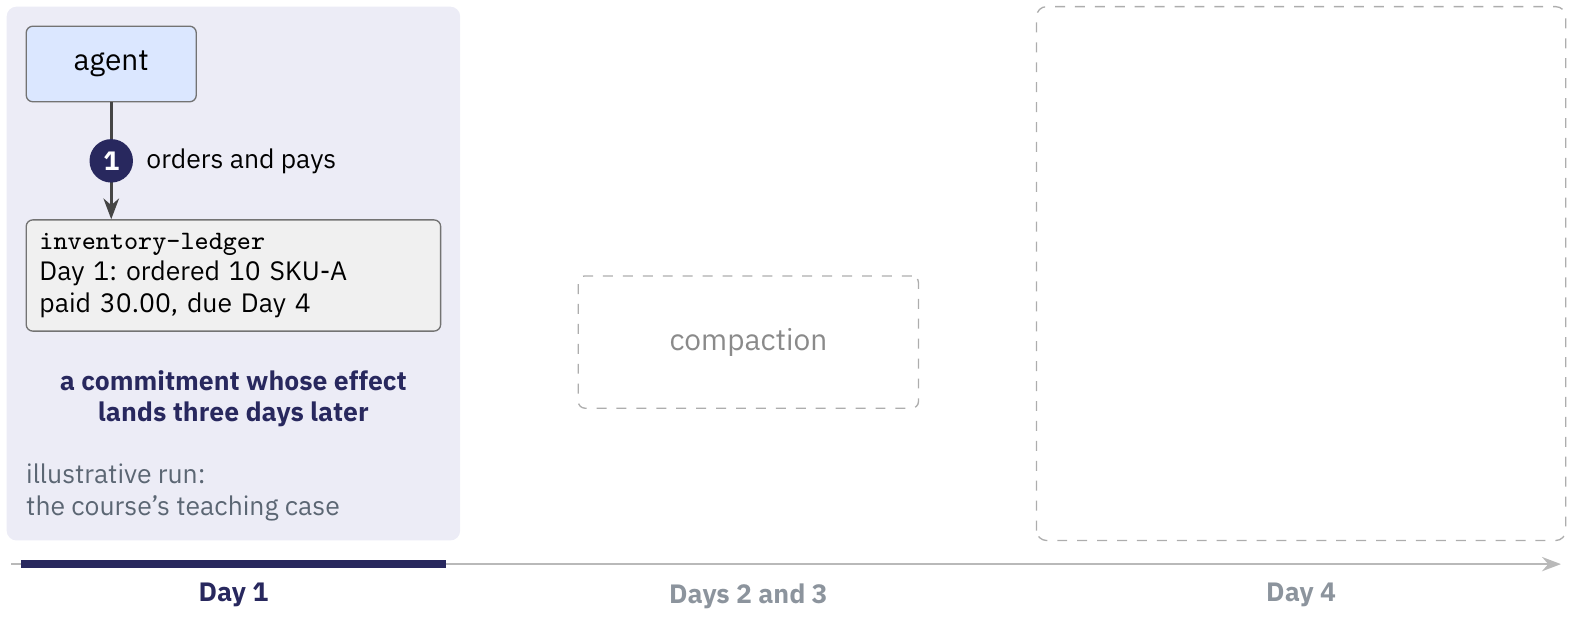
\includegraphics[width=\linewidth]{context/dropped-order-1.png}
\caption{Long runs accumulate state to preserve. The figure as it stands after the build's last click.}
\label{fig:dropped-order-1}
\end{figure}

\paragraph{The figure, stage by stage.}
\be
\item Day 1: the agent ``orders and pays'', and the inventory-ledger records ``Day 1: ordered 10 SKU-A'' and ``paid 30.00, due Day 4'', which the navy caption calls ``a commitment whose effect lands three days later''. The grey note reads ``illustrative run: the course's teaching case'', and dashed ghosts hold the places of compaction and Day 4.
\ee

\begin{takeaway}A long run must carry its open commitments forward to act well.\end{takeaway}

\subsection{Vending-Bench stresses long-term coherence}
\label{sec:it-8-2}

\bi
\item \textbf{The task:} an agent runs a vending business (Andon Labs, preprint, 2025).
\item \textbf{The horizon:} many simulated days, with delayed deliveries and a daily fee.
\item \textbf{The reported failure:} some long runs misread deliveries, full window or not.
\item \textbf{Why it fits:} the run's state outgrows one context and must be carried forward.
\ei

Axel Backlund and Lukas Petersson (Andon Labs), Vending-Bench: A Benchmark for Long-Term Coherence of Autonomous Agents, arXiv:2502.15840, February 20, 2025, a preprint. This is the navy work of the map's agents lane, the task Part II studies in depth, and the vending run the figures have followed is set in it. The agent runs a vending-machine business over simulated calendar time: it checks inventory, orders stock, sets prices and pays a daily fee. Decisions span many simulated days, orders arrive after a delivery delay, and the fee recurs. Over long runs, agents can lose long-term coherence: they misread stock and deliveries, and in some runs they wind the business down early. The run's state outgrows one context, so the agent must preserve information between calls.

Andon Labs released Vending-Bench 2 on November 18, 2025 (andonlabs.com/evals/vending-bench-2, a benchmark page with a leaderboard) and now marks the original as deprecated. Vending-Bench 2 runs a simulated year and adds adversarial suppliers, deliveries that arrive later than promised and suppliers that go out of business. Part II studies the task as the 2025 paper defines it.

Jimenez et al., SWE-bench: Can Language Models Resolve Real-World GitHub Issues?, ICLR 2024 (arXiv:2310.06770v2, April 2024), shows that real GitHub issues are hard for language models: resolving one often needs coordinated edits across several functions and files. With BM25 retrieval and one generated patch per issue, the best of the models in that version, Claude 2, resolved 1.96\% of 2,294 issues, and 4.8\% when given the files the reference patch edited. The paper evaluates no agents, and these rates hold only for the 2023 models and that setup. We keep the simulated calendar duration distinct from the agent's wall-clock runtime and from the depth of its plan. The exact Vending-Bench figures stay in the source paper. Our delayed-delivery case illustrates the paper's type of coherence failure.

The run in the figure is the course's teaching case. In the paper, the agent sees the last 30,000 tokens of its history in most experiments, together with a scratchpad, a key-value store and a vector database, and no summary step. Products arrive a few days after an order, and a daily fee recurs. The authors find no clear correlation between the failures and the point at which the model's context window fills, and their examples include ordering new stock instead of restocking from storage, believing that orders had arrived before they had, and announcing the closure of the business. The compaction step in our figure therefore illustrates the class of failure the paper reports, and we attribute none of the paper's failures to compaction.

\begin{figure}[htbp]
\centering
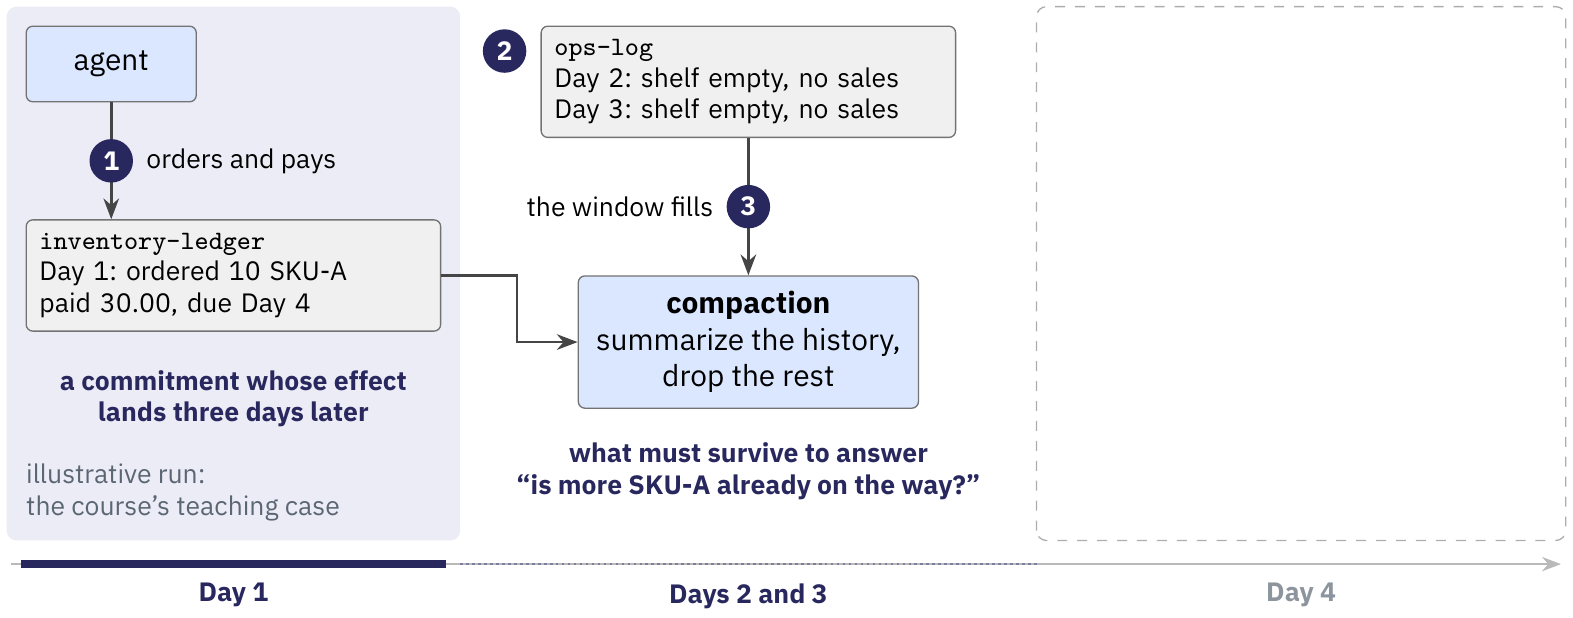
\includegraphics[width=\linewidth]{context/dropped-order-2.png}
\caption{Vending-Bench stresses long-term coherence. The figure as it stands after the build's last click.}
\label{fig:dropped-order-2}
\end{figure}

\paragraph{The figure, stage by stage.}
\be
\item Day 1: the agent ``orders and pays'', and the inventory-ledger records ``Day 1: ordered 10 SKU-A'' and ``paid 30.00, due Day 4'', which the navy caption calls ``a commitment whose effect lands three days later''. The grey note reads ``illustrative run: the course's teaching case'', and dashed ghosts hold the places of compaction and Day 4.
\item The ops-log for Days 2 and 3 records ``Day 2: shelf empty, no sales'' and ``Day 3: shelf empty, no sales'', and when ``the window fills'', compaction reads the ledger and the log to ``summarize the history, drop the rest''. The navy question asks ``what must survive to answer ``is more SKU-A already on the way?''''.
\ee

\begin{takeaway}A long run forces a choice about what to carry forward.\end{takeaway}

\subsection*{Key points}
\bi
\item A model's time horizon is the human time of the tasks it completes half the time.
\item Tasks of many hours make runs that must manage their context.
\item A long run must carry its open commitments forward to act well.
\item A long run forces a choice about what to carry forward.
\ei

\section{Compaction as a design procedure}
\label{sec:row-3}

A long run must carry its open commitments forward and each strategy can lose one, so we turn the strategies into a compaction policy, apply it to the vending run and compare two summaries of the same history.

\subsection{A compaction policy specifies choices}
\label{sec:it-9-1}

\bi
\item \textbf{Specify:} the decisions the context must support, and the trigger.
\item \textbf{Select:} what to keep, what to summarize and what to reference.
\item \textbf{Generate:} a replacement that states facts, open items and sources.
\item \textbf{Check:} the replacement against the task, then assemble the request.
\ei

The course proposes this procedure from the objectives and mechanisms of the earlier sections. A policy specifies which future decisions the context must support and when compaction runs. It selects the material to retain verbatim, to summarize, or to leave available by reference. It generates a replacement that states facts, decisions, conditions, unresolved questions and source references explicitly. It then checks the details the task needs, inspects the resulting request and measures the total work.

Each policy choice must be evaluated, and the slide \hyperref[sec:it-10-1]{``An evaluation measures quality and total work.''} gives the checks. A token threshold can trigger compaction, and so can a task boundary or new information. The figure's trigger fires when the window fills, as in the harnesses of the strategies segment, or when the day changes, a task boundary of the vending run. Next week covers durable storage and recovery.

The four choices are the course's proposal, and no cited source proposes them. The entries are the teaching case's: the ledger line, the log, the price list and the check questions agree with the other figures.

\begin{figure}[htbp]
\centering
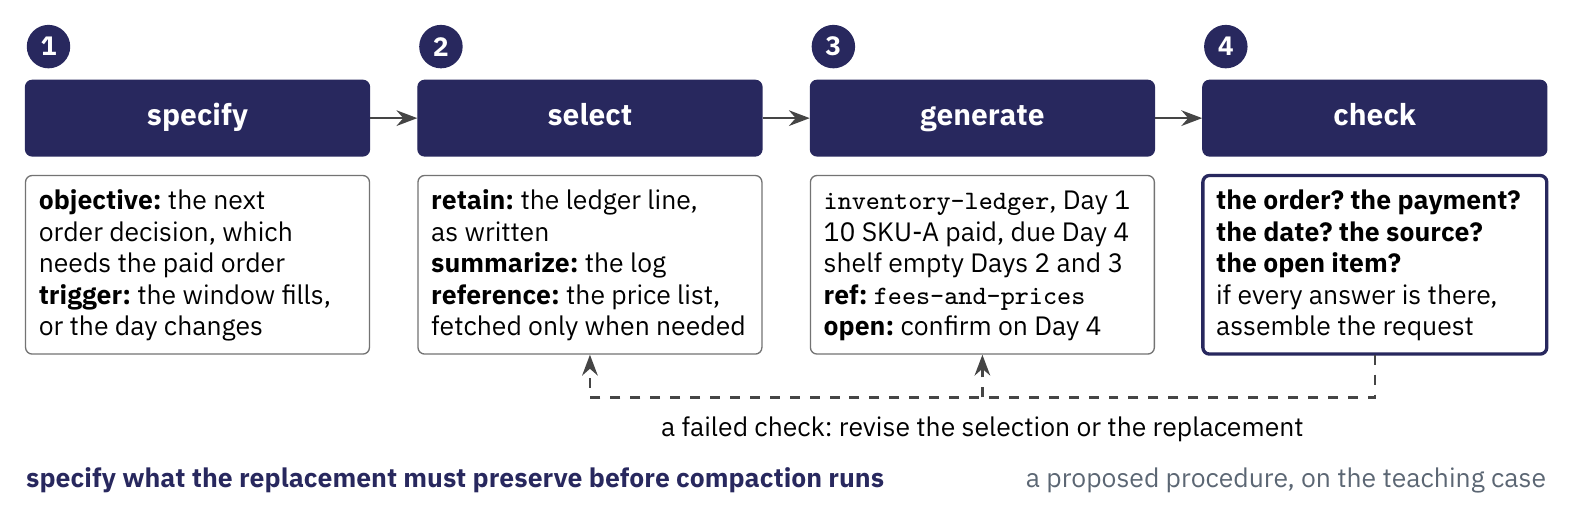
\includegraphics[width=\linewidth]{context/compaction-policy-4.png}
\caption{A compaction policy specifies choices. The figure as it stands after the build's last click.}
\label{fig:compaction-policy-4}
\end{figure}

\paragraph{The figure, stage by stage.}
\be
\item Specify: the objective is ``the next order decision, which needs the paid order'', and the trigger is ``the window fills, or the day changes'': the run compacts when the history reaches the window or when a new day begins. The grey note, ``a proposed procedure, on the teaching case'', marks the procedure as the course's own proposal.
\item Select: ``retain: the ledger line, as written'', ``summarize: the log'' and ``reference: the price list, fetched only when needed''. The ledger line keeps its exact words, the log is reduced to a summary, and the price list stays in its record until a call needs it.
\item Generate: the replacement follows from the selection. It keeps the ledger line as written with its source, ``inventory-ledger, Day 1'' and ``10 SKU-A paid, due Day 4'', summarizes the log as ``shelf empty Days 2 and 3'', points to the price list with ``ref: fees-and-prices'' and states the open item, ``open: confirm on Day 4''.
\item Check: the replacement must answer ``the order? the payment?'', ``the date? the source?'' and ``the open item?'', and the box closes with ``if every answer is there, assemble the request''. The dashed path, ``a failed check: revise the selection or the replacement'', returns to select and generate, and the navy line reads ``specify what the replacement must preserve before compaction runs''.
\ee

\begin{takeaway}A compaction policy decides what survives before any history is replaced.\end{takeaway}

\subsection{Compaction must preserve the pending order}
\label{sec:it-9-2}

\textbf{Two records describe SKU-A on Day 3 of the vending run.}

\bi
\item \textbf{Order record:} \texttt{inventory-ledger}, Day 1: 10 SKU-A paid, due Day 4.
\item \textbf{Shelf record:} \texttt{ops-log}, Days 2 and 3: the SKU-A shelf is empty, no sales.
\ei

We ask which tokens must survive to answer one question: is more SKU-A already on the way? If compaction keeps only the shelf state, the agent sees an empty shelf without the pending order. It can place a second order and pay twice. It can also conclude that the supplier failed and close the business.

This example illustrates the type of coherence failure that Vending-Bench reports. The course supplies these records as a teaching case, and we keep them beside any summary.

The records, the price and the days are illustrative, and the run is the course's teaching case.

The figure is \cref{fig:dropped-order-2} of \cref{sec:it-8-2}.

\paragraph{The figure, stage by stage.}
\be
\item The ops-log for Days 2 and 3 records ``Day 2: shelf empty, no sales'' and ``Day 3: shelf empty, no sales'', and when ``the window fills'', compaction reads the ledger and the log to ``summarize the history, drop the rest''. The navy question asks ``what must survive to answer ``is more SKU-A already on the way?''''.
\ee

\begin{takeaway}A summary must keep the paid order and its due date.\end{takeaway}

\subsection{Each summary leads to a different decision}
\label{sec:it-9-3}

\textbf{Two summaries of the same history reach Day 4.}

\bi
\item \textbf{Summary A} drops the paid order, so the agent orders again and pays twice.
\item \textbf{Summary B} keeps the order, its due date and its source, so the agent waits.
\ei

Both summaries illustrate the teaching case. Summary A reads ``SKU-A is out of stock.'' It loses the paid order and its expected arrival, so the agent places a second order or closes the business. Summary B reads ``SKU-A shelf-empty Days 2 and 3. Ordered 10 units on Day 1 (paid), expected Day 4. Sources: inventory-ledger Day 1 and ops-log Days 2 and 3. Pending: confirm delivery on Day 4.'' The figure shortens it to the order, its source and the check. B keeps the paid order, the expected date and the route to the source.

B is longer because the decision needs the open order. Its references help only while the ledger stays available. A causes the failure of the previous section, and B avoids it.

The two summaries and the second order are the course's illustration.

\begin{figure}[htbp]
\centering
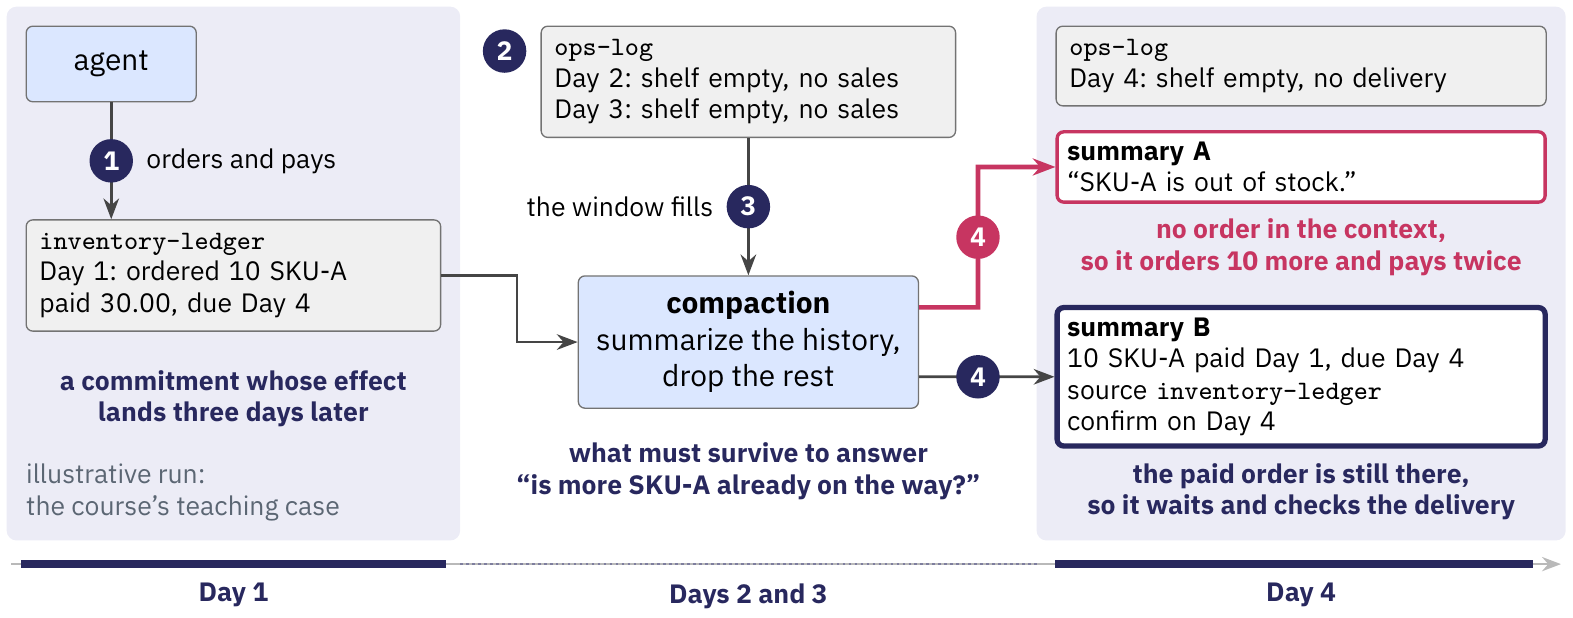
\includegraphics[width=\linewidth]{context/dropped-order-4.png}
\caption{Each summary leads to a different decision. The figure as it stands after the build's last click.}
\label{fig:dropped-order-4}
\end{figure}

\paragraph{The figure, stage by stage.}
\be
\item The ops-log for Days 2 and 3 records ``Day 2: shelf empty, no sales'' and ``Day 3: shelf empty, no sales'', and when ``the window fills'', compaction reads the ledger and the log to ``summarize the history, drop the rest''. The navy question asks ``what must survive to answer ``is more SKU-A already on the way?''''.
\item Summary A reaches Day 4 along the magenta path of event 4 and says only ``SKU-A is out of stock.'' The ledger line is gone from the context, and the new ops-log line ``Day 4: shelf empty, no delivery'' mentions no order, so the magenta verdict reads ``no order in the context, so it orders 10 more and pays twice''.
\item Summary B is the other outcome of the same compaction step, numbered 4 again in navy, and keeps ``10 SKU-A paid Day 1, due Day 4'', ``source inventory-ledger'' and ``confirm on Day 4''. Summary A settles to a magenta outline, and the navy verdict reads ``the paid order is still there, so it waits and checks the delivery''.
\ee

\begin{takeaway}A replacement is judged against the decision it must support.\end{takeaway}

\subsection*{Key points}
\bi
\item A compaction policy decides what survives before any history is replaced.
\item A summary must keep the paid order and its due date.
\item A replacement is judged against the decision it must support.
\ei

\section{Evaluating a context policy}
\label{sec:row-4}

Two summaries of the same history led the agent to different decisions, so we measure a policy by the decisions it supports and by what it costs, stress it with the commitments the run depends on, and close with next week.

\subsection{An evaluation measures quality and total work}
\label{sec:it-10-1}

\bi
\item \textbf{Task success:} the agent makes the right next vending decision.
\item \textbf{Evidence:} the facts, conditions and sources the decision needs survive.
\item \textbf{Faithfulness:} nothing is added or changed, and nothing open is settled.
\item \textbf{Cost:} the token ratio with its convention, and every call, fetch and charge.
\ei

The course combines these measures. Task success checks the next vending decision. Evidence checks the facts, conditions and source references that the decision needs. Faithfulness checks for unsupported claims, changed meaning, and uncertainty that becomes a settled claim. Compression compares the original and replacement token counts under a stated ratio convention. Total work counts summary calls, retrieval, later model calls, elapsed time and charges. The last two share the slide's Cost bullet.

LLMLingua-2 reports task scores, compression and latency together. Include the uncompressed input and a simple selection baseline, compare equal input budgets where possible, and report the uncertainty across repeated runs. A compression ratio alone cannot show that a policy serves its task. These five measures cover the three objectives of the slide \hyperref[sec:it-5-1]{``Context supplies each call within a budget.''} and its cost.

The rubric is the course's, and no paper reports results for it. The ``60k to 40 tokens'' of the compression check reuses the abstractive figure's illustrative counts, so we state the ratio convention with it, for example original over replacement, 1500 to 1.

\begin{figure}[htbp]
\centering
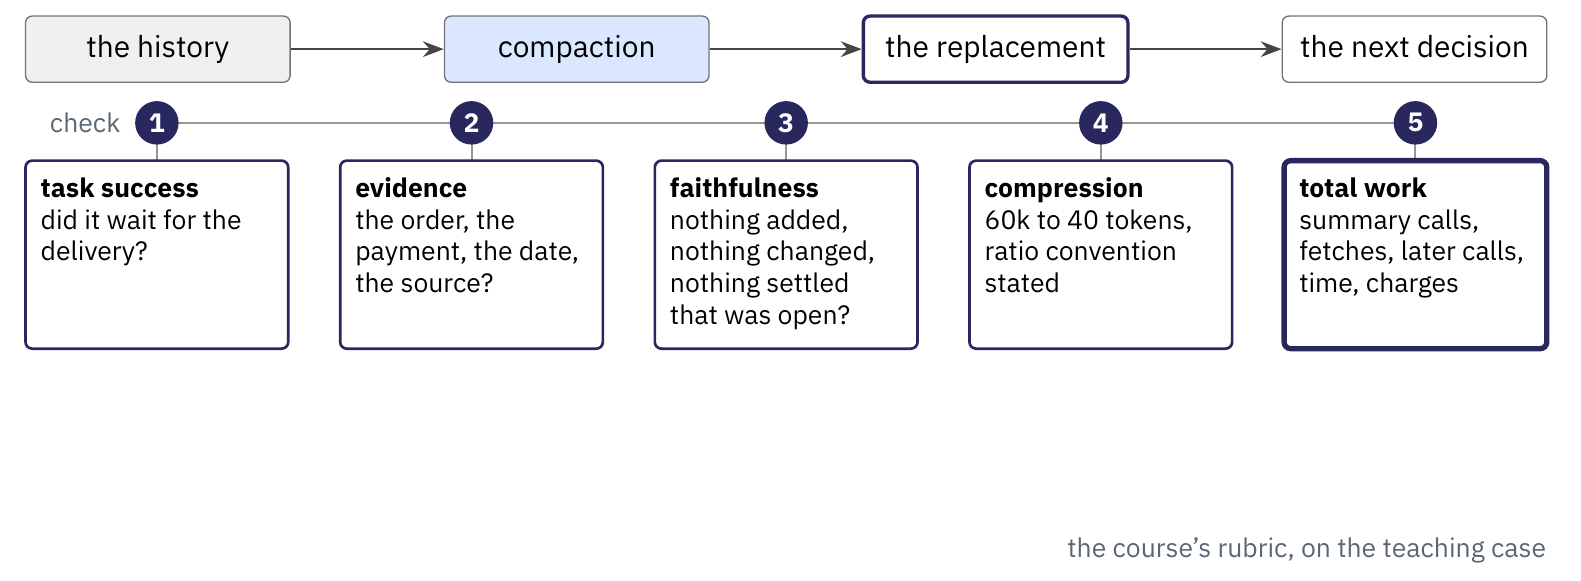
\includegraphics[width=\linewidth]{context/evaluation-5.png}
\caption{An evaluation measures quality and total work. The figure as it stands after the build's last click.}
\label{fig:evaluation-5}
\end{figure}

\paragraph{The figure, stage by stage.}
\be
\item The run lane: compaction turns the history into the replacement, and the next decision is made from the replacement. Check 1, task success, asks of the vending run: did it wait for the delivery?
\item Check 2, evidence: the order, the payment, the date, the source? The replacement must still carry each fact the next decision needs.
\item Check 3, faithfulness: nothing added, nothing changed, nothing settled that was open? Whether the delivery has arrived is still open, and the replacement must keep it open.
\item Check 4, compression: 60k to 40 tokens, ratio convention stated. The counts are those of the abstractive summary that leaves out the paid order, and the report states which way the ratio runs.
\item Check 5, total work: summary calls, fetches, later calls, time, charges. The five checks are reported together, because a compression ratio alone cannot show that a policy serves its task.
\ee

\begin{takeaway}A policy is judged by the decisions it supports and by the work it costs.\end{takeaway}

\subsection{Stress tests target what compaction can lose}
\label{sec:it-10-2}

\bi
\item \textbf{Delayed effects:} a delivery due after the next compaction must stay recorded.
\item \textbf{Recurring obligations:} the daily fee must survive repeated compaction.
\item \textbf{Updates and provenance:} a revised delivery date must carry its source.
\item \textbf{Repeated compaction:} the open order must survive several replacements.
\ei

Each stress test reuses the test logic of RULER and of Lost in the Middle. RULER plants facts with known answers in synthetic text, fixes the task, changes only the input length, scores every answer automatically and grades each length against a fixed bar. Lost in the Middle moves the evidence to chosen positions. A stress test plants a commitment in the run's history, compacts, and checks automatically that the next decision still has it. We vary what the two papers vary: the commitment sits early, in the middle or late in the history, and the history grows to each length the run reaches before it compacts. Two of the drawn tests exercise operations that RULER grades separately (the backup slide \hyperref[sec:it-B-6-3]{``Effective length depends on the operation.''}): the daily fee is one fact to find, and a revised delivery date is a chain to trace to its source. None of the four aggregates, and a full suite adds one, such as the units still on order. The course proposes these application tests, and neither paper reports results for them. The fourth test has published evidence behind it: Agentic Context Engineering (Zhang et al., ICLR 2026) describes context collapse, in which iterative rewriting erodes details over time.

For the vending run, we test an empty shelf while an order remains in transit, a second order before the first arrives, and a delivery notice that changes the expected date. Source access is verified separately from the summary's wording.

The four drawn tests are the course's. Neither the figure nor the bullets show a position or a length test.

\begin{figure}[htbp]
\centering
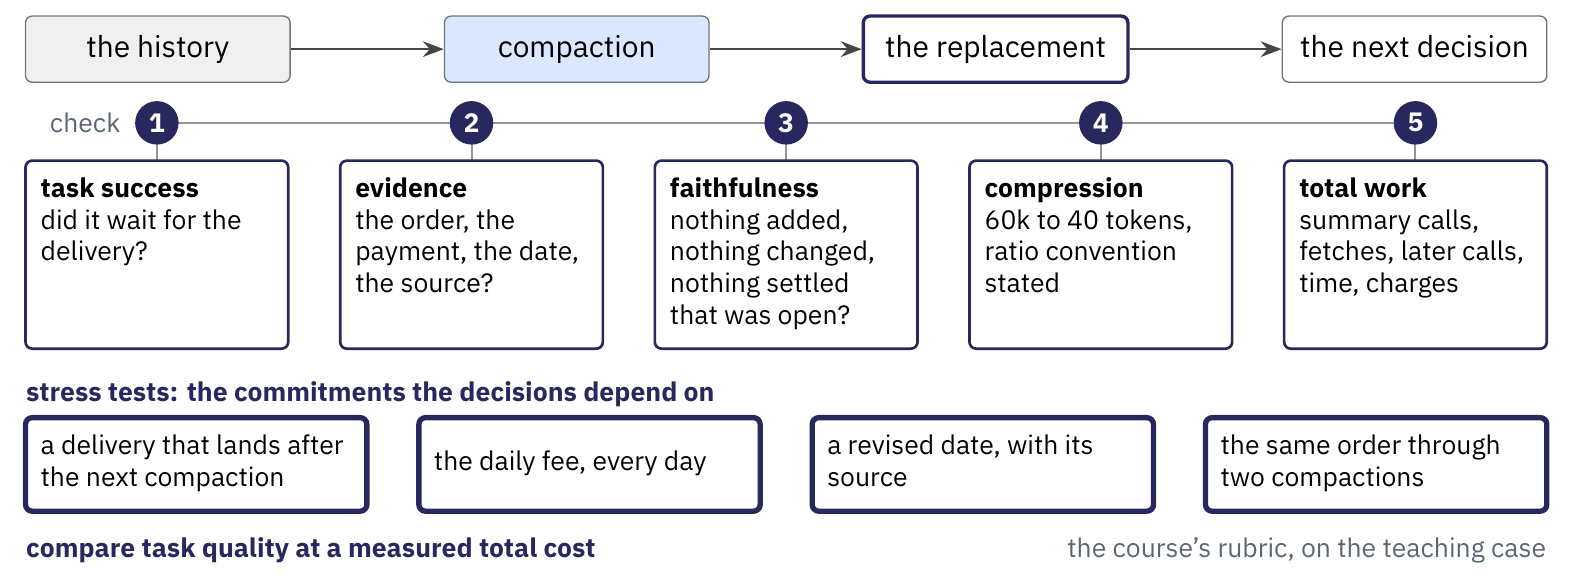
\includegraphics[width=\linewidth]{context/evaluation-6.png}
\caption{Stress tests target what compaction can lose. The figure as it stands after the build's last click.}
\label{fig:evaluation-6}
\end{figure}

\paragraph{The figure, stage by stage.}
\be
\item Check 5, total work: summary calls, fetches, later calls, time, charges. The five checks are reported together, because a compression ratio alone cannot show that a policy serves its task.
\item The stress tests plant the commitments the decisions depend on: 'a delivery that lands after the next compaction', 'the daily fee, every day', 'a revised date, with its source' and 'the same order through two compactions'. The navy line states the rule of the five checks: compare task quality at a measured total cost.
\ee

\begin{takeaway}Each test plants a commitment and checks that it survives compaction.\end{takeaway}

\subsection{Contexts become part of execution state}
\label{sec:it-11-1}

\bi
\item \textbf{Today:} choosing, transforming and evaluating what each call receives.
\item \textbf{Next week:} execution state keeps these contexts for checkpoints, resumption and replay.
\ei

Today we chose, transformed and evaluated what each call receives. Next week keeps these contexts in state: state ownership, run-local and durable state, checkpoint boundaries, resumption and replay. The vending run returns there, because the commitments it carries forward are what a checkpoint must hold.

The lane of steps and checkpoints is schematic, a preview of next week with illustrative counts.

\begin{figure}[htbp]
\centering
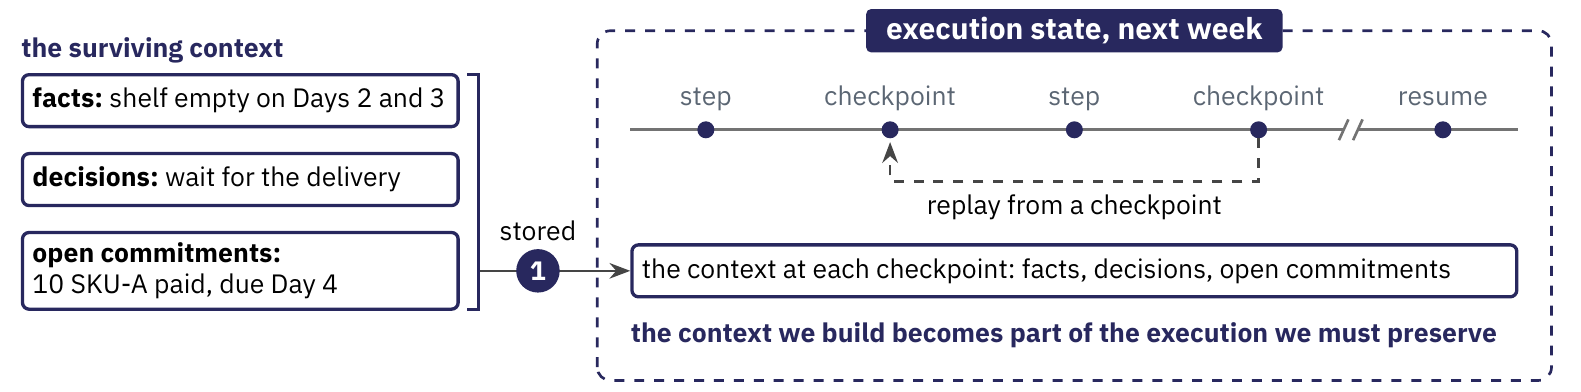
\includegraphics[width=\linewidth]{context/state-bridge-2.png}
\caption{Contexts become part of execution state. The figure as it stands after the build's last click.}
\label{fig:state-bridge-2}
\end{figure}

\paragraph{The figure, stage by stage.}
\be
\item The surviving context: three chips hold ``facts: shelf empty on Days 2 and 3'', ``decisions: wait for the delivery'' and ``open commitments: 10 SKU-A paid, due Day 4''. The dashed ghost ``execution state, next week'' reserves the place where this context goes next.
\item The execution state: the run passes ``step'' and ``checkpoint'' twice, breaks, and goes on at ``resume'', and the dashed arrow marks ``replay from a checkpoint''. A bracket gathers all three chips, and arrow 1, ``stored'', carries them into ``the context at each checkpoint: facts, decisions, open commitments'', so ``the context we build becomes part of the execution we must preserve''.
\ee

\begin{takeaway}A checkpoint must hold the context that the harness has built.\end{takeaway}

\subsection*{Key points}
\bi
\item A policy is judged by the decisions it supports and by the work it costs.
\item Each test plants a commitment and checks that it survives compaction.
\item A checkpoint must hold the context that the harness has built.
\ei

\section{Backup: how much of its window a model can use}
\label{sec:backup}

These builds sit after the last slide of the deck, out of the main sequence. The lecture shows them only when a student asks how much of its window a model can use.

\subsection{Effective length falls short of the window}
\label{sec:it-B-6-2}

\bi
\item \textbf{RULER} (Hsieh et al., 2024) asks how much of its window a model can use.
\item \textbf{The method:} synthetic tasks with more needles, tracing and aggregation.
\item \textbf{The effective length:} the longest tested length above Llama2-7B's 4K score.
\item \textbf{The reported result:} almost every model's effective length is below its claim.
\ei

Cheng-Ping Hsieh, Simeng Sun, Samuel Kriman, Shantanu Acharya, Dima Rekesh, Fei Jia, Yang Zhang and Boris Ginsburg (NVIDIA), RULER: What's the Real Context Size of Your Long-Context Language Models?, First Conference on Language Modeling (COLM 2024). We use arXiv:2404.06654 version 3 of August 6, 2024, the COLM version, which evaluates 17 models and keeps version 1's numbers for GPT-4, Yi (34B) and LWM (7B). The OpenReview record lists seven authors, without Yang Zhang. RULER is the companion to Lost in the Middle, and one of its needle tasks is that paper's key-value retrieval. On the map it sits in the evaluations lane.

The paper asks how much of its claimed window a model can use. Model releases of 2024, among them Gemini 1.5 and Claude 3, reported their long windows with the needle-in-a-haystack test, which Section 1 names beside passkey retrieval as the common synthetic tests. That test hides one fact, the needle, in long filler text, the haystack, and asks for it. The abstract calls it ``indicative of only a superficial form of long-context understanding''. GPT-4, Yi (34B) and LWM (7B) score 100.0 on it and on passkey retrieval at every length from 4K to 128K (Tables 10 and 11), so by these tests every window looks usable.

RULER keeps the needle test's control, synthetic text of a chosen length with a known answer, and makes the tasks harder. Its 13 tasks fall into four categories (Section 3). Retrieval keeps the single needle, with the passkey and vanilla needle tests among its eight tasks, and adds the needle among distractor needles and requests for several values or several keys. Multi-hop tracing follows a chain of variable bindings, X2 = X1, X3 = X2 and on, and returns every name bound to one value. Aggregation returns the most frequent words of a long list. Question answering hides the paragraphs that answer a SQuAD or HotpotQA question among other paragraphs. Each task runs at 4K, 8K, 16K, 32K, 64K and 128K tokens, and the score at a length is the mean accuracy over the 13 tasks (Section 4).

The effective length turns each curve into one number. The bar is 85.6, the 13-task mean of Llama2-7B (chat), a model with a 4K window, at 4K. The longest tested length whose mean exceeds the bar is the model's effective length, which Table 3 prints beside its claimed length (Section 4, ``Effective Context Size''). A long-context model therefore counts as effective at a length while it still beats a 7B model working at 4K. Table 3 grades only these six lengths, so it never grades a claim above 128K at the claim itself.

Every model in Table 3 except Gemini-1.5-Pro falls below the bar before its claimed length. Gemini-1.5-Pro stays above the bar at every tested length, 94.4 at 128K, and its 1M claim was not tested. Ten of the 17 models pass the bar at 32K, which the abstract reports as ``only half of them''. An et al. (Why Does the Effective Context Length of LLMs Fall Short?, ICLR 2025) trace the gap to training: relative positions far apart are rarely trained, and open models' effective lengths typically stay under half their training lengths. The next slide shows that the effective length also depends on the operation.

Every value in the chart is printed in version 3 of the paper: the needle scores in Table 11 (p. 24), and the 13-task means, the bar and the claimed and effective lengths in Table 3 (p. 7). None is read off a figure. The three models are three of the four that score 100.0 on the vanilla needle test at every length. The fourth, GLM4 (9B), is left out because its line would run beside GPT-4's. The lines join the six lengths of Tables 3 and 11, the only lengths they measure, and the accuracy axis starts at 60. RULER places the evidence at varied depths but reports one number per length, with no accuracy by position, the variable Lost in the Middle studies. The paper lists this first among its limitations (Section 8, ``Lack of position controlling''). In the second, the authors offer RULER as ``convenient behavioral checks'' that ``should not be preferred over more realistic settings''. The results describe models evaluated in 2024 on synthetic tasks, and a present model needs its own measurement.

\begin{figure}[htbp]
\centering
\includegraphics[width=\linewidth]{context/effective-length-5.png}
\caption{Effective length falls short of the window. The figure as it stands after the build's last click.}
\label{fig:effective-length-5}
\end{figure}

\paragraph{The figure, stage by stage.}
\be
\item The key lists three models evaluated in 2024 and the windows their makers claim: 128K tokens for GPT-4, 200K for Yi (34B) and 1M for LWM (7B). On the vanilla needle test, which hides one fact in filler text, all three score 100.0 at every length from 4K to 128K, the longest length of the paper's main tables (Tables 3, 10 and 11). By this test every window looks usable, and RULER asks how much of it each model can use.
\item The blue line is GPT-4 on RULER: the mean accuracy over 13 synthetic tasks with more needles, tracing and aggregation, the passkey and needle tests among them. Those two stay at 100.0, so the fall from 96.6 at 4K to 81.2 at 128K comes from the other eleven tasks. Strong simple retrieval coexists with a falling score on harder tasks.
\item The dashed bar is 85.6, the mean that Llama2-7B, a 7B model with a 4K window, scores at 4K. A model's effective length is the longest tested length whose mean exceeds the bar. GPT-4 scores 87.0 at 64K and 81.2 at 128K, so its effective length is 64K, half its claimed 128K. The ring marks that point.
\item Yi (34B) falls from 93.3 at 4K to 77.3 at 128K. Its last length above the bar is 32K, at 87.5, against a claimed 200K, beyond the six lengths of Table 3. Section 5 of the paper tests this model on single tasks up to 256K, its claim included, and analyzes its errors.
\item LWM (7B) starts at 82.3, already below the bar at 4K, and ends at 65.0. Table 3 prints its effective length as under 4K against a claimed 1M, although it scores 100.0 on the needle test at every length. The bullet that arrives with it states the result for all 17 models: almost every effective length is below the claim.
\ee

\begin{takeaway}The needle test overstates how much of a window a model can use.\end{takeaway}

\subsection{Effective length depends on the operation}
\label{sec:it-B-6-3}

\bi
\item \textbf{In the vending run,} a decision needs one fact, a chain of facts or a total.
\item \textbf{In RULER,} Llama3.1 (8B) is effective to 64K at finding, 8K at aggregating.
\item \textbf{In a harness,} each call should stay within its operations' effective lengths.
\ei

Hsieh et al., RULER, COLM 2024, as on the slide \hyperref[sec:it-B-6-2]{``Effective length falls short of the window.''} The figure adapts three of RULER's task categories to the vending log. Finding one fact is retrieval, following a chain of facts is multi-hop tracing, and combining many lines is aggregation. The decisions of the vending run need all three: the daily fee is one line, the due date of order 17 follows through shipment 5, and the units on order add up across five lines.

RULER also grades each category on its own, against Llama2-7B's 4K score on that category: 96.9 for retrieval, 89.7 for tracing and 84.8 for aggregation (Appendix F, Tables 13 to 15). On the 13-task mean, Llama3.1 (8B) is effective to 32K. By category, it is effective to 64K on retrieval and on tracing, and to 8K on aggregation, where its accuracy falls from 97.0 at 4K to 54.1 at 32K (Table 15). GLM4 (9B) and GradientAI/Llama3 (70B) also reach only 8K on aggregation. The order differs by model: GPT-4 is effective to 32K on retrieval, 128K on tracing and 64K on aggregation. One effective length per model therefore overstates the usable length for some operations and understates it for others.

The third bullet is the course's reasoning, and RULER evaluates no harness. The harnesses of the strategies segment compact as the window fills: Pi when the tokens in context exceed the window minus a reserve, 16384 tokens by default, and Claude Code as the window fills (the slides \hyperref[sec:it-7-5a]{``Pi compacts into a structured summary.''} and \hyperref[sec:it-7-5b]{``Claude Code summarizes and re-reads files.''}). A context that grows to the window can pass the length at which the operations a decision needs still work. Compaction helps in two ways. It keeps each call short, and a summary that records the resolved chain (order 17, due Day 4) or the running total (26 units ordered in all) turns a later trace or aggregate over a long log into a find over a short one. The summary step is itself an aggregation over the history, the category RULER offers as its proxy for summarization (Section 3.3), and aggregation fails first for Llama3.1 (8B), so the summarizer also needs an input it can use. RULER's numbers describe models evaluated in 2024 on synthetic tasks, so a run measures these lengths on its own model and operations.

The slide \hyperref[sec:it-10-2]{``Stress tests target what compaction can lose.''} reuses this test logic. It plants a commitment with a known answer in the run's history, compacts, and checks automatically that the next decision still has it.

The log lines, the highlighted lines and the three answers are illustrative. The rows adapt three of RULER's categories to a vending log: find stands for retrieval, trace for variable tracking, and aggregate for common-word and frequent-word extraction. Those two tasks count words, where the figure adds units. The figure draws no length and claims no score. RULER's fourth category, question answering, is left out. Its bar is 49.7, so its effective lengths come out long although its scores start lowest: at 4K, question answering is the lowest of the four categories for 16 of the 17 models (Tables 13 to 16). RULER generates its own synthetic inputs for each task at each length. The effective lengths of the second bullet are those of Tables 13 and 15, for a model evaluated in 2024.

\begin{figure}[htbp]
\centering
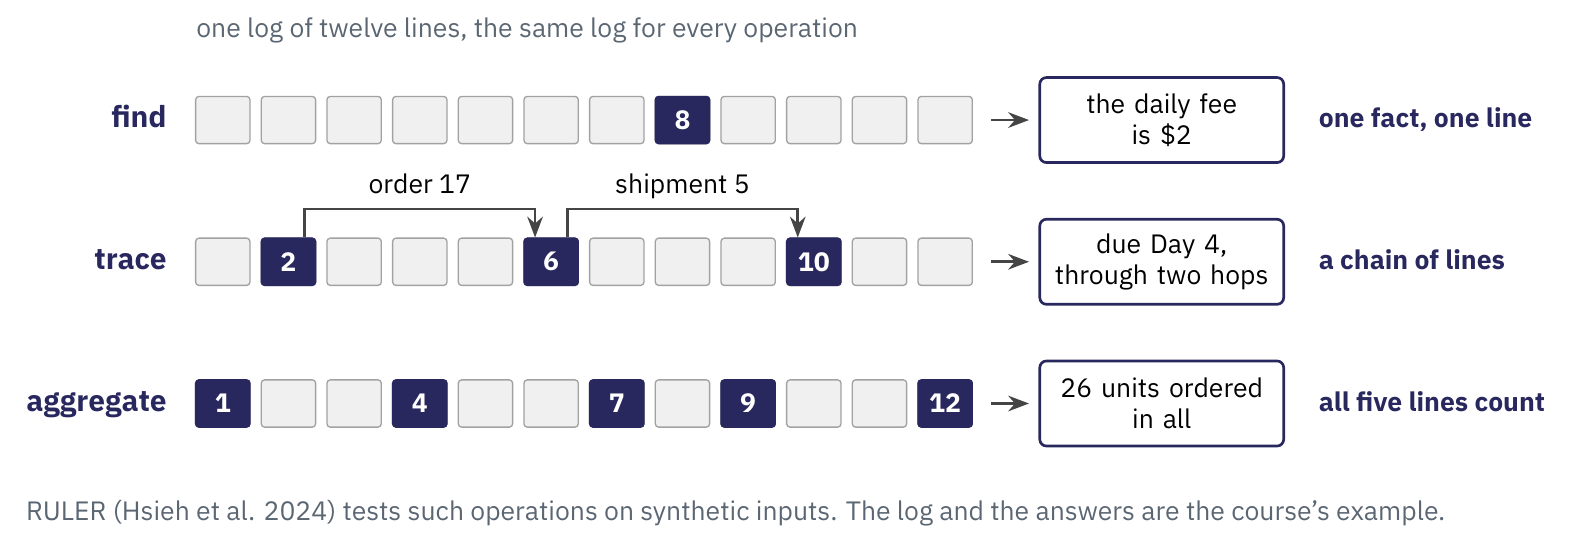
\includegraphics[width=\linewidth]{context/context-tasks-3.png}
\caption{Effective length depends on the operation. The figure as it stands after the build's last click.}
\label{fig:context-tasks-3}
\end{figure}

\paragraph{The figure, stage by stage.}
\be
\item Find: line 8 alone holds the answer, the daily fee is \$2, so the verdict reads one fact, one line. This is RULER's retrieval, the needle test and its harder variants, on the run's own log. Every later row reads the same log of twelve lines.
\item Trace: line 2 points to line 6 through order 17, and line 6 points to line 10 through shipment 5. The answer, due Day 4, through two hops, needs a chain of lines. RULER's variable tracking follows a chain of bindings in the same way: X2 = X1, X3 = X2 and on.
\item Aggregate: the answer, 26 units ordered in all, adds up lines 1, 4, 7, 9 and 12. All five lines count, so a model that misses any one of them returns a wrong total. The bullet that arrives with this row gives RULER's measurement for Llama3.1 (8B): effective to 64K at finding and to 8K at aggregating.
\ee

\begin{takeaway}A harness must test the operations its task needs at the lengths it expects.\end{takeaway}

\section{Reading list}
\label{sec:reading}

The reading list maps the research the lecture draws on, in the seven groups of the deck's backup tables. Rows run by first public release, and the full references follow each table.

\subsection{Reading on long-context evaluation}
\label{sec:it-R-eval}

\begin{center}\footnotesize
\begin{tabularx}{\linewidth}{L{0.26\linewidth}L{0.2\linewidth}X}
\toprule
\textbf{Work} & \textbf{Venue} & \textbf{Contribution} \\
\midrule
Shi et al. & ICML 2023 & Irrelevant sentences cut math accuracy \\
Passkey retrieval & NeurIPS 2023 & A passkey hidden in long filler text \\
Lost in the Middle & TACL 2024 & Accuracy is often lowest with mid-input evidence \\
LongBench & ACL 2024 & 21 datasets in six task types, English and Chinese \\
Needle In A Haystack & GitHub, 2023 & One fact hidden at set depths in filler \\
Same Task, More Tokens & ACL 2024 & Accuracy falls on inputs padded to 3,000 tokens \\
RULER & COLM 2024 & Effective length below the claimed length \\
HELMET & ICLR 2025 & Needle scores predict application scores poorly \\
An et al. & ICLR 2025 & Rarely trained positions shorten effective length \\
NoLiMa & ICML 2025 & Scores fall without literal overlap \\
Context Rot & Chroma report, 2025 & Accuracy falls unevenly as input grows \\
\bottomrule
\end{tabularx}
\end{center}

\begin{itemize}[leftmargin=*]
\item Shi et al.: Freda Shi et al., Large Language Models Can Be Easily Distracted by Irrelevant Context. ICML 2023. arXiv:2302.00093.
\item Passkey retrieval: Amirkeivan Mohtashami and Martin Jaggi, Random-Access Infinite Context Length for Transformers. NeurIPS 2023 (arXiv title begins 'Landmark Attention:'). arXiv:2305.16300.
\item Lost in the Middle: Nelson F. Liu et al., Lost in the Middle: How Language Models Use Long Contexts. TACL 2024 (vol. 12). arXiv:2307.03172.
\item LongBench: Yushi Bai et al., LongBench: A Bilingual, Multitask Benchmark for Long Context Understanding. ACL 2024. arXiv:2308.14508.
\item Needle In A Haystack: Greg Kamradt, Needle In A Haystack. Not a paper: GitHub test and posted runs, November 2023. \url{https://github.com/gkamradt/needle-in-a-haystack}
\item Same Task, More Tokens: Mosh Levy, Alon Jacoby and Yoav Goldberg, Same Task, More Tokens: the Impact of Input Length on the Reasoning Performance of Large Language Models. ACL 2024. arXiv:2402.14848.
\item RULER: Cheng-Ping Hsieh et al., RULER: What's the Real Context Size of Your Long-Context Language Models? COLM 2024. arXiv:2404.06654.
\item HELMET: Howard Yen et al., HELMET: How to Evaluate Long-Context Language Models Effectively and Thoroughly. ICLR 2025. arXiv:2410.02694.
\item An et al.: Chenxin An et al., Why Does the Effective Context Length of LLMs Fall Short? ICLR 2025. arXiv:2410.18745.
\item NoLiMa: Ali Modarressi et al., NoLiMa: Long-Context Evaluation Beyond Literal Matching. ICML 2025. arXiv:2502.05167.
\item Context Rot: Kelly Hong, Anton Troynikov and Jeff Huber, Context Rot: How Increasing Input Tokens Impacts LLM Performance. Chroma technical report, July 2025 (not peer-reviewed). \url{https://www.trychroma.com/research/context-rot}
\end{itemize}

\subsection{Reading on models and context extension}
\label{sec:it-R-models}

\begin{center}\footnotesize
\begin{tabularx}{\linewidth}{L{0.26\linewidth}L{0.2\linewidth}X}
\toprule
\textbf{Work} & \textbf{Venue} & \textbf{Contribution} \\
\midrule
Transformer-XL & ACL 2019 & Recurrence across segments, relative positions \\
Compressive Transformers & ICLR 2020 & Old memories compressed rather than dropped \\
Longformer & Preprint, 2020 & Local and global attention at linear cost \\
RoPE (RoFormer) & Neurocomputing 2024 & Rotary positions, used by most open models \\
ALiBi & ICLR 2022 & Trained short, extrapolates to longer inputs \\
FlashAttention & NeurIPS 2022 & Exact attention, memory linear in length \\
Position Interpolation & Preprint, 2023 & Rescaled RoPE extends LLaMA to 32K tokens \\
YaRN & ICLR 2024 & RoPE extension with 10x fewer training tokens \\
Mamba & COLM 2024 & Selective state spaces in linear time \\
Gemini 1.5 & Google report, 2024 & Windows of a million tokens and more \\
Native Sparse Attention & ACL 2025 & Trainable sparse attention for long inputs \\
\bottomrule
\end{tabularx}
\end{center}

\begin{itemize}[leftmargin=*]
\item Transformer-XL: Zihang Dai et al., Transformer-XL: Attentive Language Models Beyond a Fixed-Length Context. ACL 2019. arXiv:1901.02860.
\item Compressive Transformers: Jack W. Rae et al., Compressive Transformers for Long-Range Sequence Modelling. ICLR 2020. arXiv:1911.05507.
\item Longformer: Iz Beltagy, Matthew E. Peters and Arman Cohan, Longformer: The Long-Document Transformer. Preprint, 2020. arXiv:2004.05150.
\item RoPE (RoFormer): Jianlin Su et al., RoFormer: Enhanced Transformer with Rotary Position Embedding. Neurocomputing 2024 (vol. 568); arXiv 2021. arXiv:2104.09864.
\item ALiBi: Ofir Press, Noah A. Smith and Mike Lewis, Train Short, Test Long: Attention with Linear Biases Enables Input Length Extrapolation. ICLR 2022. arXiv:2108.12409.
\item FlashAttention: Tri Dao et al., FlashAttention: Fast and Memory-Efficient Exact Attention with IO-Awareness. NeurIPS 2022. arXiv:2205.14135.
\item Position Interpolation: Shouyuan Chen et al., Extending Context Window of Large Language Models via Positional Interpolation. Preprint, 2023. arXiv:2306.15595.
\item YaRN: Bowen Peng et al., YaRN: Efficient Context Window Extension of Large Language Models. ICLR 2024. arXiv:2309.00071.
\item Mamba: Albert Gu and Tri Dao, Mamba: Linear-Time Sequence Modeling with Selective State Spaces. COLM 2024. arXiv:2312.00752.
\item Gemini 1.5: Gemini Team, Google, Gemini 1.5: Unlocking multimodal understanding across millions of tokens of context. Technical report, 2024. arXiv:2403.05530.
\item Native Sparse Attention: Jingyang Yuan et al., Native Sparse Attention: Hardware-Aligned and Natively Trainable Sparse Attention. ACL 2025 (Best Paper). arXiv:2502.11089.
\end{itemize}

\subsection{Reading on the KV cache}
\label{sec:it-R-kv}

\begin{center}\footnotesize
\begin{tabularx}{\linewidth}{L{0.26\linewidth}L{0.2\linewidth}X}
\toprule
\textbf{Work} & \textbf{Venue} & \textbf{Contribution} \\
\midrule
GQA & EMNLP 2023 & Shared key-value heads shrink the cache \\
H2O & NeurIPS 2023 & Evicts entries by accumulated attention \\
PagedAttention (vLLM) & SOSP 2023 & Paged cache, 2 to 4x serving throughput \\
StreamingLLM & ICLR 2024 & Attention sinks plus a recent window \\
SGLang & NeurIPS 2024 & Reuses cached prefixes across calls \\
\bottomrule
\end{tabularx}
\end{center}

\begin{itemize}[leftmargin=*]
\item GQA: Joshua Ainslie et al., GQA: Training Generalized Multi-Query Transformer Models from Multi-Head Checkpoints. EMNLP 2023. arXiv:2305.13245.
\item H2O: Zhenyu Zhang et al., H2O: Heavy-Hitter Oracle for Efficient Generative Inference of Large Language Models. NeurIPS 2023. arXiv:2306.14048.
\item PagedAttention (vLLM): Woosuk Kwon et al., Efficient Memory Management for Large Language Model Serving with PagedAttention. SOSP 2023. arXiv:2309.06180.
\item StreamingLLM: Guangxuan Xiao et al., Efficient Streaming Language Models with Attention Sinks. ICLR 2024. arXiv:2309.17453.
\item SGLang: Lianmin Zheng et al., SGLang: Efficient Execution of Structured Language Model Programs. NeurIPS 2024. arXiv:2312.07104.
\end{itemize}

\subsection{Reading on prompt and context compression}
\label{sec:it-R-compress}

\begin{center}\footnotesize
\begin{tabularx}{\linewidth}{L{0.26\linewidth}L{0.2\linewidth}X}
\toprule
\textbf{Work} & \textbf{Venue} & \textbf{Contribution} \\
\midrule
Wu et al. & Preprint, 2021 & Summaries of summaries cover whole books \\
Gist tokens & NeurIPS 2023 & Prompts compressed into a few learned tokens \\
Selective Context & EMNLP 2023 & Drops tokens with low self-information \\
BooookScore & ICLR 2024 & Incremental against hierarchical summaries \\
RECOMP & ICLR 2024 & Retrieved documents compressed or dropped \\
LLMLingua & EMNLP 2023 & Budgeted token pruning, up to 20x compression \\
LongLLMLingua & ACL 2024 & Question-aware compression of long prompts \\
LLMLingua-2 & Findings of ACL 2024 & Token classification distilled from GPT-4 \\
\bottomrule
\end{tabularx}
\end{center}

\begin{itemize}[leftmargin=*]
\item Wu et al.: Jeff Wu et al., Recursively Summarizing Books with Human Feedback. Preprint, 2021 (OpenAI). arXiv:2109.10862.
\item Gist tokens: Jesse Mu, Xiang Lisa Li and Noah Goodman, Learning to Compress Prompts with Gist Tokens. NeurIPS 2023. arXiv:2304.08467.
\item Selective Context: Yucheng Li et al., Compressing Context to Enhance Inference Efficiency of Large Language Models. EMNLP 2023, first released as arXiv:2304.12102, April 2023. arXiv:2310.06201.
\item BooookScore: Yapei Chang, Kyle Lo, Tanya Goyal and Mohit Iyyer, BooookScore: A systematic exploration of book-length summarization in the era of LLMs. ICLR 2024 (oral). arXiv:2310.00785.
\item RECOMP: Fangyuan Xu, Weijia Shi and Eunsol Choi, RECOMP: Improving Retrieval-Augmented LMs with Context Compression and Selective Augmentation. ICLR 2024. arXiv:2310.04408.
\item LLMLingua: Huiqiang Jiang et al., LLMLingua: Compressing Prompts for Accelerated Inference of Large Language Models. EMNLP 2023. arXiv:2310.05736.
\item LongLLMLingua: Huiqiang Jiang et al., LongLLMLingua: Accelerating and Enhancing LLMs in Long Context Scenarios via Prompt Compression. ACL 2024. arXiv:2310.06839.
\item LLMLingua-2: Zhuoshi Pan et al., LLMLingua-2: Data Distillation for Efficient and Faithful Task-Agnostic Prompt Compression. Findings of ACL 2024. arXiv:2403.12968.
\end{itemize}

\subsection{Reading on retrieval}
\label{sec:it-R-retrieval}

\begin{center}\footnotesize
\begin{tabularx}{\linewidth}{L{0.26\linewidth}L{0.2\linewidth}X}
\toprule
\textbf{Work} & \textbf{Venue} & \textbf{Contribution} \\
\midrule
REALM & ICML 2020 & A retriever learned during pretraining \\
DPR & EMNLP 2020 & Dense retrieval beats BM25 on top-20 accuracy \\
RAG & NeurIPS 2020 & Retrieved passages condition generation \\
Xu et al. & ICLR 2024 & Retrieval at 4K matches a 16K window \\
\bottomrule
\end{tabularx}
\end{center}

\begin{itemize}[leftmargin=*]
\item REALM: Kelvin Guu et al., REALM: Retrieval-Augmented Language Model Pre-Training. ICML 2020. arXiv:2002.08909.
\item DPR: Vladimir Karpukhin et al., Dense Passage Retrieval for Open-Domain Question Answering. EMNLP 2020. arXiv:2004.04906.
\item RAG: Patrick Lewis et al., Retrieval-Augmented Generation for Knowledge-Intensive NLP Tasks. NeurIPS 2020. arXiv:2005.11401.
\item Xu et al.: Peng Xu et al., Retrieval meets Long Context Large Language Models. ICLR 2024. arXiv:2310.03025.
\end{itemize}

\subsection{Reading on agent memory and context}
\label{sec:it-R-agents}

\begin{center}\footnotesize
\begin{tabularx}{\linewidth}{L{0.26\linewidth}L{0.2\linewidth}X}
\toprule
\textbf{Work} & \textbf{Venue} & \textbf{Contribution} \\
\midrule
Generative Agents & UIST 2023 & A memory stream, retrieved and reflected on \\
Wang et al. & Neurocomputing 2025 & A running summary as dialogue memory \\
CoALA & TMLR 2024 & A memory taxonomy for language agents \\
MemGPT & Preprint, 2023 & Paged memory and a recursive summary \\
ReadAgent & ICML 2024 & Gist memory with lookups of the original \\
SWE-agent & NeurIPS 2024 & Collapses observations older than the last five \\
MEM1 & ICLR 2026 & RL keeps one compact internal state \\
The Complexity Trap & NeurIPS 2025 workshop & Masking matches LLM summaries at lower cost \\
ACON & ICML 2026 & Learned guidelines compress agent histories \\
ACE & ICLR 2026 & Names context collapse under rewriting \\
Context-Folding & ICML 2026 & RL teaches an agent to fold finished subtasks \\
Recursive Language Models & Preprint, 2025 & The prompt kept in a REPL, queried recursively \\
\bottomrule
\end{tabularx}
\end{center}

\begin{itemize}[leftmargin=*]
\item Generative Agents: Joon Sung Park et al., Generative Agents: Interactive Simulacra of Human Behavior. UIST 2023. arXiv:2304.03442.
\item Wang et al.: Qingyue Wang et al., Recursively Summarizing Enables Long-Term Dialogue Memory in Large Language Models. Neurocomputing 2025 (vol. 639). arXiv:2308.15022.
\item CoALA: Theodore R. Sumers et al., Cognitive Architectures for Language Agents. TMLR 2024. arXiv:2309.02427.
\item MemGPT: Charles Packer et al., MemGPT: Towards LLMs as Operating Systems. Preprint, 2023. arXiv:2310.08560.
\item ReadAgent: Kuang-Huei Lee et al., A Human-Inspired Reading Agent with Gist Memory of Very Long Contexts. ICML 2024. arXiv:2402.09727.
\item SWE-agent: John Yang et al., SWE-agent: Agent-Computer Interfaces Enable Automated Software Engineering. NeurIPS 2024. arXiv:2405.15793.
\item MEM1: Zijian Zhou et al., MEM1: Learning to Synergize Memory and Reasoning for Efficient Long-Horizon Agents. ICLR 2026. arXiv:2506.15841.
\item The Complexity Trap: Tobias Lindenbauer et al., The Complexity Trap: Simple Observation Masking Is as Efficient as LLM Summarization for Agent Context Management. NeurIPS 2025 DL4C workshop (workshop paper). arXiv:2508.21433.
\item ACON: Minki Kang et al., ACON: Optimizing Context Compression for Long-horizon LLM Agents. ICML 2026. arXiv:2510.00615.
\item ACE: Qizheng Zhang et al., Agentic Context Engineering: Evolving Contexts for Self-Improving Language Models. ICLR 2026. arXiv:2510.04618.
\item Context-Folding: Weiwei Sun et al., Scaling Long-Horizon Agent via Context Folding. ICML 2026. arXiv:2510.11967.
\item Recursive Language Models: Alex L. Zhang, Tim Kraska and Omar Khattab, Recursive Language Models. Preprint, 2025 (v3 May 2026). arXiv:2512.24601.
\end{itemize}

\subsection{Reading on long-horizon agents and practice}
\label{sec:it-R-practice}

\begin{center}\footnotesize
\begin{tabularx}{\linewidth}{L{0.26\linewidth}L{0.2\linewidth}X}
\toprule
\textbf{Work} & \textbf{Venue} & \textbf{Contribution} \\
\midrule
SWE-bench & ICLR 2024 & Real GitHub issues as agent tasks \\
Vending-Bench & Preprint, 2025 & Coherence of an agent that runs a business \\
METR time horizons & NeurIPS 2025 & 50\% time horizon doubles about every 7 months \\
Don't Build Multi-Agents & Cognition blog, 2025 & Shares full traces instead of isolating agents \\
Context engineering & L. Martin blog, 2025 & Write, select, compress and isolate context \\
Lessons from Manus & Manus blog, 2025 & Stable prefixes and files as context \\
Effective context engineering & Anthropic blog, 2025 & Context as a finite attention budget \\
Long-running harnesses & Anthropic blog, 2025 & Progress files carry work across sessions \\
\bottomrule
\end{tabularx}
\end{center}

\begin{itemize}[leftmargin=*]
\item SWE-bench: Carlos E. Jimenez et al., SWE-bench: Can Language Models Resolve Real-World GitHub Issues? ICLR 2024. arXiv:2310.06770.
\item Vending-Bench: Axel Backlund and Lukas Petersson, Vending-Bench: A Benchmark for Long-Term Coherence of Autonomous Agents. Preprint, 2025 (Andon Labs). arXiv:2502.15840.
\item METR time horizons: Thomas Kwa et al. (METR), Measuring AI Ability to Complete Long Software Tasks. NeurIPS 2025 (arXiv v1 titled 'Measuring AI Ability to Complete Long Tasks'). arXiv:2503.14499.
\item Don't Build Multi-Agents: Walden Yan (Cognition), Don't Build Multi-Agents. Cognition blog, June 12, 2025 (not a paper). \url{https://cognition.ai/blog/dont-build-multi-agents}
\item Context engineering: Lance Martin, Context Engineering for Agents. rlancemartin.github.io, June 23, 2025 (not a paper). \url{https://rlancemartin.github.io/2025/06/23/context_engineering/}
\item Lessons from Manus: Yichao 'Peak' Ji (Manus), Context Engineering for AI Agents: Lessons from Building Manus. Manus blog, July 18, 2025 (not a paper). \url{https://manus.im/blog/Context-Engineering-for-AI-Agents-Lessons-from-Building-Manus}
\item Effective context engineering: Prithvi Rajasekaran, Ethan Dixon, Carly Ryan and Jeremy Hadfield (Anthropic), Effective context engineering for AI agents. Anthropic engineering article, September 29, 2025 (not a paper). \url{https://www.anthropic.com/engineering/effective-context-engineering-for-ai-agents}
\item Long-running harnesses: Justin Young (Anthropic), Effective harnesses for long-running agents. Anthropic engineering article, November 26, 2025 (not a paper). \url{https://www.anthropic.com/research/effective-harnesses-for-long-running-agents}
\end{itemize}

\end{document}
